\documentclass[12pt,a4paper]{report}




\usepackage[a4paper,margin=1in]{geometry}
\usepackage[utf8]{inputenc}
\usepackage[T1]{fontenc}
\usepackage{textcomp}
\usepackage{newtxtext,newtxmath}
\usepackage{microtype}
\usepackage{makecell}
\usepackage{graphicx}
\usepackage{xcolor}
\usepackage{tikz}
\usepackage[T1]{fontenc}
\usepackage[utf8]{inputenc}
\usepackage[hidelinks]{hyperref}
\usepackage{xurl}
\usepackage{setspace}
\onehalfspacing

% amsmath is loaded by newtxmath; amssymb conflicts with newtxmath in pdfLaTeX
\usepackage{booktabs}
\usepackage{tabularx}
\usepackage{array}
\usepackage{caption}
\usepackage{float}
\usepackage{placeins}
\usepackage[hidelinks]{hyperref}
\usepackage{chngcntr}
\counterwithout{equation}{chapter}

% ---------- Full-width footnote line ----------
\renewcommand{\footnoterule}{%
  \kern -3pt
  \hrule width \textwidth height 0.4pt
  \kern 2.6pt
}

\setcounter{secnumdepth}{4}
\setcounter{tocdepth}{3}
\setlength{\parindent}{0.5in}
\setlength{\parskip}{0pt}
\raggedbottom

% ---------- Compact chapter and heading spacing ----------
\usepackage{titlesec}

% Make \chapter behave like a normal heading, not a new-page heading
\titleclass{\chapter}{straight}

% Chapter title only: no big "Chapter 1", no printed chapter number
\titleformat{\chapter}
  {\normalfont\Large\bfseries}
  {\thechapter}
  {0.7em}
  {}

% Compact spacing around chapter titles
\titlespacing*{\chapter}
  {0pt}                 % left indent
  {0.8\baselineskip}    % space before chapter title
  {0.5\baselineskip}    % space after chapter title

% Compact spacing around sections
\titlespacing*{\section}
  {0pt}
  {0.7\baselineskip}
  {0.3\baselineskip}

\titlespacing*{\subsection}
  {0pt}
  {0.5\baselineskip}
  {0.2\baselineskip}

\titlespacing*{\subsubsection}
  {0pt}
  {0.4\baselineskip}
  {0.15\baselineskip}
  
\newcommand{\compacttablestyle}{%
  \captionsetup{font=footnotesize,skip=2pt}%
  \small
  \setlength{\tabcolsep}{3pt}%
  \renewcommand{\arraystretch}{0.85}%
}

% Panel labels use normalized image coordinates, independent of aspect ratio.
\tikzset{panel label/.style={
  anchor=north west,
  fill=white,
  text=black,
  font=\bfseries\large,
  inner sep=1.5pt
}}


\begin{document}

% ---------- Title page ----------
\pagenumbering{arabic}

\begin{titlepage}
\thispagestyle{empty}
\centering


{\large Universitat Pompeu Fabra\par}

% \vspace{0.6cm}

{\large
Master's Thesis in Computational Neuroscience\\
Brain and Cognition\par}

\vspace{2.5cm}

{\LARGE\bfseries
A Vortex-Based Framework for Analyzing Brain States in Resting-State fMRI\par}

\vspace{0.2cm}

{\large\itshape
Synchrony Dynamics, Transition Structure, and Cognitive Associations\par}

\vspace{2cm}

{\large\bfseries Author:\par}
\vspace{0.2cm}
{\large Mohaddeseh Hosseinzadeh\par}

\vspace{0.8cm}

{\large\bfseries Supervisor:\par}
% \vspace{0.2cm}
{\large Gustavo Deco\par}

\vspace{0.8cm}

{\large\bfseries Co-supervisor:\par}
% \vspace{0.2cm}
{\large Ruben Moreno Bote\par}

\vspace{2.1cm}

{\large June 2026\par}
\vspace{0.5cm}


% \vfill


\includegraphics[
    width=0.56\textwidth,
    trim=29bp 145bp 20bp 149bp,
    clip
]{UPF-Logo.png}

\vspace*{0.2cm}

\end{titlepage}

% ---------- Dedication page ----------
\clearpage
\thispagestyle{empty}


\vspace*{1.2cm}

\begin{center}
\begin{minipage}{0.90\textwidth}
\centering
\normalsize\itshape

I would like to dedicate this work to my dearest brother, who has supported me unconditionally during the most difficult parts of my life, and without whose support pursuing this master's degree would not have been possible.

\end{minipage}
\end{center}


\clearpage
\setcounter{page}{2}
\begingroup
\small
\setstretch{1.0}
\tableofcontents
\endgroup

\clearpage
\chapter*{Abstract}
\addcontentsline{toc}{chapter}{Abstract}

At rest, brain activity moves through a limited set of recurring whole-brain patterns, or states. These states are relatively well described, but we know less about the rules that govern transitions between them, and whether these transitions carry meaningful information about cognition. This thesis addresses three primary questions: whether the state sequence is more structured than chance (against occupancy-preserving and dwell-preserving surrogates), what governs that structure (the geometric closeness of states, or a principle of keeping future options open, the maximum occupancy principle (MOP)), and whether transition features relate to cognition, using transition entropy as a univariate summary and transition probabilities as multivariate explanatory features. Resting-state 7 Tesla functional MRI from 182 Human Connectome Project participants was analysed. Cortical signals (Schaefer parcellation, coarsened to 100 regions) were summarized by a local Kuramoto synchronization measure, reduced by principal component analysis, and clustered by k-means into seven states. For each participant occupancy, dwell time, transition probabilities, and transition entropy were computed. The graded-geometry model, binary and stay/switch MOP variants, and dwell-bias and surrogate nulls were evaluated by leave-one-participant-out cross-validation with permutation, bootstrap, and false-discovery control where applicable. Entropy measures were correlated with cognitive scores, and transition probabilities were entered into regularized linear and nonlinear models to test whether the transition matrix contained multivariate cognitive information. The seven-state atlas was reproducible but continuous rather than sharply clustered, and no clustering criterion recovered a discrete count of seven. Observed sequences were far more structured than occupancy-preserving and dwell-preserving surrogates. The distance law explained where the brain tends to move when it switches from one state to another. It predicted off-diagonal transitions well, with a cross-validated correlation of about 0.54. In the latest stay/switch analysis, destination dispersion produced a small improvement in conditional switch prediction: $\Delta\mathrm{NLL}=0.002184$, $q=0.0289$, with corresponding improvements in MAE ($q=0.0289$), RMSE ($q=0.00195$), and entropy error ($q=0.000433$). The topology-only baseline was uniform, so its Pearson correlation was undefined. Entropy-cognition associations were positive in 26 of 28 tests, but none survived FDR correction. The strongest association was occupancy entropy with the general cognitive factor ($r=0.2038$, permutation $p=0.00596$, $q=0.0701$). For working memory, occupancy entropy gave $r=0.1986$ and full transition entropy gave $r=0.1958$. In the latest conditional ridge rerun, mean cross-validated correlations were $r=0.2715$ for List Sorting, $0.2896$ for Card Sorting, $0.2654$ for the general factor, $0.2359$ for Flanker, and $0.2663$ for Matrix Reasoning. These estimates remain conditional on full-sample outcome-informed feature masks, and current selection-aware permutation $q$-values are unavailable. Observed cross-validation showed no consistent predictive advantage for the tested nonlinear models over the ridge-dominant elastic net.


\chapter{Introduction}
Resting brain activity is not random background noise. Early resting-state fMRI work showed that spontaneous low-frequency BOLD fluctuations are correlated across functionally related brain regions, laying the basis for what is now called resting-state functional connectivity (Biswal et al., 1995). More recent work has shown that this activity can also be described dynamically, as a sequence of recurring whole-brain connectivity states. These states have been recovered using clustering of time-resolved functional connectivity (Allen et al., 2014) and hidden Markov models (Vidaurre et al., 2017). Phase-based approaches provide another way to describe these dynamics by estimating the instantaneous phase of band-limited signals and measuring time-varying synchronization between brain regions (Glerean et al., 2012; Kuramoto, 1984). In resting-state fMRI, such approaches have been used to study recurrent phase-coherence states, metastability, and switching between functional configurations (Cabral et al., 2017; Deco et al., 2017). More recently, cortical activity has also been described through turbulence-like fluctuations of local synchrony, often quantified using local Kuramoto-based synchronization measures (Deco \& Kringelbach, 2020; Escrichs et al., 2022). Two questions remain harder than describing the states themselves. First, what governs transitions between states? Prior work shows that brain-state sequences are not random and that their transitions can be hierarchically organized in time (Vidaurre et al., 2017). However, the rules that route one state to the next are still less directly modelled than the states themselves. This thesis therefore compares simple transition models, including a geometric distance law in state space, persistence-based accounts, and the maximum occupancy principle. The maximum occupancy principle was recently proposed as a general theory of behaviour in which agents tend to preserve access to a broad range of future action-state paths (Moreno-Bote \& Ram\'{i}rez-Ruiz, 2023; Ram\'{i}rez-Ruiz et al., 2024). Here, it is treated as a theoretical hypothesis for brain-state transitions, not as an already established account of resting-state dynamics.

Second, do these transition dynamics carry meaningful individual differences in cognition? Connectome-based predictive modelling has shown that brain connectivity features can be used to predict behavioural variation across individuals (Shen et al., 2017). In dynamic functional connectivity, switching between connectivity states has also been related to cognitive performance (Cabral et al., 2017). At the same time, brain-behaviour associations in neuroimaging are often small and require careful validation, especially when sample sizes are modest (Marek et al., 2022). For this reason, any relationship between transition dynamics and cognition should be interpreted as evidence for individual-difference structure, not as a strong standalone biomarker. This thesis studies transition dynamics between resting-state synchronization states in the Human Connectome Project Young Adult dataset (Van Essen et al., 2013). The analysis uses 7 T resting-state fMRI data from the final analytic sample of 182 participants, described in the Methods chapter. Cortical signals were parcellated using the Schaefer atlas, coarsened to 100 cortical regions, and summarized using a local synchronization measure based on phase alignment (Schaefer et al., 2018; Deco \& Kringelbach, 2020; Escrichs et al., 2022). The thesis focuses on descriptive state dynamics, generative models of the transition matrix, and associations between transition dynamics and cognitive performance, using the HCP behavioural battery as the source of cognitive measures (Barch et al., 2013). It does not address task-evoked states, longitudinal change, clinical populations, or topological phase singularities. Three research questions are addressed. First, is the observed sequence of states more structured than would be expected from each participant's state occupancy and dwell-time profile alone? Second, what governs the routing of transitions between states, and can this be better explained by geometric distance, maximum occupancy, or simple persistence? Third, do individual differences in transition dynamics relate to cognitive performance?

Four hypotheses were tested. The first three were confirmatory, and the fourth was exploratory because individual-difference effects were expected to be small.

\textbf{H1 (structure).} Transition sequences are more structured than chance. Transition entropy should be lower than under occupancy-preserving and dwell-preserving surrogate sequences, with a consistent effect across participants.

\textbf{H2 (geometry).} Transition routing follows distance in synchronization space. An exponential distance-law model should reproduce the empirical off-diagonal transition structure, outperform a state-label permutation null, and generalize under leave-one-participant-out cross-validation.

\textbf{H3 (maximum occupancy).} Maximum occupancy may improve transition modelling beyond binary topology. Adding a destination cost to a recursive-value MOP model was expected to improve held-out prediction over pure topology. In the stay/switch decomposition, state-specific stay probabilities were expected to improve persistence modelling, whereas the destination cost was tested as a possible explanation of off-diagonal switch routing.


\textbf{H4 (cognition).} Transition diversity relates to cognition. Transition probabilities should show above-null multivariate explanatory association with cognitive scores under a label-shuffle null. This signal is expected to be modest and mainly captured by linear models, with nonlinear models tested as exploratory alternatives.

\chapter{Introduction}

Resting brain activity is not random background noise. Early resting-state fMRI work showed that spontaneous low-frequency BOLD fluctuations are correlated across functionally related brain regions, laying the basis for what is now called resting-state functional connectivity (Biswal et al., 1995). More recent work has shown that this activity can also be described dynamically, as a sequence of recurring whole-brain connectivity states. These states have been recovered using clustering of time-resolved functional connectivity (Allen et al., 2014) and hidden Markov models (Vidaurre et al., 2017). Phase-based approaches provide another way to describe these dynamics by estimating the instantaneous phase of band-limited signals and measuring time-varying synchronization between brain regions (Glerean et al., 2012; Kuramoto, 1984). In resting-state fMRI, such approaches have been used to study recurrent phase-coherence states, metastability, and switching between functional configurations (Cabral et al., 2017; Deco et al., 2017). More recently, cortical activity has also been described through turbulence-like fluctuations of local synchrony, often quantified using local Kuramoto-based synchronization measures (Deco \& Kringelbach, 2020; Escrichs et al., 2022).

These lines of work support the view that resting cortical dynamics are structured rather than random. Energy-landscape and graph-theoretical analyses have described resting-state activity as movement among multiple stable brain states, or local minima, with multi-step transitions that can be mediated by hub-like intermediate states (Kang et al., 2019). This suggests that resting cortical activity has an organized transition architecture, not only a set of recurring states.

Two questions remain harder than describing the states themselves. First, what governs transitions between states? Prior work shows that brain-state sequences are not random and that their transitions can be hierarchically organized in time (Vidaurre et al., 2017). However, the rules that route one state to the next are still less directly modelled than the states themselves. This thesis therefore compares simple transition models, including a geometric distance law in state space, persistence-based accounts, and the maximum occupancy principle. The maximum occupancy principle was recently proposed as a general theory of behaviour in which agents tend to preserve access to a broad range of future action-state paths (Ram\'{i}rez-Ruiz et al., 2024). Conceptually, this places MOP near other intrinsic-motivation frameworks, including empowerment and active inference under the free-energy principle, because these approaches also address how behaviour can be guided without relying only on external reward. Moreno-Bote and Ram\'{i}rez-Ruiz (2023) compared empowerment, the free-energy principle, and MOP as related reward-free principles for sequential behaviour. Here, MOP is treated as a theoretical hypothesis for brain-state transitions, not as an already established account of resting-state dynamics.


\chapter{Materials and Methods}
The analysis had two broad parts. The first part constructed the synchronization-state representation from resting-state functional MRI and derived participant-level dynamic measures. This included preprocessing the regional signals, computing local Kuramoto synchronization, defining the seven-state atlas, validating the atlas as a working partition of a continuous state space, and summarizing each participant's occupancy, dwell time, transition probabilities, entropy, and synchronization heterogeneity. The second part tested the structure and cognitive relevance of these dynamics. This included surrogate-null tests of transition structure, generative models of transition probabilities, persistence and maximum-occupancy models, and univariate and multivariate associations between transition features and cognitive performance. Parameter values are reported where they affect the results, and the central quantities are defined formally as equations. Analyses were performed in MATLAB R2025b Update 3, version 25.2.0.3123386, using the Signal Processing and Statistics and Machine Learning toolboxes.

\textbf{Notation.} Throughout, a participant's parcel signals are indexed by region and time; $\phi_n(t)$ denotes instantaneous phase; $q_t \in \{1, \ldots, K\}$ is the discrete state occupied at volume $t$; $L$ is the number of volumes; $K = 7$ is the number of states; $N = 100$ is the number of coarse parcels; and $S_c$ is the set of fine regions in coarse parcel $c$, with $|S_c|$ its size. Transition counts are denoted by $C_{ij}$, and transition probabilities by $P_{ij}$. Square brackets $[\cdot]$ denote the Iverson bracket, equal to 1 when the enclosed condition holds and 0 otherwise. Entropies use base-2 logarithms.

\section{Data, state representation and measures}
This part describes the data, the construction of the synchronization-state representation, the participant-level measures derived from it, and the behavioural measures used in the analyses of Section 2.2.

The analysis used resting-state 7 Tesla fMRI data from the Human Connectome Project Young Adult dataset (Van Essen et al., 2013). The input data consisted of the REST1 phase-encoding PA run, parcellated into 1000 Schaefer cortical parcels and then coarsened to 100 cortical parcels using a predefined Schaefer 1000-to-100 mapping (Schaefer et al., 2018). The final analytic sample contained 182 participants, aged 22--36 years (mean 27.53, SD 3.27), including 72 men and 110 women. Each participant contributed 900 volumes sampled with $\mathrm{TR}=1.0\,\mathrm{s}$, corresponding to a 15-minute analysed time series.

The local input cohort was already assembled as a file containing these 182 participant identifiers; the analysis code requested exactly those participants rather than constructing a cohort from the full HCP release. Operational inclusion required presence in that local input and a readable REST1-PA parcel time series. No additional participant was excluded by the present pipeline. The upstream procedure by which the 182-person file was selected, including any earlier inclusion or exclusion criteria, was not documented in the locally available files and therefore could not be reconstructed.

According to the HCP 7T protocol, data were acquired on a Siemens Magnetom 7T scanner at the University of Minnesota Center for Magnetic Resonance Research using a Nova32 32-channel receive head coil. Resting-state images used gradient-echo EPI with 1.6-mm isotropic voxels, $\mathrm{TR}=1000$ ms, $\mathrm{TE}=22.2$ ms, flip angle $45^\circ$, 85 slices, multiband factor 5, and in-plane acceleration factor 2. REST1-PA was the first-session resting-state run, acquired with posterior-to-anterior phase encoding while participants rested with eyes open and fixated a cross-hair (HCP S1200 Release Reference Manual; HCP 7T Imaging Protocol).

The analysis was performed on regional time series rather than voxel-level data. It assumed that the supplied parcel time series had undergone appropriate HCP preprocessing and denoising. FIX denoising, nuisance regression, censoring, and motion handling could not be confirmed from the locally available files. Motion, framewise displacement, nuisance-regression, and scrubbing records were also unavailable, so acquisition-level quality control could not be repeated.

HCP participants provided written informed consent under the original HCP protocol, which was approved by the Washington University Institutional Review Board (Van Essen et al., 2013). This secondary analysis used de-identified HCP data in accordance with the applicable HCP data-use terms and involved no new recruitment or intervention.

\subsection{Preprocessing and synchronization features}

For each participant, every regional time series was screened for missing values. Non-finite samples were filled by linear interpolation with linear extrapolation at the boundaries. Fine parcels that were entirely invalid were excluded from their coarse-parcel average. If an entire coarse parcel had no valid fine parcels, the implementation would fill that parcel with zeros; this did not occur in the current data. Each remaining time series was band-pass filtered between 0.01 and 0.10 Hz using a zero-phase fourth-order Butterworth filter. The frequency range was chosen to retain the low-frequency fluctuations commonly studied in resting-state fMRI (Biswal et al., 1995), and the filter type follows the classical Butterworth design (Butterworth, 1930). Each filtered fine-parcel time series was then standardized to zero mean and unit variance before averaging within each of the 100 coarse parcels.

Because the coarse parcels contained unequal numbers of fine regions, including eight parcels with five or fewer fine regions, the dependence of synchronization on parcel size was checked. This dependence was present in the raw signal ($r = -0.325$, $p \approx 0.001$), but was absent from the standardized features used for clustering ($|r| \leq 0.13$).

Instantaneous phase was obtained from the analytic signal of each band-limited time series using the Hilbert transform. This phase-based approach follows previous work using fMRI phase synchronization to measure dynamic functional connectivity (Glerean et al., 2012). Whole-brain synchronization at each volume was summarized using the Kuramoto order parameter across the 100 coarse parcels (Kuramoto, 1984). Each participant's global synchrony was defined as the temporal mean of this global order parameter, and metastability was defined as its temporal standard deviation, following previous work on resting-state metastability and whole-brain dynamics (Deco et al., 2017).

The state representation was based on a local order parameter. For each coarse parcel $c$ and volume $t$, local synchronization was defined as the phase coherence among the fine regions belonging to that parcel:
\begin{equation}
R(c,t)=\left|\frac{1}{|S_c|}\sum_{j\in S_c} e^{i\phi_j(t)}\right|,
\end{equation}
where $S_c$ is the set of fine regions assigned to coarse parcel $c$, $|S_c|$ is the number of fine regions in that parcel, and $\phi_j(t)$ is the instantaneous phase of fine region $j$ at time $t$. This measure ranges from 0, meaning low phase coherence, to 1, meaning complete phase alignment. Local Kuramoto-based synchronization measures have been used to describe turbulence-like fluctuations in human brain activity (Deco \& Kringelbach, 2020). The resulting time-resolved map $R(c,t)$ of local synchronization across the 100 parcels formed the basis of the state analysis and the heterogeneity measures described in Section 2.1.3.

\subsection{Definition of synchronization states}

Local synchronization maps from all participants and all time points were pooled into a single collection of instantaneous spatial patterns. Feature normalization used 10 iterations. Each iteration z-scored every parcel across pooled observations and then removed each observation's spatial mean. This made the analysis sensitive to spatial configuration rather than global synchronization amplitude and reduced domination by parcels with different scales.

The resulting patterns were reduced to 50 principal components using principal component analysis (Jolliffe, 2002). These components explained 73.9\% of the variance, with 7.0\% explained by the first component and 32.5\% by the first ten components. The reduced patterns were then partitioned using k-means clustering with squared Euclidean distance. This follows the general approach of dynamic functional connectivity studies that define recurring brain states by clustering time-resolved whole-brain patterns (Allen et al., 2014; Cabral et al., 2017).

Seven states were adopted as the primary atlas. This number was fixed in advance to match the seven-state generative models examined later, rather than selected from the data. It is therefore treated as a pre-specified modelling choice throughout the thesis. The random-number seed was 42. K-means used squared Euclidean distance, a maximum of 1,000 iterations, 20 replicates for the primary $K=7$ atlas, and five replicates for other values. The descriptive grid was $K=\{2,3,4,5,6,7,8,10,13,17,21,25,30\}$. Within-cluster dispersion and average silhouette width were compared; silhouette was evaluated on a random sample of 5,000 observations rather than all 163,800 pooled observations (Rousseeuw, 1987). Silhouette values were low and were highest at $K=2$, 0.107 compared with 0.025 at $K=7$. This pattern is consistent with a continuous state space rather than sharply separated discrete clusters. The seven-state atlas is therefore interpreted as a working partition, not evidence for seven discrete attractors.

Atlas stability was assessed in two ways. Time-point stability used 10,000 sampled observations, eight repetitions, and one k-means replicate per repetition; it reproduced the seven-state solution with mean adjusted Rand index 0.82. Because this resampling did not preserve temporal autocorrelation, it was treated as the weaker check. Participant-split stability used six random splits, fitted each half on 30,000 sampled observations, and evaluated agreement on 15,000 observations; its mean adjusted Rand index was 0.64. This participant-level split was the stronger independence check. The adjusted Rand index corrected agreement between clustering solutions for chance (Hubert \& Arabie, 1985).

A control analysis clustered the synchronization maps without removing the global synchronization level. This produced a markedly different atlas, with adjusted Rand index 0.22 relative to the primary solution. State labels accounted for 25.2\% of the variance in instantaneous mean local synchronization in the primary atlas and 87.8\% in the uncorrected atlas. This confirmed that removing the global level made the primary states reflect spatial configuration rather than overall synchronization amplitude.

Each participant's data were assigned to the fixed group atlas without individual re-clustering. PCA loadings, normalization parameters, and k-means centroids were estimated using all participants and all volumes. The resulting representation was then frozen for downstream analyses. Consequently, downstream cross-validation was conditional on this transductive full-sample representation and was not end-to-end out-of-sample validation.

\subsubsection{Distributional validation of the seven-state description}

Because the number of states was fixed by design, a separate analysis tested whether seven components adequately described the pooled density. Descriptive fits used the canonical 50-dimensional PCA representation. During participant-blocked cross-validation, PCA was re-estimated separately inside each training fold and held-out participants were projected into that fold-specific PCA space. Thus, unlike the downstream transition models, this density cross-validation did not reuse the canonical PCA loadings.

Gaussian mixture models used diagonal covariance matrices, five expectation-maximization restarts, a maximum of 1,000 iterations, and regularization values $\{10^{-6},10^{-5},10^{-4},10^{-3}\}$ (McLachlan \& Peel, 2000). The candidate grid was $K=\{1,\ldots,10,12,15,20,30,40,50,60\}$. Observations were temporally thinned with stride 7, and fitting used up to 30,000 training and 30,000 test observations. The random-number seed was 42.

Model complexity was evaluated using the Bayesian information criterion (Schwarz, 1978)
and held-out negative log-likelihood estimated by participant-blocked cross-validation. The principal estimate used one five-fold participant-blocked cross-validation, with whole participants held out, and a one-standard-error rule for a parsimonious near-optimal model (Hastie et al., 2009). A separate initial split used 127 training and 55 held-out participants. A heavy-tailed single-component Student-$t$ distribution was included as an elliptical baseline. Component-alignment uncertainty used 1,000 participant bootstraps. Correspondence with the seven k-means states was summarized by adjusted Rand index, normalized mutual information, and cluster purity.

The criteria did not converge on seven components (Table~\ref{tab:gmm_density_complexity}). The Bayesian information criterion was minimized at nine components. Mean participant-CV NLL was minimized at $K=50$; $K=60$ was tested but was not optimal. The participant-CV one-standard-error rule selected $K=15$. The separate 127/55 split selected $K=59$ by minimum NLL and $K=3$ by its one-standard-error rule. The primary summary uses the more stable participant-CV values, $K=50$ and $K=15$. A single Gaussian was inadequate, and the seven-component mixture had adjusted Rand index 0.06 against the seven-state atlas. These results show a complex, non-elliptical density but no unique discrete state count; the seven-state atlas remains a pre-specified working description.

\begin{table}[H]
\centering
\compacttablestyle
\caption{Density-complexity criteria for the Gaussian mixture analysis. All criteria favoured more than seven components. This supports a complex, non-elliptical density rather than a recovered seven-state density optimum.}
\label{tab:gmm_density_complexity}
\begin{tabular}{p{0.38\textwidth} p{0.18\textwidth} p{0.34\textwidth}}
\toprule
\textbf{Selection criterion} & \textbf{Components} & \textbf{Interpretation} \\
\midrule
Penalized in-sample fit, BIC & 9 & Best training fit after a complexity penalty \\
Out-of-sample negative log-likelihood, held-out participants
&
50
&
Lowest held-out negative log-likelihood within the tested range \\
One-standard-error rule, held-out participants & 15 & Most parsimonious near-optimal choice \\
Pre-specified k-means atlas & 7 & Working partition used by the generative models \\
\bottomrule
\end{tabular}
\end{table}

\FloatBarrier
\subsection{Subject-level dynamic measures}

Each participant's state sequence $q_1,\ldots,q_L$ was summarized using the measures listed in Table~\ref{tab:subject_dynamic_measures}. State occupancy was defined as the fraction of volumes assigned to each state. Switch rate was defined as the fraction of consecutive volumes in which the assigned state changed. Transitions between consecutive states were counted in a $K \times K$ matrix $C$, where $C_{ij}$ is the number of observed transitions from state $i$ to state $j$. The transition count matrix was row-normalized to obtain the transition probability matrix:
\begin{equation}
P_{ij}
=
\frac{C_{ij}}{\sum_{k=1}^{K}C_{ik}}.
\end{equation}
The entries of $P$ are the transition probabilities used by the models in Section 2.2.

Four entropy measures were computed in bits using Shannon entropy, together with normalized versions used in the entropy-behaviour analysis (Shannon, 1948). Occupancy entropy, $H_1$, was the entropy of the participant's state-occupancy distribution. Transition entropy, $H_2$, was the origin-weighted mean of the transition-row entropies:
\begin{equation}
H_2
=
\sum_{i=1}^{K}
w_i
\left(
-
\sum_{j=1}^{K}
P_{ij}\log_2 P_{ij}
\right),
\end{equation}
where
\begin{equation}
w_i=\frac{\sum_j C_{ij}}{\sum_{k,l}C_{kl}}
\end{equation}
is the relative frequency with which state $i$ served as a transition origin. $H_2$ was also recomputed after removing self-transitions. The first off-diagonal version, $H_{2,\mathrm{off}}$, used the original $w_i$ but set self-transitions to zero and renormalized each row. The second, $H_{2,\mathrm{switch}}$, weighted rows by their outgoing-switch frequencies and therefore described destinations conditional on a switch. The normalized variables were
\begin{equation}
H_{1,\mathrm{norm}}=\frac{H_1}{\log_2 7},
\qquad
H_{2,\mathrm{norm}}=\frac{H_2}{\log_2 7},
\end{equation}
\begin{equation}
H_{2,\mathrm{off,norm}}=\frac{H_{2,\mathrm{off}}}{\log_2 6},
\qquad
H_{2,\mathrm{switch,norm}}=\frac{H_{2,\mathrm{switch}}}{\log_2 6}.
\end{equation}

Finally, spatial and temporal heterogeneity of local synchronization were summarized from $R(c,t)$. Spatial heterogeneity, $T_1$, was defined as the time-averaged dispersion of local synchronization across parcels. Temporal heterogeneity, $T_2$, was defined as the parcel-averaged dispersion of local synchronization across time:
\begin{equation}
T_1
=
\frac{1}{L}
\sum_{t=1}^{L}
\operatorname{std}_c R(c,t),
\end{equation}
\begin{equation}
T_2
=
\frac{1}{N}
\sum_{c=1}^{N}
\operatorname{std}_t R(c,t).
\end{equation}
Both equations used MATLAB's sample standard deviation, normalized by $n-1$. A third QC measure, $T_3$, was the participant's mean Euclidean distance between each observation and its assigned state centroid in the 50-dimensional PCA space. $T_3$ was used when identifying statistical extremes.

% \begin{table}[htbp]
% \centering
% \caption{Subject-level dynamic measures. All entropy measures used base-2 logarithms (Shannon, 1948).}
% \label{tab:subject_dynamic_measures}
% \begin{tabular}{p{0.34\textwidth} p{0.20\textwidth} p{0.36\textwidth}}
% \toprule
% \textbf{Measure} & \textbf{Symbol} & \textbf{Meaning} \\
% \midrule
% State occupancy & $p_i$ & Proportion of volumes assigned to each state \\
% Transition probability & $P_{ij}$ & Probability of moving from state $i$ to state $j$ \\
% Switch rate & $\sigma$ & Fraction of consecutive volumes that change state \\
% Occupancy entropy & $H_1$ & Entropy of the state occupancy distribution \\
% Transition entropy & $H_2$ & Origin-weighted mean transition-row entropy \\
% Off-diagonal transition entropy & $H_{2,\mathrm{off}}$ & Transition entropy after excluding self-transitions, using original origin weights \\
% Switch-weighted transition entropy & $H_{2,\mathrm{switch}}$ & Transition entropy after excluding self-transitions, using switch-origin weights \\
% Synchronization heterogeneity & $T_1, T_2$ & Spatial and temporal dispersion of local synchronization \\
% Global synchrony and metastability & $S, M$ & Temporal mean and temporal standard deviation of the global order parameter \\
% \bottomrule
% \end{tabular}
% \end{table}
\begin{table}[htbp]
\centering
\compacttablestyle
\caption{Subject-level dynamic measures. All entropy measures used base-2 logarithms (Shannon, 1948).}
\label{tab:subject_dynamic_measures}
\begin{tabular}{p{0.30\textwidth} p{0.17\textwidth} p{0.42\textwidth}}
\toprule
\textbf{Measure} & \textbf{Symbol} & \textbf{Meaning} \\
\midrule
State occupancy & $p_i$ & Proportion of volumes assigned to each state \\
Transition probability & $P_{ij}$ & Probability of moving from state $i$ to state $j$ \\
Switch rate & $\sigma$ & Fraction of consecutive volumes that change state \\
Occupancy entropy & $H_1$ & Entropy of the state occupancy distribution \\
Transition entropy & $H_2$ & Origin-weighted mean transition-row entropy \\
Off-diagonal transition entropy & $H_{2,\mathrm{off}}$ & Transition entropy after excluding self-transitions, using original origin weights \\
Switch-weighted transition entropy & $H_{2,\mathrm{switch}}$ & Transition entropy after excluding self-transitions, using switch-origin weights \\
Synchronization heterogeneity & $T_1, T_2$ & Spatial and temporal dispersion of local synchronization \\
Centroid dispersion & $T_3$ & Mean observation-to-assigned-centroid distance in PCA space \\
Global synchrony and metastability & $S, M$ & Temporal mean and temporal standard deviation of the global order parameter \\
\bottomrule
\end{tabular}
\end{table}
Two measures require careful interpretation. $T_1$ and $T_2$ describe spatial and temporal variability in local synchronization. In the recent brain-turbulence framework, fluctuations in local synchronization are used to define a vortex-space description of whole-brain dynamics (Deco et al., 2026; Deco et al., 2025). Transition entropy $H_2$ was almost perfectly correlated with switch rate across participants ($r = 0.99$). It is therefore treated as a persistence-sensitive measure. The off-diagonal variants are used when the target quantity is destination diversity rather than persistence, with $H_{2,\mathrm{switch}}$ additionally conditioning the origin weights on switches.

\subsection{Quality control}

Two distinct flag systems were retained. Independent QC flags represented unexpected missing fine parcels, interpolated samples, zero-filled fine parcels, or non-finite raw or preprocessed data. No participant had an independent QC flag. These checks could not substitute for motion or acquisition QC because the necessary records were unavailable.

Statistical phenotype extremes were defined by an absolute conventional $z\geq3$ or robust $z\geq3$, maximum state occupancy $\geq0.35$, or normalized $H_1\leq0.75$. Severe statistical extremes used absolute conventional or robust $z\geq4$, maximum state occupancy $\geq0.50$, or normalized $H_1\leq0.50$. There were 32 statistical extremes, including 12 severe extremes; none was an independently identified acquisition-quality failure. HCP subject 169444 was the designated single-case sensitivity participant.

Sensitivity scope differed by analysis. Geometry evaluated exclusions of the 12 severe and 32 total statistical extremes. The current entropy pipeline compared the complete sample, independent-QC exclusions, and exclusion of subject 169444, but not the statistical-extreme groups. Dwell and MOP outputs primarily used independent-QC exclusions, which removed nobody. Statistical extremes were retained in the main analyses.

\subsection{Behavioural measures}

Cognitive performance was assessed using HCP behavioural variables from the NIH Toolbox and Penn computerized neurocognitive tests, covering fluid reasoning, processing speed, cognitive flexibility, working memory, inhibitory control, and vocabulary knowledge (Barch et al., 2013; Weintraub et al., 2013; Gur et al., 2010). A general cognitive factor, \(g\), was estimated from ten z-scored complete-case cognitive indicators.\footnote{\scriptsize Indicators: PMAT24\_A\_CR, ProcSpeed\_Unadj, CardSort\_Unadj, ListSort\_Unadj, Flanker\_Unadj, VSPLOT\_TC, IWRD\_TOT, PicSeq\_Unadj, ReadEng\_Unadj, and PicVocab\_Unadj.} MATLAB factor analysis fitted a one-factor maximum-likelihood model; the sign was oriented positively, and one incomplete participant gave \(N=181\) for \(g\) (Spearman, 1904). Entropy analyses used \(g\), PMAT, Processing Speed, Card Sort, List Sort, Flanker, and Picture Vocabulary; geometry used \(g\) plus the ten indicators; and multivariate mapping used List Sort, PMAT, \(g\), Flanker, and Card Sort.

% Cognitive performance was assessed using variables from the HCP behavioural battery, which measures individual differences across cognitive, emotional, sensory, and motor domains (Barch et al., 2013). The cognitive variables used here came from the NIH Toolbox cognition battery and Penn computerized neurocognitive tests, covering fluid reasoning, processing speed, cognitive flexibility, working memory, inhibitory control, and vocabulary knowledge (Weintraub et al., 2013; Gur et al., 2010).

% A general cognitive factor, \(g\), was estimated from ten cognitive indicators after z-scoring complete cases. MATLAB \texttt{factoran} fitted a one-factor maximum-likelihood model, and the factor sign was oriented so that scores correlated positively with the mean standardized cognitive score. One participant had incomplete data, giving \(N=181\) for \(g\) (Spearman, 1904).

% Outcome sets differed by analysis. Entropy analyses used \(g\), Penn Matrix Reasoning (PMAT), Processing Speed, Card Sort, List Sort, Flanker, and Picture Vocabulary. Geometry analyses used \(g\) plus the ten component indicators. Multivariate transition mapping used List Sort, PMAT, \(g\), Flanker, and Card Sort.

% Cognitive performance was measured using cognitive variables from the HCP behavioural battery. The HCP behavioural battery was designed to measure individual differences in cognitive, emotional, sensory, and motor function (Barch et al., 2013). The cognitive variables used here were drawn from the NIH Toolbox cognition battery and Penn computerized neurocognitive tests, which assess domains such as fluid reasoning, processing speed, cognitive flexibility, working memory, inhibitory control, and vocabulary knowledge (Weintraub et al., 2013; Gur et al., 2010). A general cognitive factor, \(g\), was estimated from ten cognitive indicators. The indicators were z-scored across complete cases.

% \begin{center}
% \begin{tabular}{lll}
% \texttt{PMAT24\_A\_CR} & \texttt{ProcSpeed\_Unadj} & \texttt{CardSort\_Unadj} \\
% \texttt{ListSort\_Unadj} & \texttt{Flanker\_Unadj} & \texttt{VSPLOT\_TC} \\
% \texttt{IWRD\_TOT} & \texttt{PicSeq\_Unadj} & \texttt{ReadEng\_Unadj} \\
% \texttt{PicVocab\_Unadj} & & \\
% \end{tabular}
% \end{center}
% \fi

% MATLAB \texttt{factoran} fitted a one-factor model by maximum likelihood. The factor sign was oriented so that the factor
% score correlated positively with the mean standardized test score. One participant had
% incomplete data, giving \(N = 181\) for \(g\) (Spearman, 1904).

% Outcome families were analysis-specific. Entropy analyses used $g$, Penn Matrix Reasoning (PMAT), Processing Speed, Card Sort, List Sort, Flanker, and Picture Vocabulary. Geometry used $g$ plus the same ten component indicators. Multivariate transition mapping used five outcomes: List Sort, PMAT, $g$, Flanker, and Card Sort.

\section{Inferential and modelling analyses}

This section describes the inferential and modelling analyses applied to the participant-level measures from Section 2.1. The analyses test whether state sequences contain structure beyond occupancy and dwell time, whether transition dynamics relate to cognition, and whether transition matrices are better explained by geometric, persistence-based, or maximum-occupancy models.


\subsection{Statistical inference framework}


Inference was matched to the structure of each analysis. Surrogate tests permuted time points or dwell runs within participants; geometry tests enumerated state-label assignments; cognition tests permuted behavioural labels across participants; and model comparisons used paired participant-level differences. Participant bootstraps, sign-flip tests, and cross-validation treated participants as the resampling units. Unless stated otherwise, all analyses were conditional on the fixed full-sample atlas described in Section 2.1.2.

Generative transition models were evaluated with participant-level leave-one-out cross-validation. In each fold, parameters were estimated from all participants except one and tested on the held-out participant, while the PCA space, centroids, and state labels remained fixed. Model fit was summarized by negative log-likelihood, Pearson correlation between predicted and empirical transition probabilities, mean absolute error, and root-mean-square error. Correlations were reported for all matrix entries, diagonal self-transitions, and off-diagonal switches. For a participant with state sequence \(q_1,\ldots,q_L\), negative log-likelihood was defined as
\begin{equation}
\mathrm{NLL}
=
-\frac{1}{L-1}
\sum_{t=1}^{L-1}
\log \hat{P}_{q_t,q_{t+1}},
\end{equation}
where \(\hat{P}_{q_t,q_{t+1}}\) is the model-predicted probability of the observed transition. Lower NLL values indicate better model fit.

% The multivariate transition-cognition analysis was treated as explanatory rather than as leakage-free external prediction. Outcome-specific feature masks were estimated once from full-sample transition-cognition correlations and then reused inside repeated cross-validation. Elastic-net fitting and penalty selection were performed only on training participants within each fold, but feature discovery and standardization were not fully fold-local. Therefore, the reported cross-validated correlations and \(R^2\) values quantify explanatory accuracy conditional on the selected mask, not unbiased prediction accuracy for new participants.

% Model comparisons used paired participant-level contrasts, oriented so that positive values favoured the named model unless an observed-minus-null entropy contrast was explicitly defined. Random Monte Carlo tests used the add-one correction (Phipson \& Smyth, 2010), participant effects used bootstrap confidence intervals (Efron \& Tibshirani, 1993), and the exhaustive geometry relabelling test used the exact exceedance proportion without add-one correction.

% False-discovery-rate correction used Benjamini--Hochberg correction within analysis families: population surrogate tests; participant-level surrogate tests within each null and entropy measure; the 28 entropy-behaviour tests; geometry-cognition diagonal and off-diagonal associations; dwell-model metrics; binary-MOP comparisons; stay-gate comparisons; and conditional-switch MOP comparisons (Benjamini \& Hochberg, 1995). HCP family identifiers were unavailable, so participant-label permutations, sign-flip tests, bootstraps, and subject-wise cross-validation did not preserve family exchangeability. Sensitivity analyses were pipeline-specific: geometry used statistical-extreme exclusions, entropy used independent-QC and subject-169444 checks, and dwell and MOP used independent-QC samples identical to the complete sample.

% Inference matched the analysis. Surrogate sequences permuted time points or dwell runs within
% participants; geometry enumerated assignments of state labels; cognition tests permuted behavioural
% labels across participants; and model comparisons used paired participant-level differences.
% Participant bootstrap and sign-flip tests treated participants as the resampling units. Unless
% stated otherwise, analyses were conditional on the fixed full-sample atlas in Section 2.1.2.

% Generative transition models were evaluated using participant-level leave-one-out cross-validation.
% In each fold, model parameters were estimated from all participants except one and tested on
% the held-out participant. This procedure was used to assess whether transition models fitted on
% the group generalized to individual held-out transition matrices, conditional on the fixed atlas.

% For each generative model, the fit of the predicted transition matrix was summarized using
% negative log-likelihood and the Pearson correlation between predicted and empirical transition
% probabilities. These correlations were reported for all matrix entries, for the diagonal entries
% corresponding to self-transitions, and for the off-diagonal entries corresponding to switches
% between states. Mean absolute error and root-mean-square error were also reported. For a
% participant with state sequence \(q_1,\ldots,q_L\), the negative log-likelihood was defined as
% \begin{equation}
% \mathrm{NLL}
% =
% -\frac{1}{L-1}
% \sum_{t=1}^{L-1}
% \log \hat{P}_{q_t,q_{t+1}},
% \end{equation}
% where \(\hat{P}_{q_t,q_{t+1}}\) is the model-predicted probability of the observed transition
% from state \(q_t\) to state \(q_{t+1}\). Lower NLL values indicate better model fit.

% The multivariate transition-cognition analysis was treated as an explanatory mapping rather
% than as a leakage-free external prediction analysis. For each cognitive target, an outcome-specific
% feature mask was estimated before the repeated cross-validation procedure using all valid
% participants. This mask was based on full-sample transition-cognition correlations and a selected
% correlation threshold, as described in Section 2.2.6. The regularized model was then evaluated
% using 100 repeats of 10-fold cross-validation. Within each fold, elastic-net model fitting and
% penalty selection were performed using only the training participants. The resulting
% cross-validated correlations and coefficients of determination therefore quantify explanatory
% accuracy conditional on the full-sample feature mask. They should not be interpreted as fully
% unbiased estimates of prediction accuracy for new participants.

The multivariate transition-cognition analysis was treated as explanatory mapping, not leakage-free external prediction. For each cognitive target, an outcome-specific feature mask was estimated before cross-validation using all valid participants, based on full-sample transition-cognition correlations and a selected threshold, as described in Section 2.2.6. The regularized model was then evaluated with 100 repeats of 10-fold cross-validation. Within each fold, elastic-net fitting and penalty selection used only the training participants, but the feature mask remained full-sample. Therefore, the cross-validated correlations and coefficients of determination quantify explanatory accuracy conditional on that mask, and should not be interpreted as unbiased prediction accuracy for new participants.

Model comparisons used paired participant-level contrasts, with positive values favouring the named model unless an observed-minus-null entropy contrast was specified. Random Monte Carlo tests used the add-one correction (Phipson \& Smyth, 2010), group effects were summarized with participant bootstrap confidence intervals (Efron \& Tibshirani, 1993), and the exhaustive geometry relabelling test used the exact exceedance proportion without add-one correction.

% Model comparisons used paired participant-level differences, oriented so positive values
% favoured the named model except where an observed-minus-null entropy contrast was explicitly
% defined. Randomly sampled Monte Carlo tests used the add-one correction (Phipson \& Smyth,
% 2010), and group effects used participant bootstrap confidence intervals (Efron \& Tibshirani,
% 1993). The exact geometry relabelling test was exhaustive and used the exact exceedance
% proportion without an add-one correction.

% Benjamini--Hochberg correction was applied separately to the following families: the four
% population surrogate tests; participant-level surrogate tests across 182 participants within
% each null/entropy combination; the 28 entropy-behaviour tests separately for Pearson,
% permutation, and Spearman inference; the 11 geometry-cognition off-diagonal associations and
% 11 diagonal associations; the reported dwell-model metrics; the binary-MOP dispersion-versus-
% pure metrics; and, separately, the stay-gate and conditional-switch MOP comparison metrics
% (Benjamini \& Hochberg, 1995).



Benjamini--Hochberg correction was applied separately within planned families: population surrogate tests; participant-level surrogate tests across 182 participants within each null/entropy combination; the 28 entropy-behaviour tests separately for Pearson, permutation, and Spearman inference; geometry-cognition associations for 11 outcomes, tested separately for off-diagonal and diagonal model fit; dwell-model metrics; full-row MOP comparisons between the dispersion-cost and pure binary-support models; and separate stay-gate and conditional-switch MOP comparison families (Benjamini \& Hochberg, 1995).

% HCP family identifiers were unavailable. Ordinary participant-label permutations, sign-flip
% tests, participant bootstraps, and subject-wise cross-validation therefore did not preserve family
% exchangeability and should be interpreted with that limitation. Sensitivity analyses were also
% pipeline-specific: geometry used statistical extreme exclusions; entropy used independent QC
% and subject-169444 checks; dwell and MOP used independent QC samples that were identical to
% the complete sample.
HCP family identifiers were unavailable; therefore, participant-label permutations, sign-flip tests, bootstraps, and subject-wise cross-validation did not preserve family exchangeability and should be interpreted with this limitation. Sensitivity analyses were pipeline-specific: geometry used statistical-extreme exclusions, entropy used independent-QC and subject-169444 checks, and dwell and MOP used independent-QC samples identical to the complete sample.


\subsection{Surrogate-null testing of transition structure}

A surrogate-data analysis tested whether observed state sequences were more temporally structured than synthetic sequences preserving selected properties (Theiler et al., 1992). The surrogate script calculated row entropies as in Section 2.1.3 but weighted them by volume occupancy, including the final volume, rather than canonical transition-origin frequency. These definitions differ slightly; surrogate $H_2$ values should therefore not be numerically equated with the canonical origin-weighted $H_2$ reported elsewhere.

Two surrogate null models were used. The first was an occupancy-preserving null. For each participant, the state labels were randomly permuted in time. This preserved the number of volumes and the total occupancy of each state, but destroyed temporal order, dwell durations, and transition dependencies.

The second was a dwell-preserving null. Each sequence was decomposed into runs of consecutive identical states. Run order was generated with a randomized greedy multiset algorithm that prevented adjacent runs of the same state when mathematically possible, with up to 200 attempts. The final analysis had no failures and introduced no same-state boundaries. This preserved occupancy and dwell lengths while disrupting run order.

For each participant and null, 5,000 surrogate sequences were generated using random seed 42. Surrogates were evaluated at participant level and in a pooled group analysis. Confidence intervals used 10,000 participant bootstraps, and population tests used 100,000 sign-flip permutations.

For each participant, the effect was summarized as the difference between the observed $H_2$ and the mean surrogate $H_2$. This difference was also standardized by the surrogate standard deviation to obtain a $z$-score. A negative observed-minus-surrogate difference means that the real sequence had lower transition entropy than expected under the null, and therefore stronger temporal structure. One-sided and two-sided $p$-values were read directly from the surrogate distribution with the add-one correction.

The saved contrast was
\begin{equation}
\Delta H_2=H_{2,\mathrm{observed}}-\overline{H}_{2,\mathrm{null}}.
\end{equation}
Lower-tail sign-flip tests assessed whether the mean observed-minus-null difference was below zero. Participant-specific surrogate $p$-values were BH-corrected across 182 participants within each test. Population sign-flip $p$-values were BH-corrected across four planned tests: full and off-diagonal entropy under occupancy- and dwell-preserving nulls.

As a supplementary analysis, the same surrogate tests were repeated after removing self-transitions. This separated structure in the choice of switch destination from structure caused by persistence in the same state. This analysis is motivated by previous evidence that resting brain-state sequences are not random and can show hierarchical temporal organization (Vidaurre et al., 2017).

\subsection{Entropy-cognition associations}

The four normalized variables $H_{1,\mathrm{norm}}$, $H_{2,\mathrm{norm}}$,
$H_{2,\mathrm{off,norm}}$, and $H_{2,\mathrm{switch,norm}}$ were correlated with seven
outcomes: $g$, PMAT, Processing Speed, Card Sort, List Sort, Flanker, and Picture Vocabulary.
This produced 28 planned pairs. For each pair, Pearson correlation was primary and Spearman correlation was a rank-based check.
Inference used 100,000 participant-label permutations per pair, 10,000 bootstrap resamples, and
random seed 42. Two-sided permutation $p$-values used the add-one correction. BH correction
was applied separately across all 28 parametric Pearson, permutation, and Spearman tests.
The canonical entropy-cognition analysis did not adjust for age or sex, although those variables
were present in the behavioural table.

Each association was reported with a 95\% bootstrap confidence interval. A leave-one-participant-out influence analysis recomputed each correlation after removing one participant at a time.

Sensitivity samples were the complete sample, exclusion of severe independent-QC flags,
exclusion of any independent-QC flags, and exclusion of subject 169444. Because no independent
QC flags occurred, the first three samples were identical; this script did not exclude the 12 or
32 statistical-extreme groups. Contextual partial correlations residualized entropy and cognition
with respect to global synchrony and metastability, switch rate and maximum state occupancy,
and all four measures together. Significance used the standard partial-correlation $t$-test with
$n-k-2$ degrees of freedom and BH correction within each sample and covariate set.

\subsection{Graded-geometry model of transitions}

The first generative model tested whether transitions between synchronization states are governed by their distance in state space. Each state was represented by its centroid, $\boldsymbol{\mu}_i$, defined as the cluster centre in the 50-dimensional PCA space described in Section 2.1.2. The distance between states $i$ and $j$ was measured as the Euclidean distance between their centroids:
\begin{equation}
D_{ij}
=
\left\lVert \boldsymbol{\mu}_i - \boldsymbol{\mu}_j \right\rVert .
\end{equation}

Transition probability was then modelled as an exponential decay of distance:
\begin{equation}
\hat{P}_{ij}
=
\frac{\exp(-D_{ij}/\tau)}
{\sum_{k=1}^{K}\exp(-D_{ik}/\tau)} .
\end{equation}

Here, $\tau$ is the only free parameter and controls the spatial scale of the transition rule. Forty logarithmically spaced values from 0.01 to 100 times the mean off-diagonal centroid distance were evaluated. Selection maximized the Pearson correlation between predicted and empirical off-diagonal probabilities.

The model was first fit to the pooled group transition matrix. The confirmatory test reassigned the seven centroids to empirical state labels for all $7!=5{,}040$ possible mappings and refit $\tau$ for each. Because the null was exhaustive, its upper-tail $p$-value was the exact exceedance proportion without a Monte Carlo add-one correction. This test assesses correspondence between the seven empirical labels and centroid geometry; it is not participant-population inference and remains conditional on the full-sample PCA and centroids (Nichols \& Holmes, 2002; Winkler et al., 2014).

Generalization was assessed using leave-one-participant-out cross-validation. In each fold, $\tau$ was retuned on the training participants over the same fixed grid, independently of the full-sample optimum. The resulting transition matrix was then scored against the held-out participant. Because the centroids and state labels were fixed in advance, this procedure tested generalization of the distance law conditional on the frozen atlas. It did not refit the PCA space, cluster centroids, or state labels within each fold.

Because family identifiers were unavailable, held-out participant correlations are reported descriptively and the exact state-label null is the primary confirmatory test.

Exploratory behavioural analyses related held-out fits to 11 outcomes: $g$ plus the ten component indicators in Section 2.1.5. Partial correlations controlled for Age and \texttt{GenderMale}. BH correction was applied separately across the 11 off-diagonal and 11 diagonal associations. Diagonal fit was interpreted cautiously because the distance law has no separate persistence term.

\subsection{Persistence, or dwell-bias, null models}

The persistence analysis tested how much of the transition matrix could be explained without geometry. These models used only the binary transition support,
\begin{equation}
M_{ij}
=
\begin{cases}
1, & \text{if transition } i \rightarrow j \text{ occurred in the training data},\\
0, & \text{otherwise}.
\end{cases}
\end{equation}

The model placed a specified amount of probability on self-transitions and spread the remaining probability uniformly across supported switches:
\begin{equation}
\hat{P}_{ii}=q_i,
\end{equation}
\begin{equation}
\hat{P}_{ij}
=
(1-q_i)
\frac{M_{ij}}
{\sum_{k\neq i}M_{ik}},
\quad j\neq i.
\end{equation}

Two versions were compared. In the empirical-stay model, $q_i$ was the training self-transition probability for state $i$. In the global-stay model, $q_i$ was replaced by a single pooled self-transition probability shared by all states. The two models therefore differed only in whether persistence was state-specific. Neither model used geometric distance to route switches.

Both models were evaluated in the full sample and using leave-one-participant-out cross-validation. In each fold, transition support and stay probabilities were estimated from training participants only. Probabilities were floored at $10^{-12}$. Models were scored using NLL, predicted-versus-empirical correlations, and error measures. When support was saturated, the global-stay model predicted a constant diagonal and uniform switch probabilities; the corresponding Pearson correlations were therefore undefined rather than zero.

Inference used random seed 42, 10,000 participant bootstraps, and 10,000 paired sign-flip permutations. BH correction covered the reported dwell comparison metrics. Independent QC sensitivity exclusions removed nobody. The current dwell pipeline did not provide separate exclusions of the 12 severe or 32 total statistical extremes.

% \subsection{Multivariate explanatory mapping of transition features to cognition}

% The multivariate analyses tested whether individual transition matrices carried information about cognition. This follows the broader logic of connectome-based predictive modelling, where brain connectivity features are used to predict individual behavioural differences under cross-validation (Shen et al., 2017).

\subsection{Multivariate explanatory mapping of transition features to cognition}
\label{sec:multivariate_explanatory_mapping}

The multivariate analyses tested whether individual transition matrices contained structured information related to cognition. This follows the broader logic of connectome-based predictive modelling, where brain connectivity features are related to individual behavioural differences under cross-validation (Shen et al., 2017). In the present thesis, however, this modelling phase was used primarily as an explanatory analysis. The aim was to assess whether transition features carried a reliable cognitive signal and to identify the transition entries most associated with cognitive differences, rather than to estimate unbiased out-of-sample biomarker performance.

For each participant, the $7 \times 7$ transition matrix was flattened into 49 features. Five targets were modelled: List Sort, PMAT, $g$, Flanker, and Card Sort. An outcome-specific mask was estimated from full-sample outcome correlations. The threshold grid began at 0.08 and increased in steps of 0.01; each threshold was assessed using five repeated 10-fold cross-validation evaluations. The selected full-sample mask was then reused in every outer fold. Retained features entered a ridge-dominant elastic net (Zou \& Hastie, 2005), whose coefficients minimized
\begin{equation}
\frac{1}{2n}
\sum_{i=1}^{n}
\left(y_i - \mathbf{x}_i^{\top}\boldsymbol{\beta}\right)^2
+
\lambda
\left[
\alpha \left\lVert \boldsymbol{\beta} \right\rVert_1
+
\frac{1-\alpha}{2}
\left\lVert \boldsymbol{\beta} \right\rVert_2^2
\right].
\end{equation}

The mixing parameter was $\alpha=0.01$. Predictors and outcomes were globally z-scored before outer cross-validation. The observed models used 100 repeated subject-wise 10-fold outer runs and 10-fold inner cross-validation for penalty selection. Model fitting and penalty selection occurred inside training folds, but standardization and feature discovery did not. The analysis is therefore conditional on the globally standardized data and full-sample mask, not fully fold-local or family-wise.


The label-shuffle analysis used 500 permutations. During each permutation the real-label-derived mask was held fixed, outer folds were subject-wise, and penalty selection used five-fold inner cross-validation. The null therefore did not repeat feature discovery and cannot validate selection of predictors for unseen outcomes. In the latest saved ridge output, \texttt{pFDR} corrected parametric correlation $p$-values, not permutation $p$-values; no permutation-FDR values are reported. The ridge script did not set a random-number seed before constructing partitions, so the saved rerun is not exactly reproducible. A fixed seed and fresh rerun would be required for exact numerical reproduction.

Three nonlinear regressors were compared with the elastic net: support vector regression
with a Gaussian kernel (Drucker et al., 1997), random forests (Breiman, 2001), and
gradient-boosted regression trees (Friedman, 2001). The nonlinear models used the same
outcome-specific feature masks and outer cross-validation splits as the elastic net.
Performance was summarized descriptively using mean cross-validated correlation, \(R^2\),
RMSE, and MAE.

\subsection{Maximum occupancy principle models of transitions}

The maximum occupancy principle provides a second generative account of transitions. The principle proposes that an agent tends to preserve access to a broad range of future action-state paths, rather than simply maximizing an external reward (Ramírez-Ruiz et al., 2024). In the present thesis, this idea was adapted to the empirical graph of resting-state transitions. The model asks whether the probability of moving from one synchronization state to another can be explained by the future transition options made available by each destination.

The model was defined on the binary support matrix $M_{ij}$ from Section 2.2.5. A transition was allowed only if it appeared in the training data. The value of state $i$, $V_i$, was defined recursively as a soft value over its allowed destinations:
\begin{equation}
V_i
=
\log
\sum_{j=1}^{K}
M_{ij}
\exp(-\lambda c_j + \gamma V_j).
\end{equation}
Here $\log$ is the natural logarithm used by the log-sum-exp recursion; the base-2 convention applies only to entropy measures.

The corresponding predicted transition probabilities were
\begin{equation}
\hat{P}_{ij}
=
\frac{
M_{ij}\exp(-\lambda c_j + \gamma V_j)
}
{
\sum_{k=1}^{K}
M_{ik}\exp(-\lambda c_k + \gamma V_k)
}.
\end{equation}

Here, $\gamma=0.99$ is the discount factor and $\lambda\geq 0$ controls the destination cost. The grid was $\lambda\in\{0\}\cup\mathrm{logspace}(-3,1,25)$. Value iteration used tolerance $10^{-6}$, at most 10,000 iterations, probability floor $10^{-12}$, and random seed 42. The cost $c_j$ was the within-state dispersion of destination state $j$:
\begin{equation}
c_j
=
\frac{1}{n_j}
\sum_{t:q_t=j}
\left\lVert \mathbf{x}_t-\boldsymbol{\mu}_j \right\rVert,
\end{equation}
where $\mathbf{x}_t$ is the 50-dimensional PCA representation, $\boldsymbol{\mu}_j$ is the centroid of state $j$, and $n_j$ is its number of observations. This is a within-state geometric quantity: it differs from the inter-centroid distance used by the graded-geometry model but is not purely non-geometric. Compact states had lower cost. Only destination costs were included because a source-specific cost cancels during row normalization. Pure topology models set $\lambda=0$.

Two model families were tested. The first family modelled the full transition row, including self-transitions. The PureBinaryMOP model used only the transition support and the recursive value term. The DispersionDestinationMOP model added the destination dispersion cost $c_j$.

The second family separated persistence from switch routing. Self-transitions were removed from the MOP policy, so that the model predicted only the distribution over switch destinations. The full transition matrix was then reconstructed in two stages:
\begin{equation}
\hat{P}_{ii}=q_i,
\end{equation}
\begin{equation}
\hat{P}_{ij}
=
(1-q_i)\pi_{ij},
\quad j\neq i,
\end{equation}
where $\pi_{ij}$ is the MOP switch policy over destinations $j\neq i$. The stay probability $q_i$ was either a single pooled stay probability shared by all states or a state-specific empirical stay probability.

\begin{table}[htbp]
\centering
\compacttablestyle
\caption{The MOP model family.}
\label{tab:mop_model_family}
\footnotesize
\setstretch{1.0}
\setlength{\tabcolsep}{3pt}
\renewcommand{\arraystretch}{1.08}
\begin{tabularx}{\textwidth}{@{}
>{\raggedright\arraybackslash}p{0.33\textwidth}
>{\raggedright\arraybackslash}p{0.14\textwidth}
>{\raggedright\arraybackslash}X
@{}}
\toprule
\textbf{Model} & \textbf{Scope} & \textbf{Definition} \\
\midrule
\texttt{PureBinaryMOP}
& Full row
& Binary-support recursive value model; no destination cost \\
\makecell[l]{\texttt{DispersionDestination}\\\texttt{MOP}}
& Full row
& Full-row MOP with destination-dispersion cost \\
\texttt{OffdiagPureMOP}
& Switch only
& MOP over switch destinations; self-transitions removed \\
\makecell[l]{\texttt{OffdiagDispersion}\\\texttt{DestinationMOP}}
& Switch only
& Switch-only MOP with destination-dispersion cost \\
\texttt{GlobalStay}
& Stay gate
& One pooled diagonal stay probability \\
\texttt{EmpiricalStay}
& Stay gate
& State-specific empirical diagonal probabilities \\
\bottomrule
\end{tabularx}
\end{table}

Full-row binary MOP selected $\lambda$ by minimizing training full-transition NLL. Switch-only MOP selected $\lambda$ by minimizing training conditional-switch NLL. Models were evaluated in the full sample and leave-one-participant-out cross-validation. Within each fold, support, stay probabilities, dispersion costs, and tuned parameters used training participants only. Held-out participants were excluded when calculating dispersion costs, but distances were measured around centroids learned from the complete sample; MOP validation was therefore conditional on frozen full-sample centroids.

Models were scored using NLL; all-entry, diagonal, and off-diagonal correlations; MAE; RMSE; and absolute transition-entropy error. Inference used 10,000 participant bootstraps and 10,000 paired sign-flip permutations. BH correction was applied separately to (i) binary full-row dispersion-versus-pure metrics, (ii) empirical-versus-global stay-gate metrics, and (iii) switch-only dispersion-versus-pure metrics. Constant predictions could make baseline Pearson correlations undefined.


\chapter{Results and Data Analyses}

The results are presented in the same order as the methods. First, I describe the seven-state synchronization atlas and the participant-level dynamic measures. I then test whether the observed transition sequences contain temporal structure beyond state occupancy and dwell time. Next, I compare generative models of the transition matrix, including geometry, persistence, and maximum occupancy principle models. Finally, I examine whether transition dynamics relate to cognitive performance.

Analyses used the analysis-specific inferential framework in Section 2.2.1. Participant-level analyses included up to $n=182$ participants, with $N=181$ for $g$. Figures are reported in Appendix~\ref{app:supplementary_figures} and tables in the main text.

\section{State atlas and dynamic measures}

The seven-state atlas provided a compact working description of the resting-state synchronization dynamics. State occupancies were broadly balanced, ranging from 12.0\% to 19.2\% of volumes, and all states showed strong self-persistence, with self-transition probabilities between 0.798 and 0.852. Mean dwell times ranged from 4.9 to 6.7 volumes. State 7 was the most frequently occupied state and also had the highest mean local synchronization at the centroid (Table~\ref{tab:seven_state_atlas_summary}; Appendix Figure~\ref{fig:app-state-atlas}).

Across participants, the main dynamic measures were stable in scale. Occupancy entropy was $H_1 = 2.58 \pm 0.17$, transition entropy was $H_2 = 1.03 \pm 0.11$, switch rate was $0.177 \pm 0.023$, and global synchrony was $0.581 \pm 0.097$. Since the maximum possible entropy for seven states is $\log_2 7 \approx 2.81$, occupancy was relatively distributed across states, whereas transition entropy was much lower, reflecting strong persistence and constrained transition structure.

\begin{table}[htbp]
\centering
\compacttablestyle
\caption{Seven-state atlas summary.}
\label{tab:seven_state_atlas_summary}
\begin{tabular}{@{}c c c c c@{}}
\toprule
\textbf{State} & \textbf{Occupancy} & \textbf{Self-transition probability} & \textbf{Mean dwell time, volumes} & \textbf{Centroid $R$} \\
\midrule
1 & 0.120 & 0.802 & 5.0 & 0.64 \\
2 & 0.134 & 0.832 & 5.9 & 0.71 \\
3 & 0.134 & 0.798 & 4.9 & 0.65 \\
4 & 0.137 & 0.813 & 5.3 & 0.68 \\
5 & 0.134 & 0.812 & 5.3 & 0.66 \\
6 & 0.149 & 0.852 & 6.7 & 0.73 \\
7 & 0.192 & 0.840 & 6.2 & 0.78 \\
\bottomrule
\end{tabular}
\end{table}

The seven-state solution should be interpreted as a working partition of a continuous synchronization space, not as evidence for seven sharply separated clusters. Average silhouette width was low across clustering solutions and was highest at $K=2$, with a value of 0.107 compared with 0.025 at $K=7$. However, the seven-state solution was reasonably reproducible. Repeated re-clustering of resampled time points produced a mean adjusted Rand index of 0.82, while re-deriving the atlas from independent participant halves gave a lower but still meaningful mean adjusted Rand index of 0.64. The adjusted Rand index quantifies agreement between cluster solutions while correcting for chance agreement (Hubert \& Arabie, 1985).

The control analysis confirmed the importance of removing the global synchronization level before clustering. Without this correction, the resulting atlas differed strongly from the primary atlas. State labels accounted for 25.2\% of the variance in instantaneous mean local synchronization in the primary atlas, compared with 87.8\% in the uncorrected atlas. Thus, the primary atlas mainly captured spatial configuration of local synchronization rather than overall synchronization amplitude.

\section{Distributional validation of the atlas}

The Gaussian mixture analysis showed a complex, non-elliptical state-space density. It did not identify seven components as an optimal density description. A single Gaussian was clearly inadequate. A seven-component mixture improved out-of-sample density over the heavy-tailed Student-$t$ baseline for every participant, with a mean per-participant log-likelihood gain of 0.88. However, the model-complexity criteria did not converge on seven components.

The penalized in-sample criterion was minimized at nine components. Mean participant-blocked out-of-sample negative log-likelihood was minimized at 50 components; the largest tested model contained 60 components. The one-standard-error rule selected 15 components as the most parsimonious near-optimal solution. The correspondence between Gaussian mixture components and the seven k-means states was weak, with an adjusted Rand index of 0.06 for the seven-component mixture model. The seven-state atlas was therefore retained as a pre-specified working atlas for the transition models, not as a recovered optimum of the pooled density.

\section{Structure of the transition sequences}

The surrogate-null analysis showed that the observed state sequences were much more temporally structured than expected from state occupancy alone. Mean participant-level observed transition entropy was $H_2=1.0305$, compared with a mean occupancy-preserving surrogate value of $2.5524$. The mean observed-minus-surrogate difference was $-1.5218$, with a 95\% bootstrap confidence interval of $[-1.5405,-1.5021]$. All 182 participants had transition entropy below their surrogate mean. The participant-level sign-flip test gave two-sided $p=q=1.0 \times 10^{-5}$. The separate pooled group-surrogate test gave an uncorrected two-sided $p=4.0 \times 10^{-4}$.

The same conclusion held after removing self-transitions. The mean participant-level off-diagonal difference was $-0.2478$, 95\% CI $[-0.2652,-0.2299]$. A total of 171 of 182 participants were below their surrogate mean, and 169 survived participant-level BH correction. This shows that the structure was not limited to persistence in the same state, but also affected the choice of destination after a switch.

The stricter dwell-preserving null produced a smaller but still reliable effect. The mean observed-minus-null difference was $-0.02947$. Its 95\% CI was $[-0.03175,-0.02720]$. A total of 174 of 182 participants were below their dwell-preserving surrogate mean, and 154 of 182 were individually significant after BH correction. The pooled group-surrogate two-sided $p$-value was $4 \times 10^{-4}$; the participant-level sign-flip test gave $p=q=1.0 \times 10^{-5}$. These results show that the observed sequences contain sequential structure beyond both state occupancy and dwell-time distribution. This is consistent with previous work showing that resting brain-state sequences are temporally organized rather than random (Vidaurre et al., 2017).

The dwell-bias analysis showed that persistence was strongly state-specific. Replacing a single pooled stay probability with state-specific stay probabilities improved held-out prediction. The empirical-stay model improved overall held-out NLL by $0.001126$, 95\% CI $[0.000701,0.001557]$, $q=0.000229$. The global-stay model's diagonal correlation was effectively zero or undefined because its predicted diagonal was constant; the empirical-stay model had mean held-out diagonal $r=0.2606$. Diagonal MAE improved by $0.002853$, $q=0.000229$, whereas diagonal NLL did not improve significantly ($\Delta=-0.000021$, $q=0.631$). Because both models routed switches uniformly across supported destinations, this improvement reflects better modelling of persistence rather than better modelling of switch destination.

\section{Generative models of the transitions}

\textbf{Graded-geometry model (Methods 2.2.4).}
The single-length-scale distance law captured the off-diagonal transition structure well. At the fitted length scale, $\tau = 7.08$, the predicted and empirical group transition matrices correlated strongly across all entries ($r = 0.97$) and across off-diagonal entries only ($r = 0.90$). This off-diagonal fit exceeded every exact relabelling of the seven state centroids, giving the smallest attainable $p$-value under the $7! = 5{,}040$ state-label permutation null ($p = 1/5040 \approx 2 \times 10^{-4}$; Nichols \& Holmes, 2002).

Under conditional participant-level leave-one-out cross-validation, the off-diagonal fit remained substantial ($r = 0.54$; all entries: $r = 0.96$; diagonal: $r = 0.06$). Because the sample included genetically related participants, these held-out correlations are reported descriptively unless family-clustered resampling is used (Winkler et al., 2014). The exact state-label null is therefore treated as the confirmatory test.

The model predicted switch routing, but not persistence: the full-sample diagonal fit was weak ($r = -0.10$), consistent with the absence of a separate stay-probability term. Persistence was instead captured by the dwell-bias analysis (Methods 2.2.5). The off-diagonal cross-validated fit was stable after quality-control and statistical-extreme exclusions ($r = 0.54$ to $0.56$).

Exploratory partial correlations between held-out model fit and cognition, controlling for age and sex, were weak. The largest effects were for word reading ($r = 0.17$) and working memory, measured by List Sorting ($r = 0.15$), but none survived false-discovery-rate correction (Benjamini \& Hochberg, 1995; Appendix Figure~\ref{fig:app-geometry-cognition}).
\vspace{1em}
\par\noindent\textbf{Maximum occupancy principle (Methods 2.2.7).}
The maximum occupancy principle models showed a mixed pattern. In the binary-action MOP comparison, overall held-out NLL improved by $0.009092$, 95\% CI $[0.001482,0.016820]$, $q=0.0231$. Diagonal NLL improved by $0.011345$, 95\% CI $[0.003274,0.019396]$, $q=0.0180$. The pure binary-support model was uniform because transition support was saturated, making its Pearson correlations undefined. The dispersion-cost model had held-out diagonal $r=0.1865$. A correlation improvement cannot be calculated against the undefined baseline. The pure binary baseline also had undefined off-diagonal correlation, whereas the dispersion model had off-diagonal $r=0.0716$. Off-diagonal NLL worsened by $0.003103$, with one-sided $q=1.00$.

The stay-switch decomposition refined this pattern. Adding destination dispersion produced small improvements in conditional switch routing: $\Delta\mathrm{NLL}=0.002184$, $q=0.0289$; $\Delta\mathrm{MAE}=0.000374$, $q=0.0289$; $\Delta\mathrm{RMSE}=0.000619$, $q=0.00195$; and entropy-error improvement $0.002468$, $q=0.000433$. The effect was small, and off-diagonal routing remained better captured by geometric distance between state centroids (Table~\ref{tab:added_model_terms}; Appendix Figure~\ref{fig:app-stay-switch-mop}). The MOP interpretation follows the maximum occupancy principle proposed by Ramírez-Ruiz et al. (2024), but here it is tested only as a transition-model hypothesis.

\begin{table}[H]
\centering
\compacttablestyle
\caption{Effects of added model terms on held-out prediction.}
\label{tab:added_model_terms}
\footnotesize
\setstretch{1.05}
\renewcommand{\arraystretch}{1.15}
\begin{tabularx}{\textwidth}{@{}
>{\raggedright\arraybackslash}p{0.23\textwidth}
>{\raggedright\arraybackslash}p{0.37\textwidth}
>{\raggedright\arraybackslash}X
@{}}
\toprule
\textbf{Added term or model} & \textbf{Diagonal / persistence} & \textbf{Off-diagonal / routing} \\
\midrule
State-specific stay versus global stay
& Overall $\Delta\mathrm{NLL}=0.001126$ ($q=0.000229$). Diagonal MAE improved by $0.002853$ ($q=0.000229$), and diagonal $r$ increased from constant/undefined to $0.2606$. Diagonal NLL was not significant ($q=0.631$).
& No conditional-routing term; off-diagonal changes reflect stay--switch scaling. \\
\addlinespace[5pt]

Dispersion cost versus binary topology
& Diagonal $\Delta\mathrm{NLL}=0.011345$ ($q=0.0180$). The pure-model $r$ was undefined; the dispersion-model diagonal $r$ was $0.1865$.
& The dispersion-model off-diagonal $r$ was $0.0716$. NLL worsened by $0.003103$ (one-sided $q=1.00$). \\
\addlinespace[5pt]

Dispersion cost on switch policy
& Not applicable
& Small conditional-switch improvement: $\Delta\mathrm{NLL}=0.002184$ ($q=0.0289$), with corresponding MAE, RMSE, and entropy-error improvements. \\
\addlinespace[5pt]

Graded geometry distance law
& Diagonal mainly explained by dwell structure.
& Strong routing prediction; LOOCV off-diagonal $r=0.54$. \\
\bottomrule
\end{tabularx}
\end{table}

The overall pattern is clear: persistence terms explain the diagonal, while the graded-geometry model explains the routing of switches between states.

\section{Transitions and cognition}

Off-diagonal transition entropy was not reliably associated with List Sorting: $r=0.0883$, permutation $p=0.2349$, $q=0.3462$. The strongest overall entropy association was occupancy entropy with the general cognitive factor: $r=0.2038$, permutation $p=0.00596$, $q=0.0701$. The direction was positive in 26 of the 28 entropy-cognition pairs. Off-diagonal transition entropy had $r=0.1081$ with Penn Matrix Reasoning, permutation $p=0.1448$, $q=0.2704$, and $r=0.1386$ with the general cognitive factor, permutation $p=0.0620$, $q=0.1577$.

These effects were modest. The smallest permutation-FDR value was $q=0.0701$; no association survived $q<0.05$. The predominantly positive direction is descriptive rather than corrected evidence of an entropy-cognition association. This cautious interpretation is important because brain-behaviour associations in neuroimaging are often small and sensitive to validation choices (Marek et al., 2022; Appendix Figure~\ref{fig:app-entropy-cognition}).

The multivariate explanatory analysis tested whether the full transition matrix contained cognitive information beyond single entropy summaries. The latest conditional ridge output changed all five performance estimates. Mean cross-validated correlations were $r=0.27145$ for List Sorting, $0.28958$ for Card Sorting, $0.26539$ for the general factor, $0.23590$ for Flanker, and $0.26627$ for Penn Matrix Reasoning. Valid permutation-family $q$-values were not generated, and the fixed outcome-informed masks make the current permutation null non-selection-aware. Corrected above-null claims should therefore be withheld. This analysis follows the general logic of connectome-based predictive modelling, where brain features are related to individual behavioural differences under cross-validation (Shen et al., 2017), but the present estimates are explanatory associations conditional on the full-sample feature mask rather than unbiased estimates of external predictive performance.


% \begin{table}[H]
% \centering
% \compacttablestyle
% \caption{Cross-validated explanatory mapping of cognition from transition probabilities.}
% \label{tab:cognition_explanatory_mapping}
% \scriptsize
% \setstretch{1.0}
% \renewcommand{\arraystretch}{0.80}
% \begin{tabularx}{\textwidth}{@{}
% >{\raggedright\arraybackslash}X
% c c c
% >{\raggedright\arraybackslash}p{0.20\textwidth}
% @{}}
% \toprule
% \textbf{Cognitive target} & \textbf{CV corr.} & \textbf{$R^2$} & \textbf{Perm. $p$} & \textbf{Selection-aware $q$} \\
% \midrule
% List Sorting, working memory & 0.27145 & 0.07274 & 0.003992 & Pending valid selection-aware correction \\
% Card Sort, cognitive flexibility & 0.28958 & 0.08024 & 0.001996 & Pending valid selection-aware correction \\
% General factor, $g$ & 0.26539 & 0.06993 & 0.001996 & Pending valid selection-aware correction \\
% Flanker, inhibitory control & 0.23590 & 0.05388 & 0.001996 & Pending valid selection-aware correction \\
% Penn Matrix Reasoning, fluid reasoning & 0.26627 & 0.07028 & 0.001996 & Pending valid selection-aware correction \\
% \bottomrule
% \end{tabularx}
% \end{table}

The observed repeated cross-validation results showed no consistent advantage for the nonlinear
models over the ridge-dominant elastic net. For List Sorting, gradient boosting produced a
marginally higher mean correlation than the elastic net ($r=0.2728$ versus $r=0.2700$), but
had lower $R^2$ (0.0564 versus 0.0718) and higher RMSE (0.9687 versus 0.9607). For Penn
Matrix Reasoning, Flanker, and Card Sort, the nonlinear models showed lower mean correlations
and lower $R^2$ than the elastic net. Thus, occasional metric-specific differences did not
translate into a consistent reduction in prediction error. These comparisons remain descriptive
and conditional on the shared outcome-informed feature masks.

Two caveats are important. First, the feature mask was estimated on the full sample to support feature-level inference. Therefore, the reported cross-validated accuracies should be read as explanatory metrics conditional on that mask, not as leakage-free estimates of prediction accuracy on new participants. Because the current permutation null kept this outcome-informed mask fixed, valid selection-aware corrected significance is unavailable. Second, cross-validation folds were subject-wise rather than family-wise because HCP family identifiers were not available for this subset. This may leave residual genetic dependence between training and test folds. Fully nested, selection-aware, and family-aware validation would be needed before treating these features as predictive biomarkers.

\section{Sensitivity analyses}

Sensitivity analyses were pipeline-specific. No participant was excluded on acquisition-quality grounds because the necessary motion and nuisance records were unavailable, and no independent QC flag was present. Geometry evaluated the statistical extreme groups. Entropy used independent QC and subject-169444 checks plus contextual covariates. Dwell and MOP used independent QC samples identical to the complete sample.

The mechanistic findings were stable across the reported geometry exclusions. The graded-geometry model showed nearly unchanged or slightly stronger off-diagonal generalization, with LOOCV correlations of $r=0.5405$ in the full sample ($N=182$), $r=0.5479$ after excluding severe statistical extremes ($N=170$), and $r=0.5555$ after excluding all statistical extremes ($N=150$). The current dwell-bias output confirms the advantage in the complete $N=182$ sample. The available independent-QC exclusion samples are identical to the complete sample because no independent QC failures were identified. A separate exclusion analysis for the 12 severe and 32 total statistical extremes is not reported by the current dwell-bias output.

Contextual adjustment substantially attenuated the entropy-cognition associations. For example, $H_1$--g-factor decreased from $r=0.2038$ to partial $r=0.1085$ after all four covariates; $H_1$--List Sorting decreased from $r=0.1986$ to $r=-0.0273$; and $H_2$--List Sorting decreased from $r=0.1958$ to $r=0.0083$. No adjusted association survived correction. The strong attenuation after controlling for switch rate and maximum state occupancy indicates that the unadjusted entropy associations overlap substantially with related persistence and occupancy measures. Finally, removing the designated single-case participant did not alter the main mechanistic conclusions.

\cleardoublepage
\chapter{References}
\markboth{References}{References}

\begingroup
\small
\setlength{\parindent}{0pt}
\setlength{\parskip}{0.6em}
\sloppy

\newcommand{\bibentry}[1]{%
  \hangindent=0.5in
  \hangafter=1
  #1\par
}

\bibentry{Allen, E. A., Damaraju, E., Plis, S. M., Erhardt, E. B., Eichele, T., \& Calhoun, V. D. (2014). Tracking whole-brain connectivity dynamics in the resting state. \textit{Cerebral Cortex, 24}(3), 663--676. \url{https://doi.org/10.1093/cercor/bhs352}}


\bibentry{Barch, D. M., Burgess, G. C., Harms, M. P., Petersen, S. E., Schlaggar, B. L., Corbetta, M., Glasser, M. F., Curtiss, S., Dixit, S., Feldt, C., Nolan, D., Bryant, E., Hartley, T., Footer, O., Bjork, J. M., Poldrack, R., Smith, S., Johansen-Berg, H., Snyder, A. Z., Van Essen, D. C., \& WU-Minn HCP Consortium. (2013). Function in the human connectome: Task-fMRI and individual differences in behavior. \textit{NeuroImage, 80}, 169--189. \url{https://doi.org/10.1016/j.neuroimage.2013.05.033}}

\bibentry{Benjamini, Y., \& Hochberg, Y. (1995). Controlling the false discovery rate: A practical and powerful approach to multiple testing. \textit{Journal of the Royal Statistical Society: Series B (Methodological), 57}(1), 289--300. \url{https://doi.org/10.1111/j.2517-6161.1995.tb02031.x}}

\bibentry{Biswal, B., Yetkin, F. Z., Haughton, V. M., \& Hyde, J. S. (1995). Functional connectivity in the motor cortex of resting human brain using echo-planar MRI. \textit{Magnetic Resonance in Medicine, 34}(4), 537--541. \url{https://doi.org/10.1002/mrm.1910340409}}

\bibentry{Breiman, L. (2001). Random forests. \textit{Machine Learning, 45}(1), 5--32. \url{https://doi.org/10.1023/A:1010933404324}}

\bibentry{Butterworth, S. (1930). On the theory of filter amplifiers. \textit{Experimental Wireless and the Wireless Engineer, 7}, 536--541.}

\bibentry{Cabral, J., Vidaurre, D., Marques, P., Magalhães, R., Moreira, P. S., Soares, J. M., Deco, G., Sousa, N., \& Kringelbach, M. L. (2017). Cognitive performance in healthy older adults relates to spontaneous switching between states of functional connectivity during rest. \textit{Scientific Reports, 7}, 5135. \url{https://doi.org/10.1038/s41598-017-05425-7}}

\bibentry{Deco, G., \& Kringelbach, M. L. (2020). Turbulent-like dynamics in the human brain. \textit{Cell Reports, 33}(10), 108471. \url{https://doi.org/10.1016/j.celrep.2020.108471}}

\bibentry{Deco, G., \& Kringelbach, M. L. (2026). \textit{Whole-brain modelling: Cartography of the dynamics of mind}. Oxford University Press. \url{https://doi.org/10.1093/oso/9780198991250.001.0001}}

\bibentry{Deco, G., Kringelbach, M. L., Jirsa, V. K., \& Ritter, P. (2017). The dynamics of resting fluctuations in the brain: Metastability and its dynamical cortical core. \textit{Scientific Reports, 7}, 3095. \url{https://doi.org/10.1038/s41598-017-03073-5}}

\bibentry{Deco, G., Perl, Y. S., Jerotic, K., Escrichs, A., \& Kringelbach, M. L. (2025). Turbulence as a framework for brain dynamics in health and disease. \textit{Neuroscience and Biobehavioral Reviews, 169}, 105988. \url{https://doi.org/10.1016/j.neubiorev.2024.105988}}

\bibentry{Drucker, H., Burges, C. J. C., Kaufman, L., Smola, A. J., \& Vapnik, V. (1997). Support vector regression machines. In \textit{Advances in Neural Information Processing Systems} (Vol. 9, pp. 155--161).}

\bibentry{Efron, B., \& Tibshirani, R. J. (1993). \textit{An introduction to the bootstrap}. Chapman \& Hall.}

\bibentry{Escrichs, A., Sanz Perl, Y., Uribe, C., Camara, E., Türker, B., Pyatigorskaya, N., López-González, A., Pallavicini, C., Panda, R., Annen, J., Gosseries, O., Laureys, S., Naccache, L., Sitt, J. D., Laufs, H., Tagliazucchi, E., Kringelbach, M. L., \& Deco, G. (2022). Unifying turbulent dynamics framework distinguishes different brain states. \textit{Communications Biology, 5}, 638. \url{https://doi.org/10.1038/s42003-022-03576-6}}

\bibentry{Friedman, J. H. (2001). Greedy function approximation: A gradient boosting machine. \textit{The Annals of Statistics, 29}(5), 1189--1232. \url{https://doi.org/10.1214/aos/1013203451}}

\bibentry{Glerean, E., Salmi, J., Lahnakoski, J. M., Jääskeläinen, I. P., \& Sams, M. (2012). Functional magnetic resonance imaging phase synchronization as a measure of dynamic functional connectivity. \textit{Brain Connectivity, 2}(2), 91--101. \url{https://doi.org/10.1089/brain.2011.0068}}

\bibentry{Gur, R. C., Richard, J., Hughett, P., Calkins, M. E., Macy, L., Bilker, W. B., Brensinger, C., \& Gur, R. E. (2010). A cognitive neuroscience-based computerized battery for efficient measurement of individual differences: Standardization and initial construct validation. \textit{Journal of Neuroscience Methods, 187}(2), 254--262. \url{https://doi.org/10.1016/j.jneumeth.2009.11.017}}

\bibentry{Hastie, T., Tibshirani, R., \& Friedman, J. (2009). \textit{The elements of statistical learning: Data mining, inference, and prediction} (2nd ed.). Springer. \url{https://doi.org/10.1007/978-0-387-84858-7}}

\bibentry{Human Connectome Project. (n.d.). \textit{HCP 7T imaging protocol overview}. \url{https://www.humanconnectome.org/hcp-protocols-ya-7t-imaging}}

\bibentry{Hubert, L., \& Arabie, P. (1985). Comparing partitions. \textit{Journal of Classification, 2}(1), 193--218. \url{https://doi.org/10.1007/BF01908075}}

\bibentry{Jolliffe, I. T. (2002). \textit{Principal component analysis} (2nd ed.). Springer.}

\bibentry{Kuramoto, Y. (1984). \textit{Chemical oscillations, waves, and turbulence}. Springer. \url{https://doi.org/10.1007/978-3-642-69689-3}}

\bibentry{Marek, S., Tervo-Clemmens, B., Calabro, F. J., Montez, D. F., Kay, B. P., Hatoum, A. S., Donohue, M. R., Foran, W., Miller, R. L., Feczko, E., Miranda-Dominguez, O., Graham, A. M., Earl, E. A., Perrone, A. J., Cordova, M., Doyle, O., Moore, L. A., Conan, G. M., Uriarte, J., \ldots{} Dosenbach, N. U. F. (2022). Reproducible brain-wide association studies require thousands of individuals. \textit{Nature, 603}, 654--660. \url{https://doi.org/10.1038/s41586-022-04492-9}}

\bibentry{McLachlan, G., \& Peel, D. (2000). \textit{Finite mixture models}. Wiley. \url{https://doi.org/10.1002/0471721182}}

Moreno-Bote, R., \& Ram\'{i}rez-Ruiz, J. (2023). Empowerment, free energy principle and maximum occupancy principle compared. In \textit{NeurIPS 2023 Workshop: Information-Theoretic Principles in Cognitive Systems}. 

\bibentry{Nichols, T. E., \& Holmes, A. P. (2002). Nonparametric permutation tests for functional neuroimaging: A primer with examples. \textit{Human Brain Mapping, 15}(1), 1--25. \url{https://doi.org/10.1002/hbm.1058}}

\bibentry{Phipson, B., \& Smyth, G. K. (2010). Permutation p-values should never be zero: Calculating exact p-values when permutations are randomly drawn. \textit{Statistical Applications in Genetics and Molecular Biology, 9}(1), Article 39. \url{https://doi.org/10.2202/1544-6115.1585}}

\bibentry{Ramírez-Ruiz, J., Grytskyy, D., Mastrogiuseppe, C., Habib, Y., \& Moreno-Bote, R. (2024). Complex behavior from intrinsic motivation to occupy future action-state path space. \textit{Nature Communications, 15}, 6368. \url{https://doi.org/10.1038/s41467-024-49711-1}}

\bibentry{Rousseeuw, P. J. (1987). Silhouettes: A graphical aid to the interpretation and validation of cluster analysis. \textit{Journal of Computational and Applied Mathematics, 20}, 53--65. \url{https://doi.org/10.1016/0377-0427(87)90125-7}}

\bibentry{Schaefer, A., Kong, R., Gordon, E. M., Laumann, T. O., Zuo, X.-N., Holmes, A. J., Eickhoff, S. B., \& Yeo, B. T. T. (2018). Local-global parcellation of the human cerebral cortex from intrinsic functional connectivity MRI. \textit{Cerebral Cortex, 28}(9), 3095--3114. \url{https://doi.org/10.1093/cercor/bhx179}}

\bibentry{Schwarz, G. (1978). Estimating the dimension of a model. \textit{The Annals of Statistics, 6}(2), 461--464. \url{https://doi.org/10.1214/aos/1176344136}}

\bibentry{Shannon, C. E. (1948). A mathematical theory of communication. \textit{The Bell System Technical Journal, 27}(3), 379--423; \textit{27}(4), 623--656. \url{https://doi.org/10.1002/j.1538-7305.1948.tb01338.x}}

\bibentry{Shen, X., Finn, E. S., Scheinost, D., Rosenberg, M. D., Chun, M. M., Papademetris, X., \& Constable, R. T. (2017). Using connectome-based predictive modeling to predict individual behavior from brain connectivity. \textit{Nature Protocols, 12}, 506--518. \url{https://doi.org/10.1038/nprot.2016.178}}

\bibentry{Spearman, C. (1904). “General intelligence,” objectively determined and measured. \textit{The American Journal of Psychology, 15}(2), 201--292. \url{https://doi.org/10.2307/1412107}}

\bibentry{Theiler, J., Eubank, S., Longtin, A., Galdrikian, B., \& Farmer, J. D. (1992). Testing for nonlinearity in time series: The method of surrogate data. \textit{Physica D: Nonlinear Phenomena, 58}(1--4), 77--94. \url{https://doi.org/10.1016/0167-2789(92)90102-S}}

\bibentry{Van Essen, D. C., Smith, S. M., Barch, D. M., Behrens, T. E. J., Yacoub, E., Ugurbil, K., \& WU-Minn HCP Consortium. (2013). The WU-Minn Human Connectome Project: An overview. \textit{NeuroImage, 80}, 62--79. \url{https://doi.org/10.1016/j.neuroimage.2013.05.041}}

\bibentry{Vidaurre, D., Smith, S. M., \& Woolrich, M. W. (2017). Brain network dynamics are hierarchically organized in time. \textit{Proceedings of the National Academy of Sciences, 114}(48), 12827--12832. \url{https://doi.org/10.1073/pnas.1705120114}}

\bibentry{Weintraub, S., Dikmen, S. S., Heaton, R. K., Tulsky, D. S., Zelazo, P. D., Bauer, P. J., Carlozzi, N. E., Slotkin, J., Blitz, D., Wallner-Allen, K., Fox, N. A., Beaumont, J. L., Mungas, D., Nowinski, C. J., Richler, J., Deocampo, J. A., Anderson, J. E., Manly, J. J., Borosh, B., \ldots{} Gershon, R. C. (2013). Cognition assessment using the NIH Toolbox. \textit{Neurology, 80}(11 Suppl 3), S54--S64. \url{https://doi.org/10.1212/WNL.0b013e3182872ded}}

\bibentry{Winkler, A. M., Ridgway, G. R., Webster, M. A., Smith, S. M., \& Nichols, T. E. (2014). Permutation inference for the general linear model. \textit{NeuroImage, 92}, 381--397. \url{https://doi.org/10.1016/j.neuroimage.2014.01.060}}

\bibentry{WU-Minn HCP Consortium. (2017). \textit{WU-Minn HCP 1200 Subjects Data Release: Reference Manual}. Human Connectome Project. \url{https://www.humanconnectome.org/storage/app/media/documentation/s1200/HCP_S1200_Release_Reference_Manual.pdf}}

\bibentry{Zou, H., \& Hastie, T. (2005). Regularization and variable selection via the elastic net. \textit{Journal of the Royal Statistical Society: Series B (Statistical Methodology), 67}(2), 301--320. \url{https://doi.org/10.1111/j.1467-9868.2005.00503.x}}

\endgroup

\clearpage
\chapter{Discussion}
This thesis examined whether resting-state synchronization dynamics can be described as a
sequence of recurring local-synchrony states, whether transitions between those states are
structured, and whether transition features relate to cognition. Three main findings emerged.
First, the seven-state atlas provided a reproducible working partition of the data, but the
state-space validation did not support seven sharply separated density components. The atlas
should therefore be interpreted as a useful modelling scaffold rather than as evidence for seven
discrete attractor states. Second, transition sequences were much more structured than expected
from occupancy-preserving and dwell-preserving surrogate sequences. This shows that the
ordering of states contains temporal information beyond how often states occur and how long
they persist. Third, the generative models separated two parts of the transition matrix: geometric
distance between state centroids explained switch routing, whereas state-specific persistence
explained the diagonal.

The graded-geometry model gave the clearest mechanistic result. A simple exponential
distance law predicted which states were likely to follow one another after a switch. This supports
the idea that resting-state transitions are locally organized in synchronization space: the brain is
more likely to move between nearby synchronization patterns than between distant ones. However,
this model did not explain persistence, because it had no separate stay-probability term. The
dwell-bias analysis showed that persistence was strongly state-specific, indicating that the
diagonal of the transition matrix should be treated separately from off-diagonal routing.

The maximum occupancy principle produced a mixed result. Adding destination dispersion
improved full-row prediction, including diagonal NLL, while the pure binary-support baseline
had undefined correlations because its predictions were uniform. In the stay/switch
decomposition, destination dispersion also produced a small improvement in conditional switch
prediction. The effect was much smaller than the graded-geometry routing result, but it means
that the current MOP-style destination cost cannot be characterized as affecting persistence
alone.

The cognitive analyses provided weaker evidence. Although 26 of 28 entropy-cognition
associations were positive, none survived false-discovery-rate correction, and covariate
adjustment substantially attenuated the leading effects. The latest multivariate ridge estimates
were positive across all five targets, but the feature masks were outcome-informed and fixed
under the current permutation null. Valid selection-aware corrected significance is therefore
unavailable, and corrected above-null claims are withheld.

\begin{sloppypar}
The nonlinear models showed no consistent descriptive advantage over the ridge-dominant elastic
net. Although gradient boosting produced a marginally higher correlation for List Sorting, this
was accompanied by lower $R^2$ and higher prediction error. The results therefore do not support
a robust nonlinear advantage, but they also do not establish that the underlying relationship is
intrinsically linear.
\end{sloppypar}

Several limitations should be noted. The state atlas was fixed at seven states and was not
re-estimated inside cross-validation folds. This made the downstream analyses comparable across
participants, but it also means that all model validation was conditional on the same group atlas.
Motion, framewise displacement, nuisance-regression, and scrubbing files were not available
with the local input files, so acquisition-level quality control could not be repeated. Family
identifiers were also unavailable, so cross-validation could not preserve HCP family structure.
Finally, the cognitive associations were modest, lacked a selection-aware multivariate null, and
were not tested in an independent replication sample.

Future work should test whether the same transition structure appears under fully family-aware
validation, independent samples, and alternative parcellations or state definitions. The cognitive
analysis should also be repeated using a fully nested feature-selection pipeline if the goal is
external prediction. More detailed models could combine geometric distance, state-specific
persistence, and maximum-occupancy-style value terms within a single model comparison
framework.

In conclusion, resting-state local-synchrony dynamics are not random. They show structured
transition sequences, with switch routing largely explained by distance in synchronization space
and persistence captured by state-specific dwell structure. The cognitive results remain
descriptive pending stronger correction and validation. The strongest conclusion is therefore
mechanistic rather than predictive: transition dynamics provide a useful way to characterize the
temporal organization of resting-state brain activity.

\clearpage
\chapter{Statement of Contribution}
In accordance with the requirements for the Master's Thesis in Computational Neuroscience at Universitat Pompeu Fabra, this statement details the specific contributions made to the research presented in this document. The broad conceptual goals regarding brain turbulence and vortex spaces were formulated by Gustavo Deco, while the overarching objectives to evaluate resting-state transition patterns and test the maximum occupancy principle (MOP) as a generative transition hypothesis were collaboratively evolved by Gustavo Deco, Mohaddeseh Hosseinzadeh, and Ruben Moreno Bote. Methodologically, Gustavo Deco provided the foundational definition of local Kuramoto synchronization and the recommendation for a k-means clustering framework, and Ruben Moreno Bote originally conceptualized and formulated the core maximum occupancy principle. Mohaddeseh Hosseinzadeh independently designed and developed all other methodologies, including introducing the 50-dimensional principal component analysis (PCA) dimensionality reduction step, inventing the novel exponential graded-geometry distance model, designing the occupancy- and dwell-preserving surrogate null testing frameworks, and formulating the specific destination dispersion cost variant used to expand the MOP policy. Using raw data acquired by the Human Connectome Project consortium, Mohaddeseh Hosseinzadeh independently developed and implemented the entire computational pipeline in MATLAB. This included coding the PCA and clustering execution, the graded-geometry optimization loops, the surrogate-shuffling frameworks, and the custom recursive policy functions required to computationally implement the MOP equations alongside the destination dispersion cost function. For the multivariate transition-cognition analyses, Mohaddeseh Hosseinzadeh utilized regularized ridge dominant elastic net regression provided by Gustavo Deco, adapting it to interface with the empirical transition matrices. Mohaddeseh Hosseinzadeh independently implemented the nonlinear machine-learning analysis pipelines, including support-vector regression, random forests, and gradient-boosted trees. She drafted the thesis and revised it in response to supervisory feedback. Gustavo Deco and Ruben Moreno Bote supervised the research, contributed to the interpretation of the findings, and reviewed the manuscript. All named contributors reviewed and approved the final version

\clearpage
\appendix
\chapter{Supplementary figures}
\label{app:supplementary_figures}

This appendix presents the principal graphical outputs supporting Chapter 3. The figures follow the order of the Results chapter: state construction and validation, temporal and generative transition analyses, and entropy--cognition associations. All panels were generated from the analysis outputs described in Chapter 2.

\captionsetup[figure]{font={normalsize,stretch=1},labelfont={bf,large}}
\section{State atlas and distributional validation}

\begin{figure}[p]
\centering
\begin{tikzpicture}
\node[anchor=south west,inner sep=0] (image) at (0,0)
  {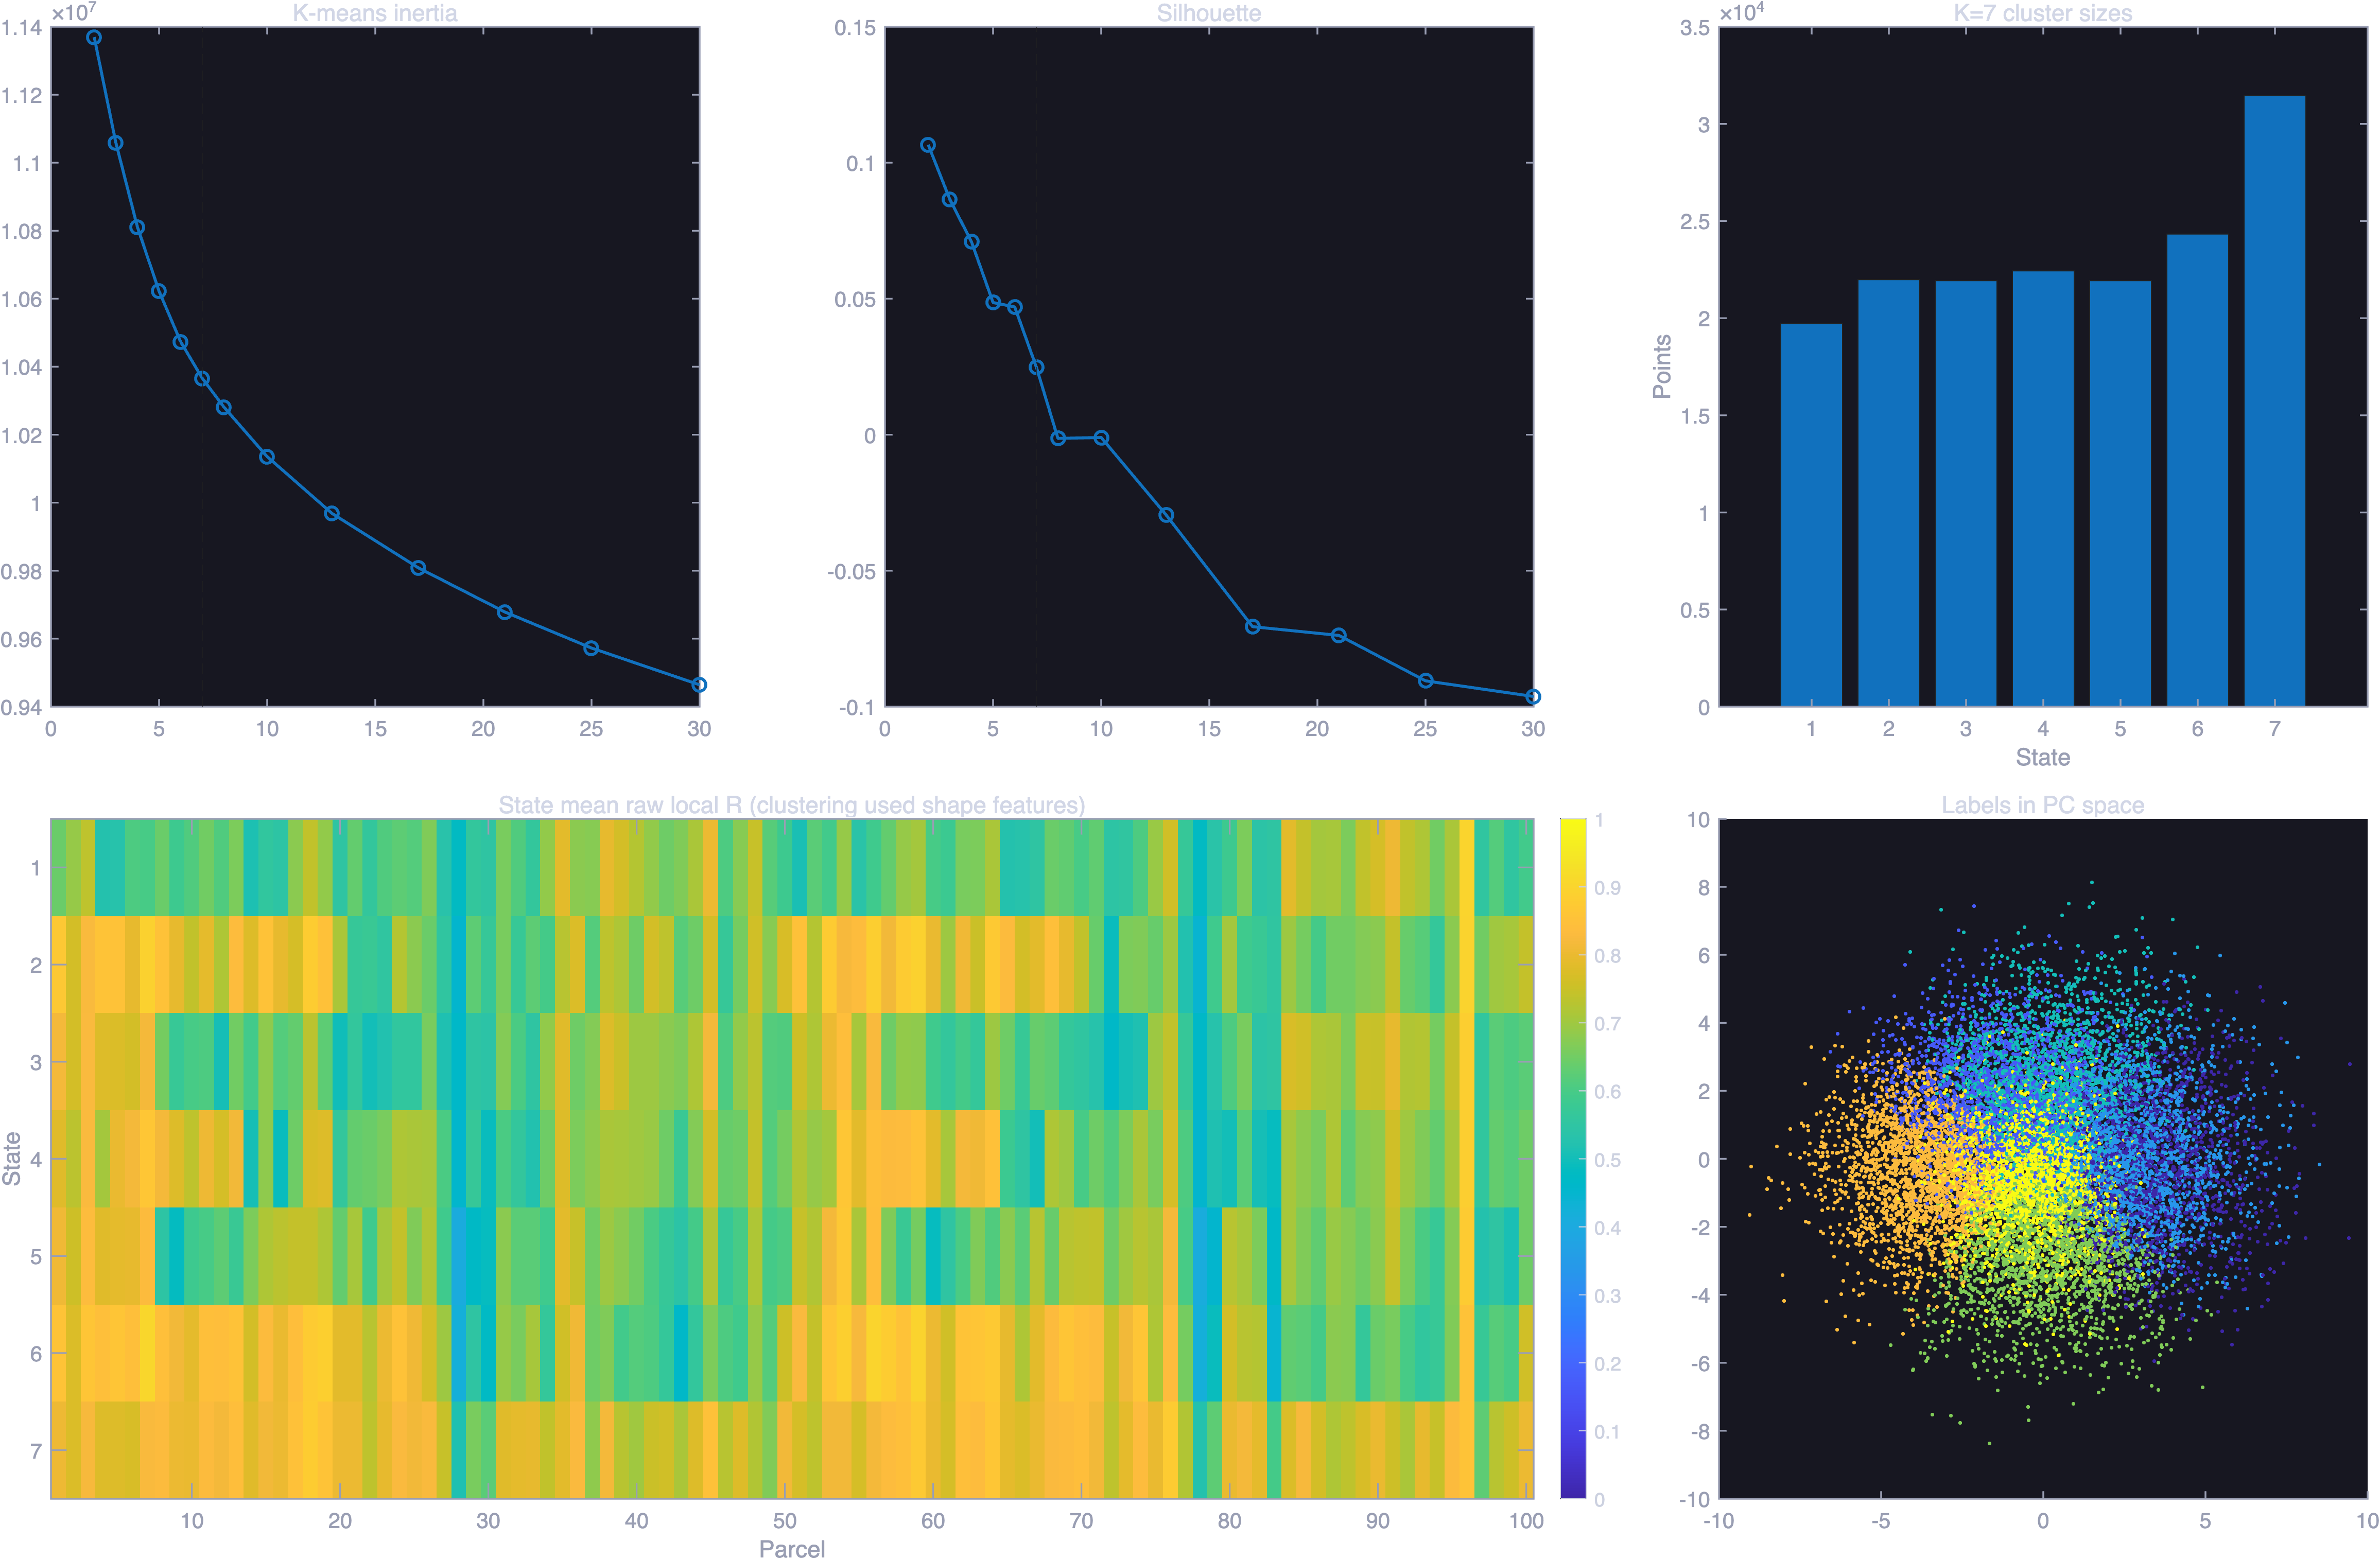
\includegraphics[width=\textwidth]{figures/appendix/a01_state_atlas.png}};
\begin{scope}[x={(image.south east)},y={(image.north west)}]
\node[panel label] at (0.01,0.98) {A};
\node[panel label] at (0.34,0.98) {B};
\node[panel label] at (0.68,0.98) {C};
\node[panel label] at (0.01,0.56) {D};
\node[panel label] at (0.68,0.56) {E};
\end{scope}
\end{tikzpicture}
\caption{\textbf{Seven-state synchronization atlas and clustering diagnostics.}
\textbf{(A)} K-means inertia across candidate state counts.
\textbf{(B)} Mean silhouette width across candidate counts.
\textbf{(C)} Number of volumes assigned to each of the seven states.
\textbf{(D)} State-centroid profiles in local-synchronization space.
\textbf{(E)} State labels projected onto the first two principal components.
The seven-state solution is treated as a predefined working atlas rather than an optimal discrete partition.}
\label{fig:app-state-atlas}
\end{figure}

\begin{figure}[p]
\centering
\begin{tikzpicture}
\node[anchor=south west,inner sep=0] (image) at (0,0)
  {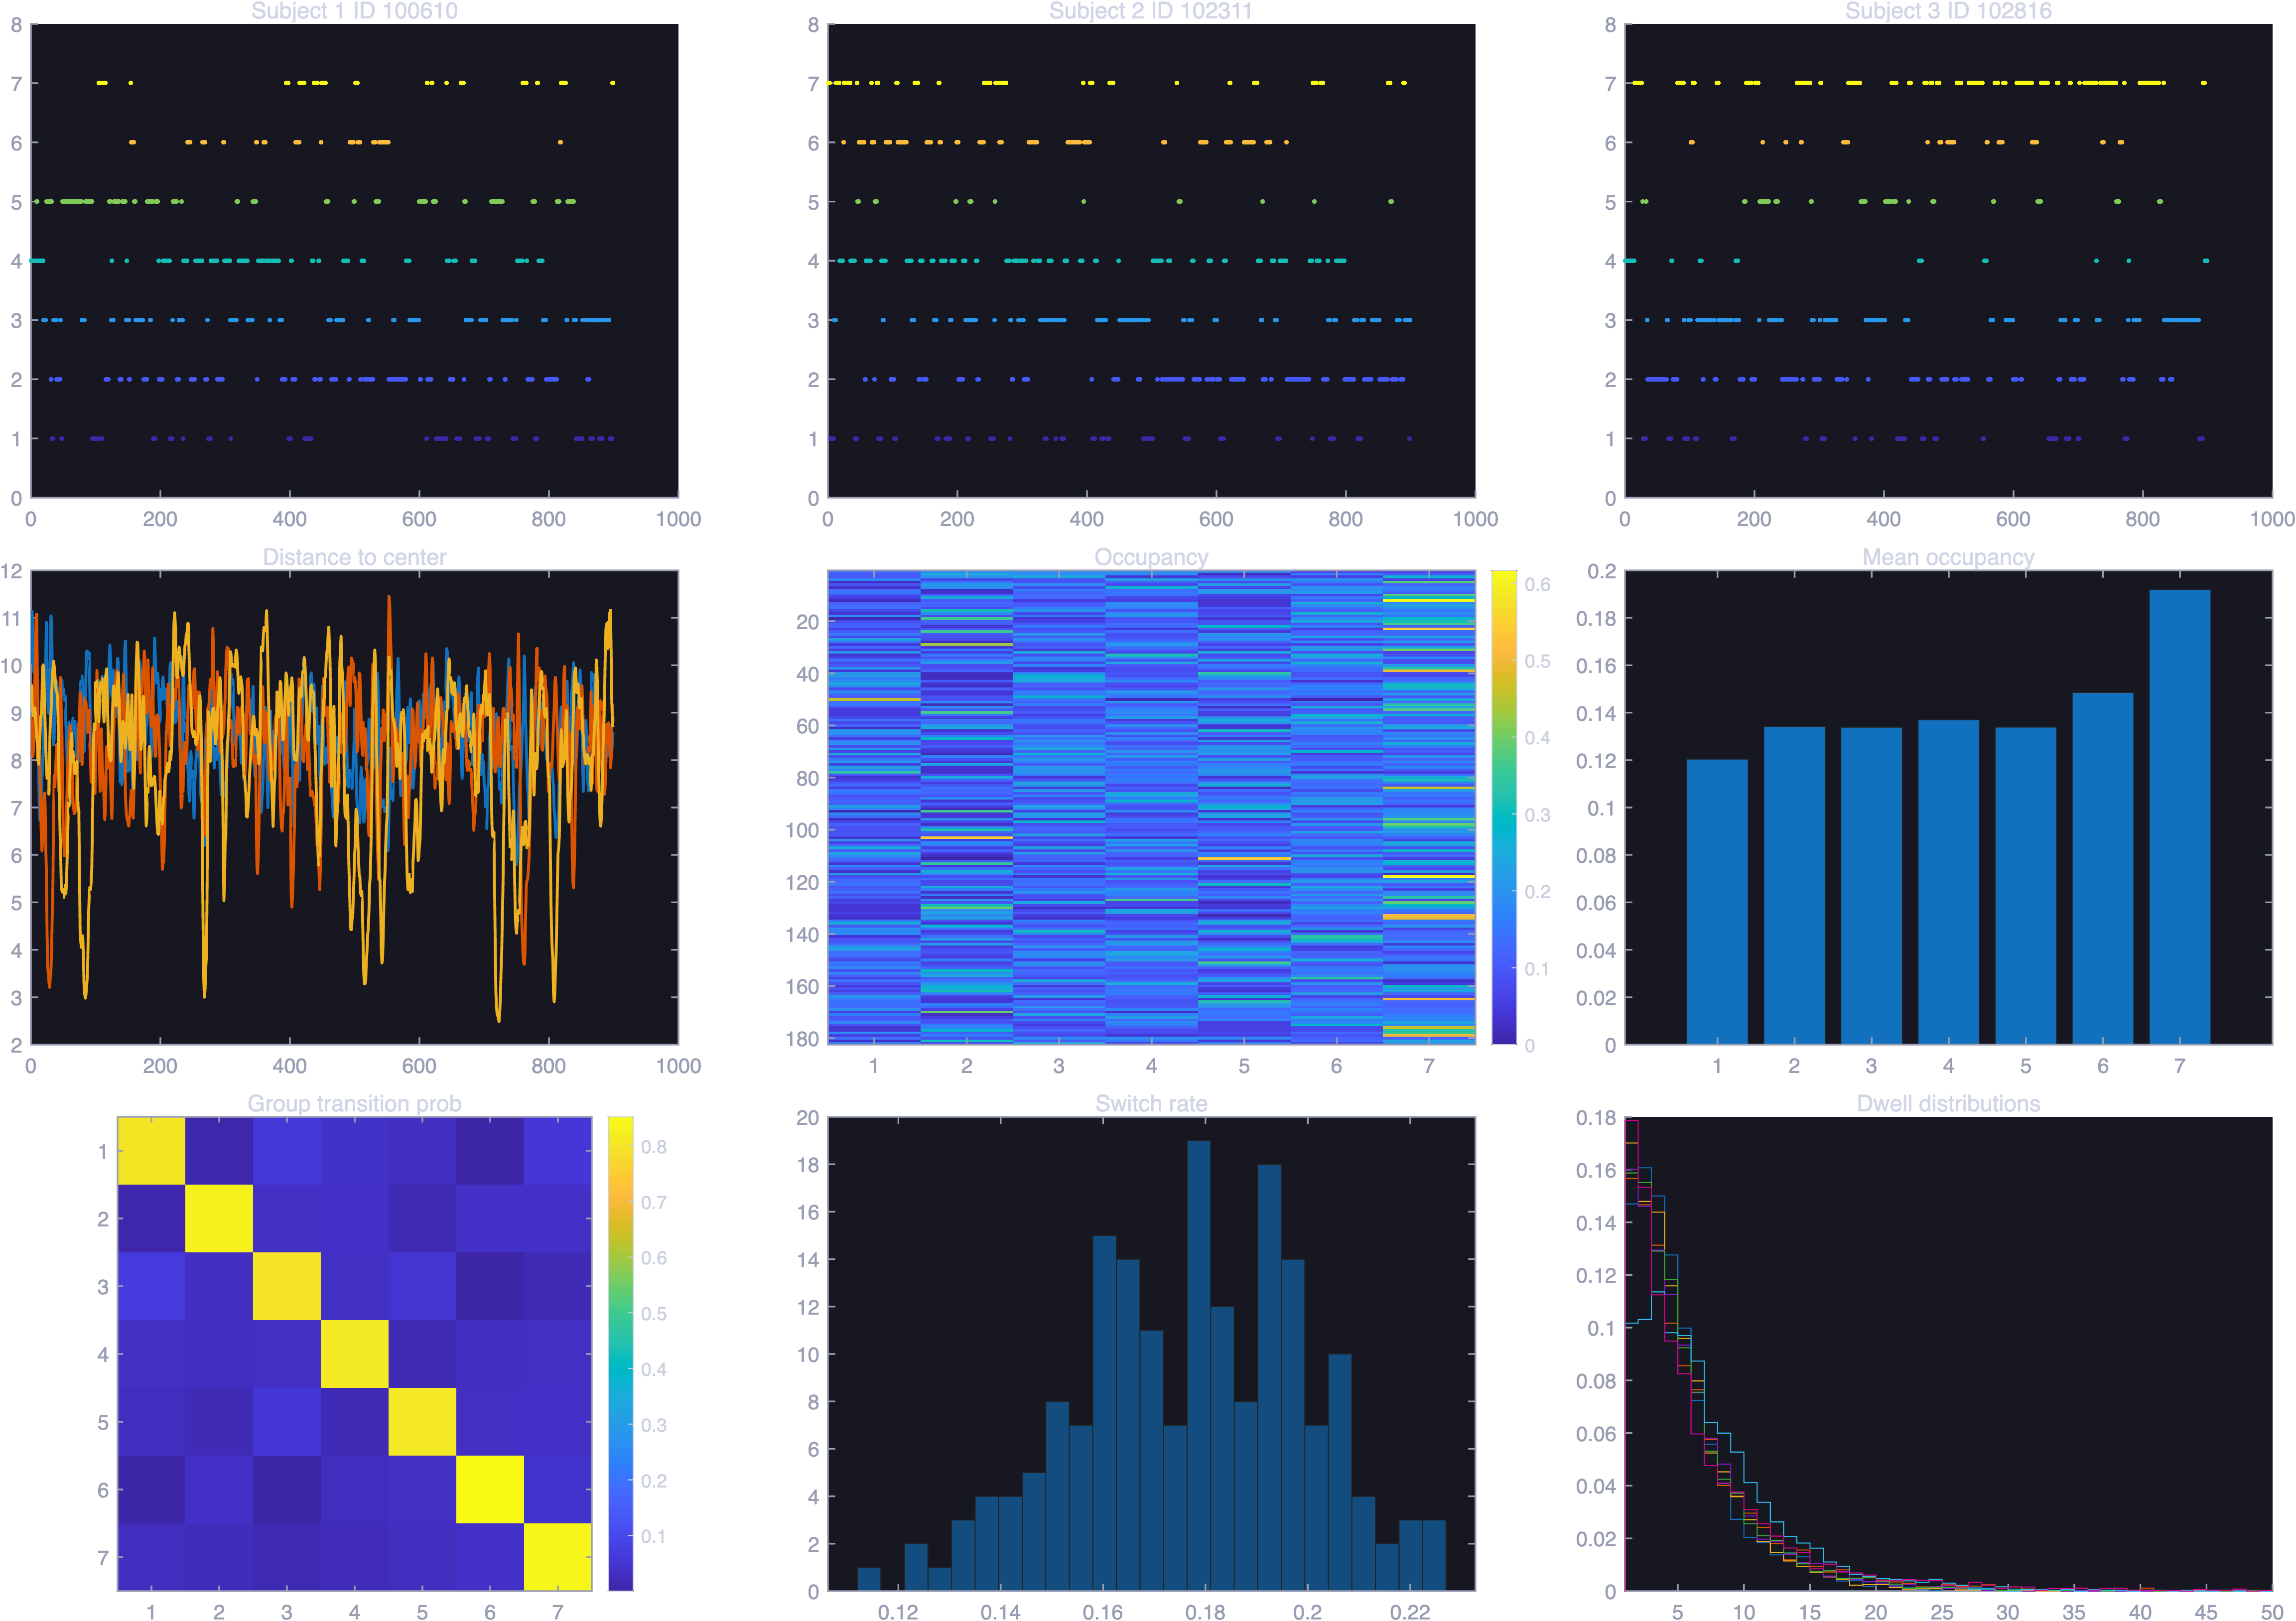
\includegraphics[width=\textwidth]{figures/appendix/a02_state_dynamics.png}};
\begin{scope}[x={(image.south east)},y={(image.north west)}]
\node[panel label] at (0.01,0.98) {A};
\node[panel label] at (0.34,0.98) {B};
\node[panel label] at (0.67,0.98) {C};
\node[panel label] at (0.01,0.65) {D};
\node[panel label] at (0.34,0.65) {E};
\node[panel label] at (0.67,0.65) {F};
\node[panel label] at (0.01,0.32) {G};
\node[panel label] at (0.34,0.32) {H};
\node[panel label] at (0.67,0.32) {I};
\end{scope}
\end{tikzpicture}
\caption{\textbf{State assignments and participant-level dynamic summaries.}
\textbf{(A--C)} Example state sequences for three participants.
\textbf{(D)} Distance of each volume from its assigned centroid.
\textbf{(E)} Participant-by-state occupancy matrix.
\textbf{(F)} Mean occupancy of each state.
\textbf{(G)} Pooled group transition-probability matrix.
\textbf{(H)} Distribution of participant switch rates.
\textbf{(I)} State-specific dwell-time distributions.}
\label{fig:app-state-dynamics}
\end{figure}

\begin{figure}[p]
\centering
\begin{tikzpicture}
\node[anchor=south west,inner sep=0] (image) at (0,0)
  {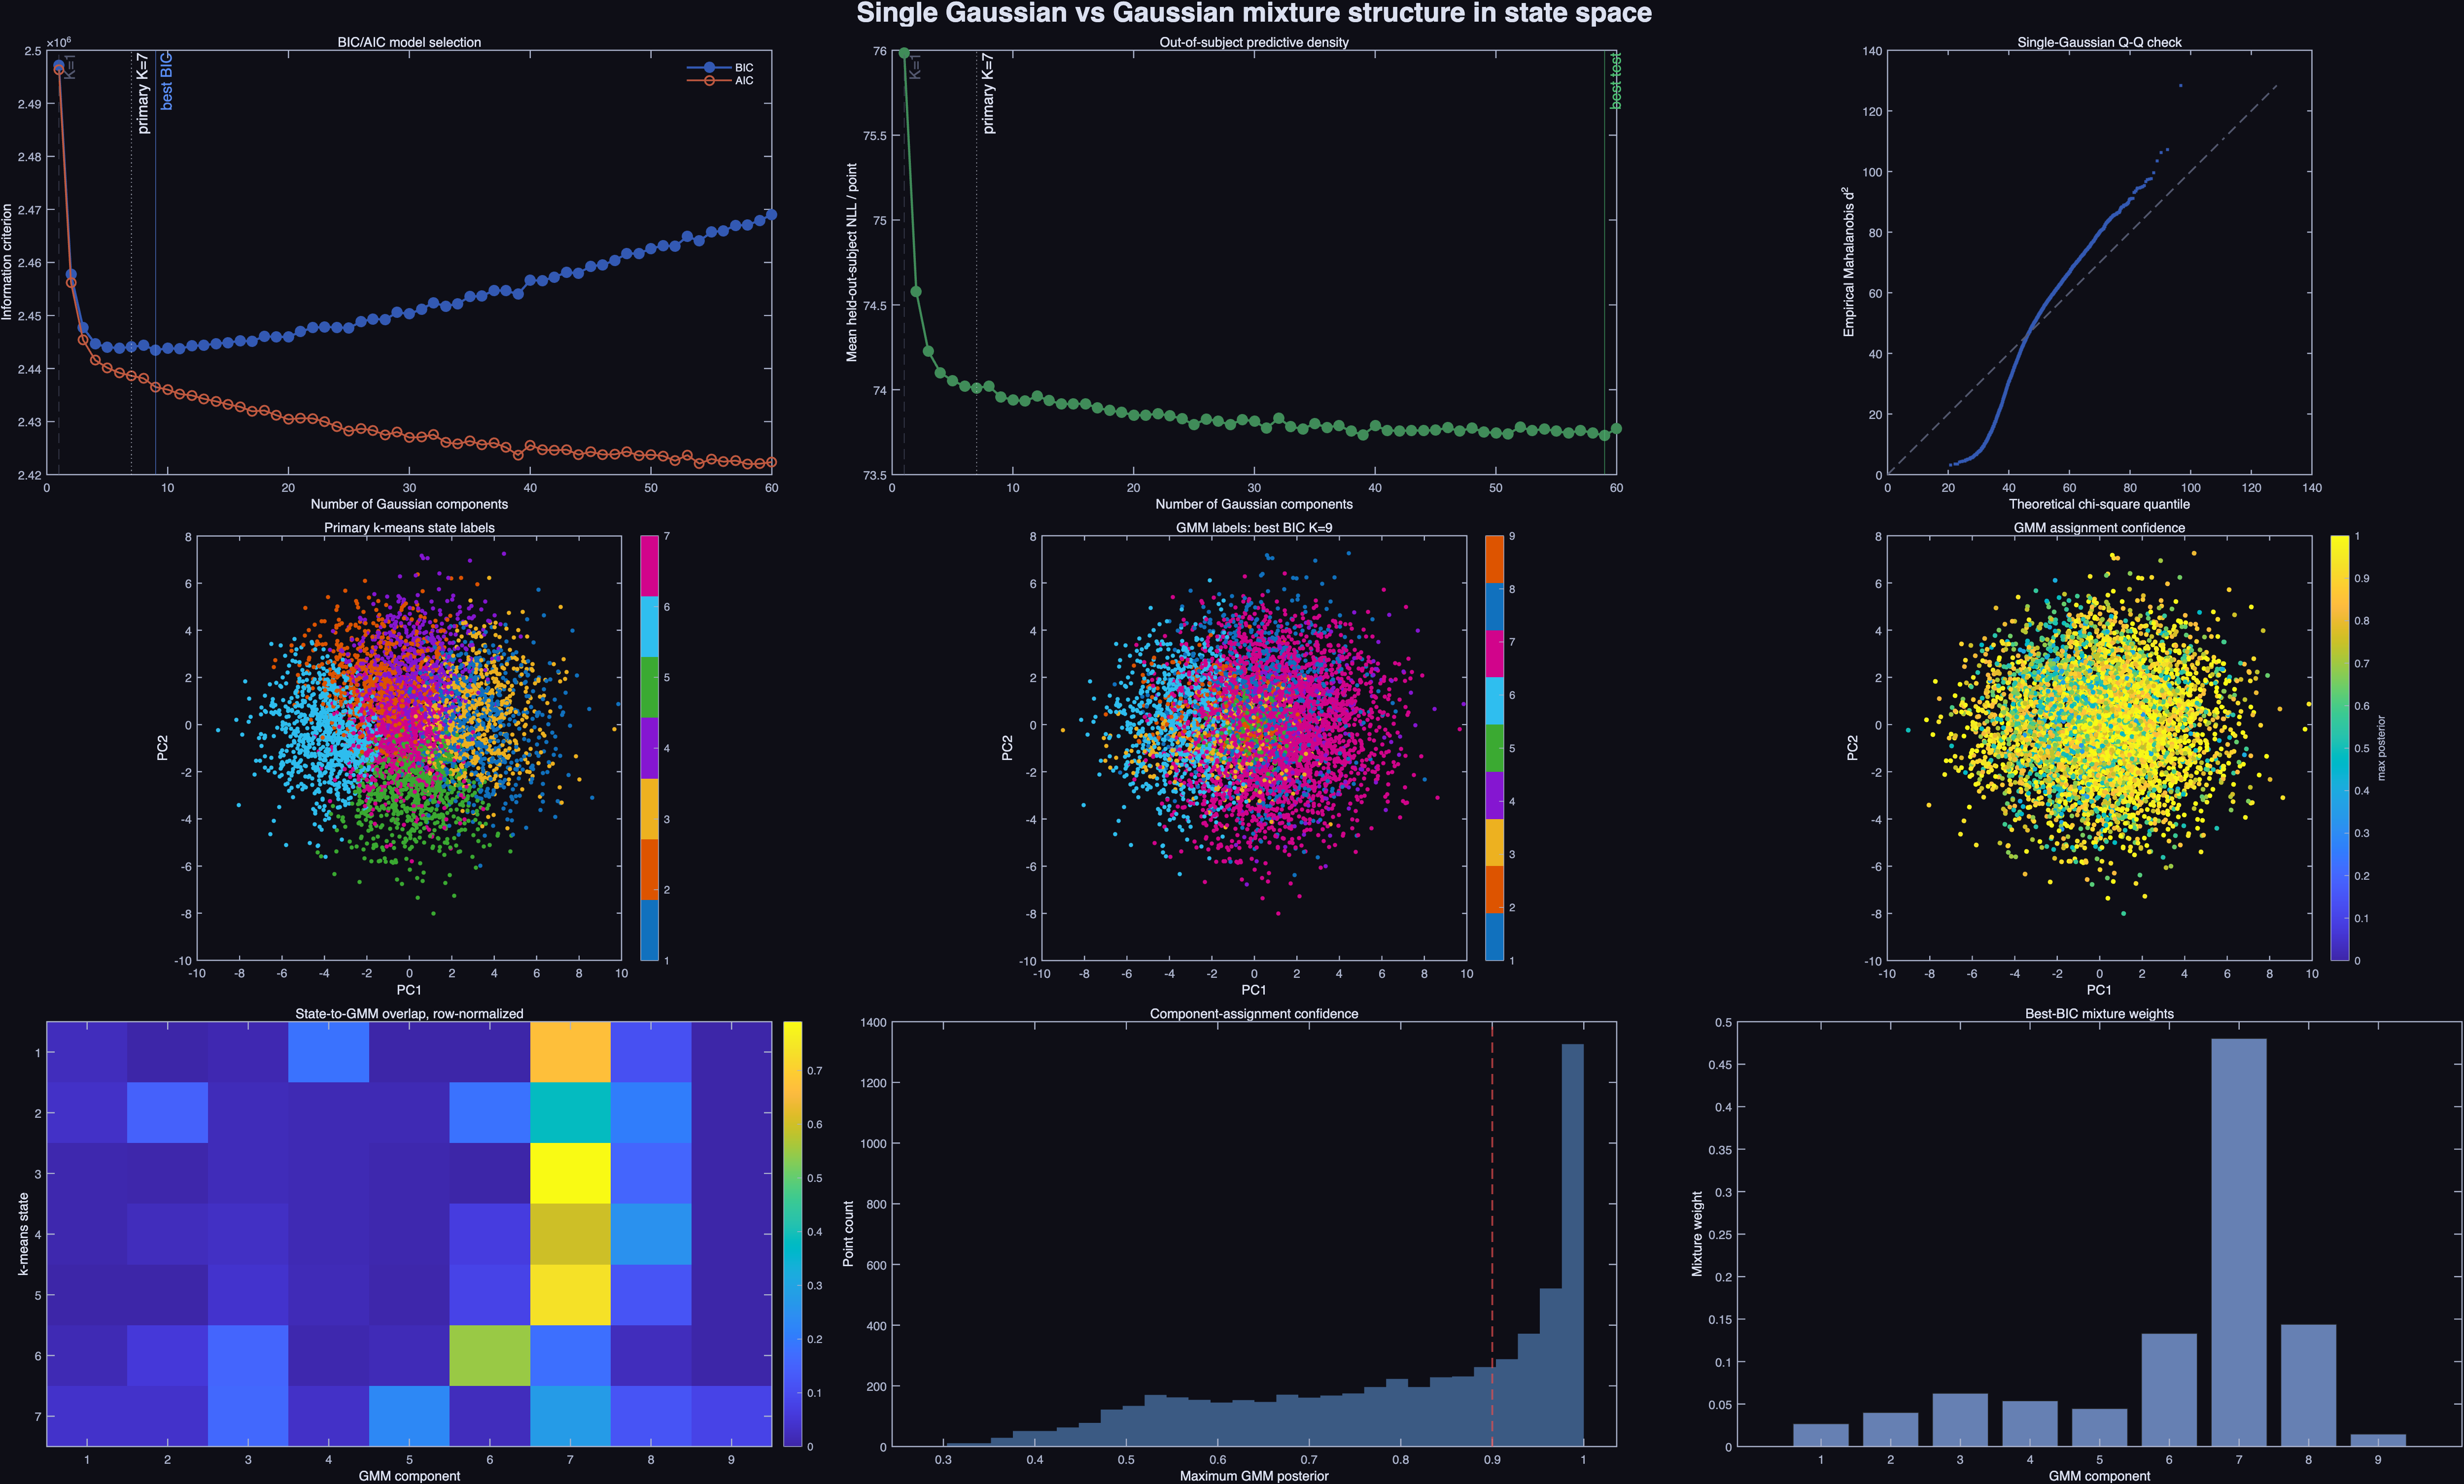
\includegraphics[width=\textwidth]{figures/appendix/a03_gmm_validation.png}};
\begin{scope}[x={(image.south east)},y={(image.north west)}]
\node[panel label] at (0.01,0.98) {A};
\node[panel label] at (0.34,0.98) {B};
\node[panel label] at (0.67,0.98) {C};
\node[panel label] at (0.01,0.65) {D};
\node[panel label] at (0.34,0.65) {E};
\node[panel label] at (0.67,0.65) {F};
\node[panel label] at (0.01,0.32) {G};
\node[panel label] at (0.34,0.32) {H};
\node[panel label] at (0.67,0.32) {I};
\end{scope}
\end{tikzpicture}
\caption{\textbf{Gaussian-mixture validation of the synchronization state space.}
\textbf{(A)} BIC and AIC across candidate mixture sizes.
\textbf{(B)} Participant-blocked out-of-sample predictive density.
\textbf{(C)} Quantile diagnostic for a single Gaussian.
\textbf{(D)} K-means labels in the first two principal components.
\textbf{(E)} Best-BIC mixture assignments in the same projection.
\textbf{(F)} Posterior assignment confidence.
\textbf{(G)} Overlap between atlas states and mixture components.
\textbf{(H)} Distribution of assignment confidence.
\textbf{(I)} Best-BIC mixture weights.}
\label{fig:app-gmm-validation}
\end{figure}

\begin{figure}[p]
\centering
\begin{tikzpicture}
\node[anchor=south west,inner sep=0] (image) at (0,0)
  {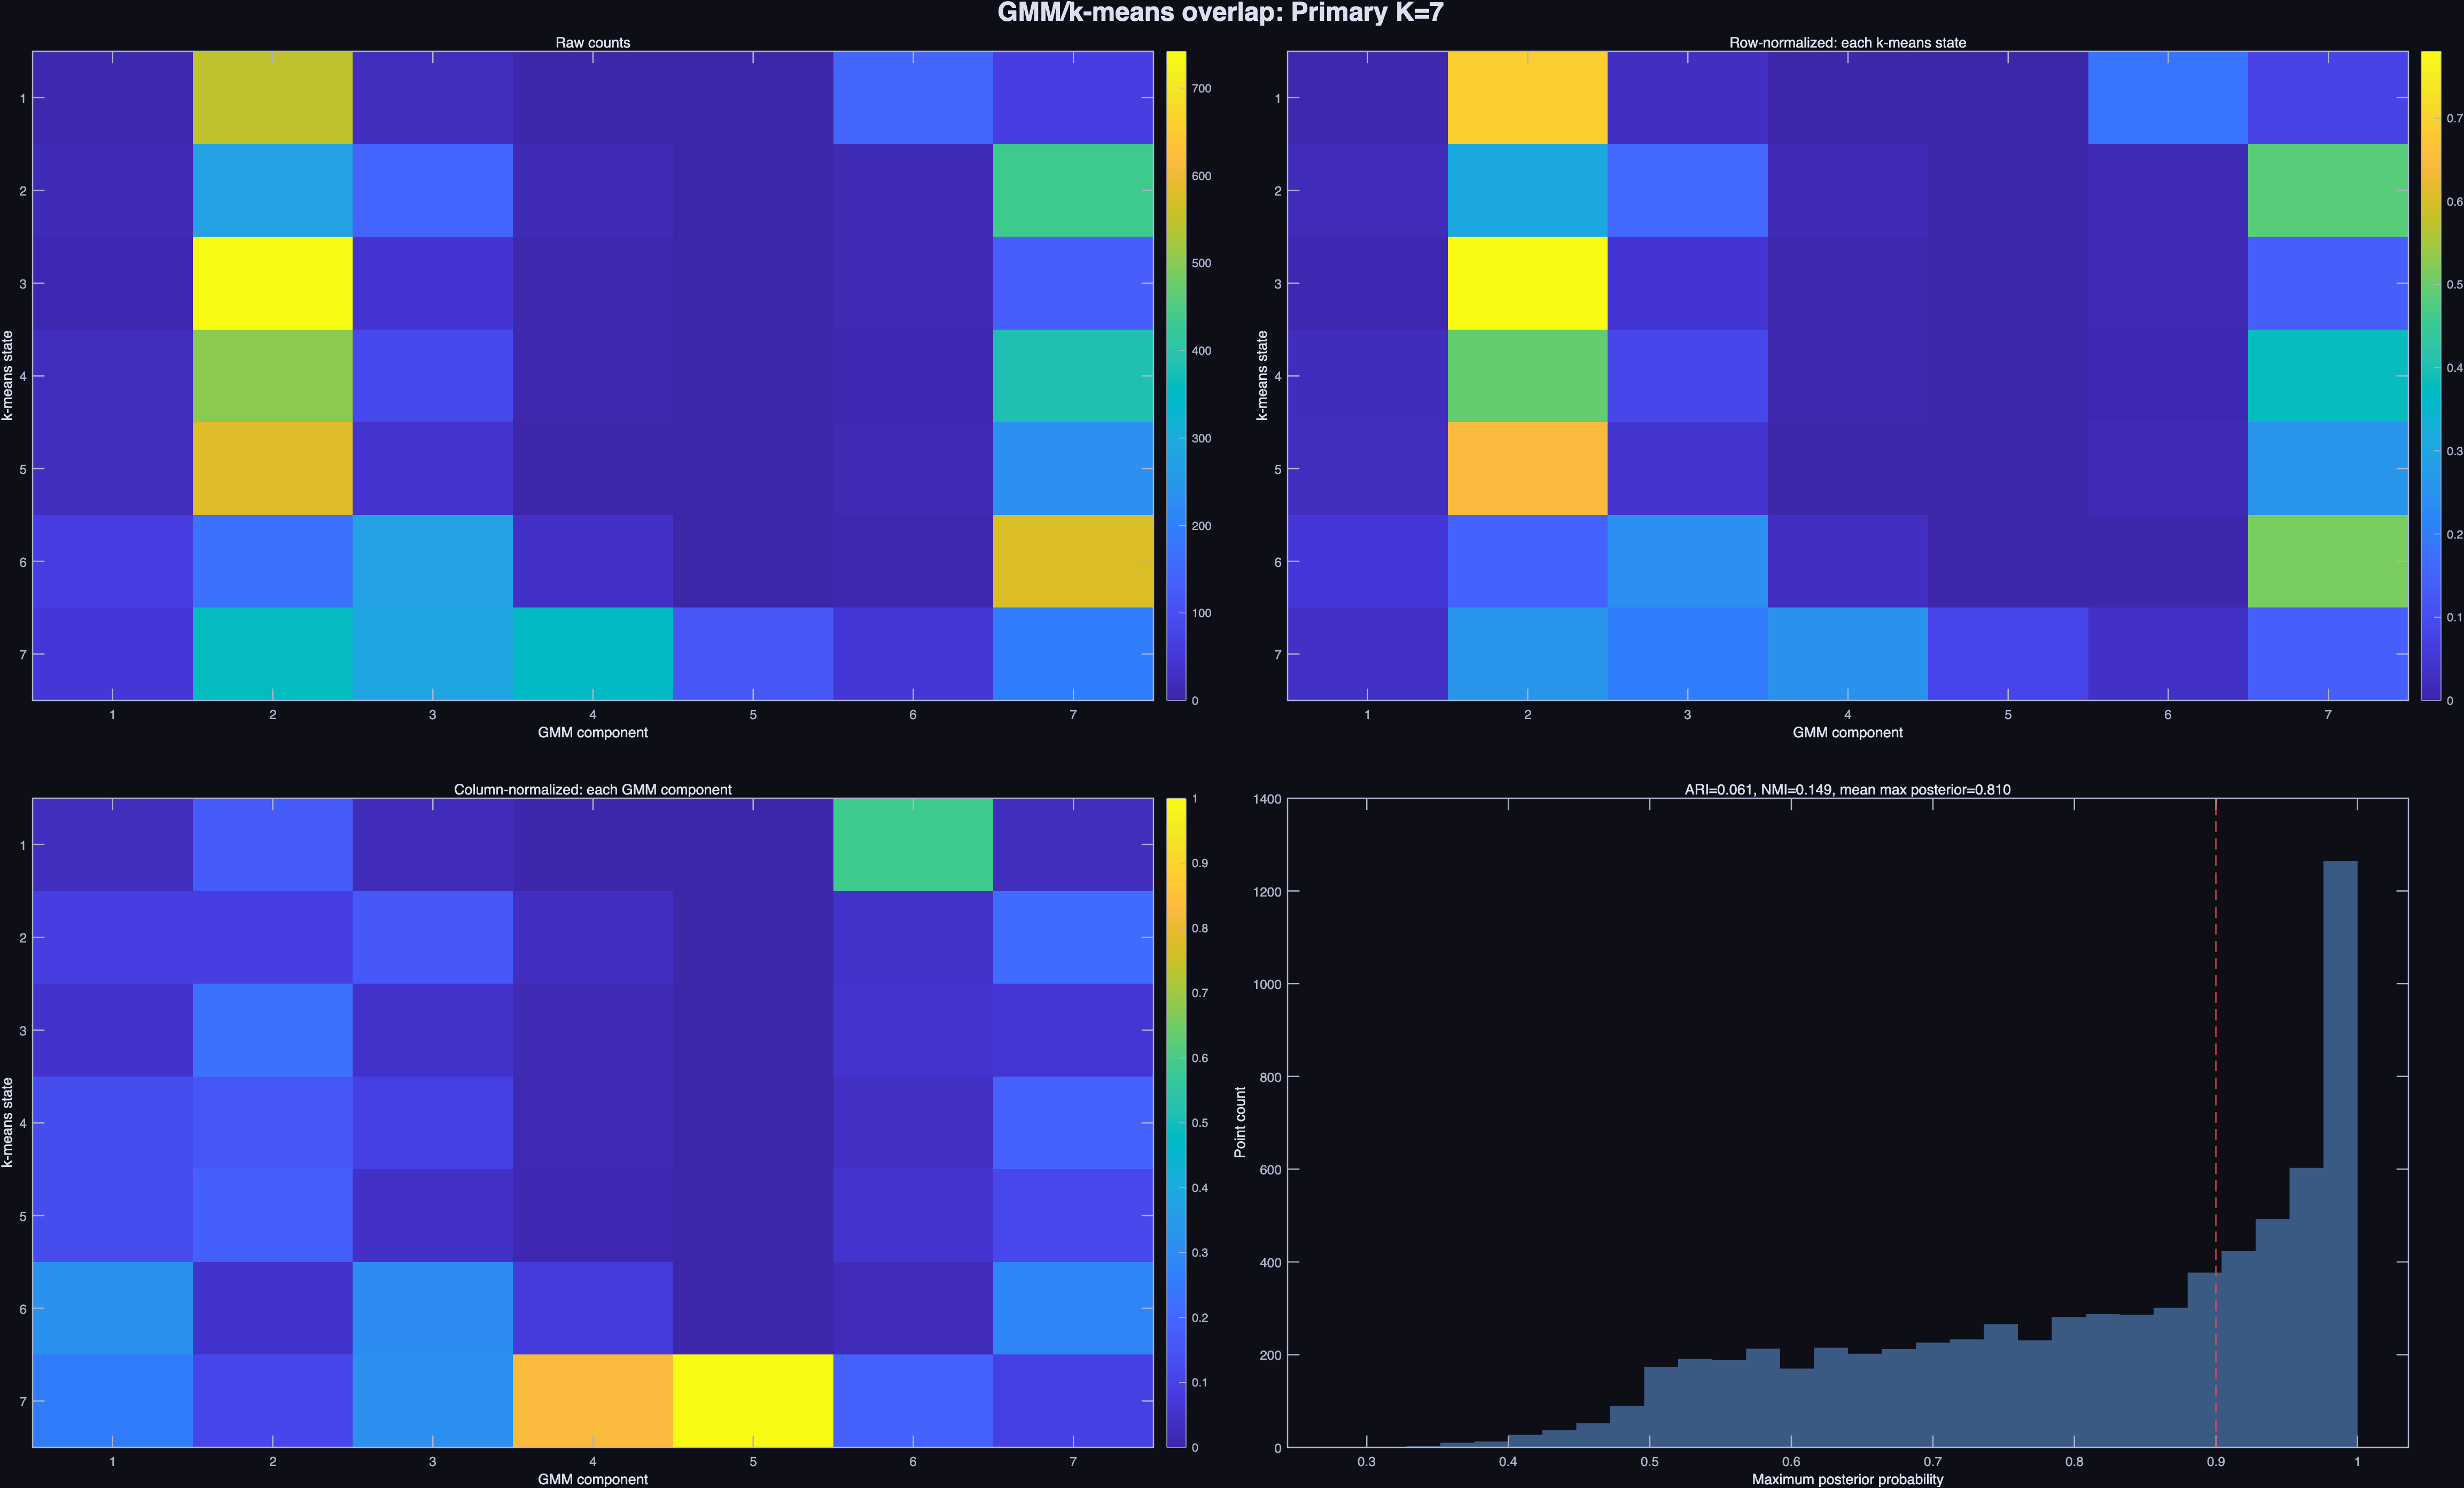
\includegraphics[width=\textwidth]{figures/appendix/a04_gmm_overlap_k7.png}};
\begin{scope}[x={(image.south east)},y={(image.north west)}]
\node[panel label] at (0.01,0.98) {A};
\node[panel label] at (0.51,0.98) {B};
\node[panel label] at (0.01,0.49) {C};
\node[panel label] at (0.51,0.49) {D};
\end{scope}
\end{tikzpicture}
\caption{\textbf{Overlap between the seven-state atlas and a seven-component Gaussian mixture.}
\textbf{(A)} Raw state-by-component counts.
\textbf{(B)} Row-normalized overlap.
\textbf{(C)} Column-normalized overlap.
\textbf{(D)} Posterior assignment-confidence distribution.
The low adjusted Rand index indicates that the mixture does not recover the predefined atlas partition.}
\label{fig:app-gmm-overlap}
\end{figure}

\clearpage
\section{Transition structure and generative models}

\begin{figure}[htbp]
\centering
\begin{tikzpicture}
\node[anchor=south west,inner sep=0] (image) at (0,0)
  {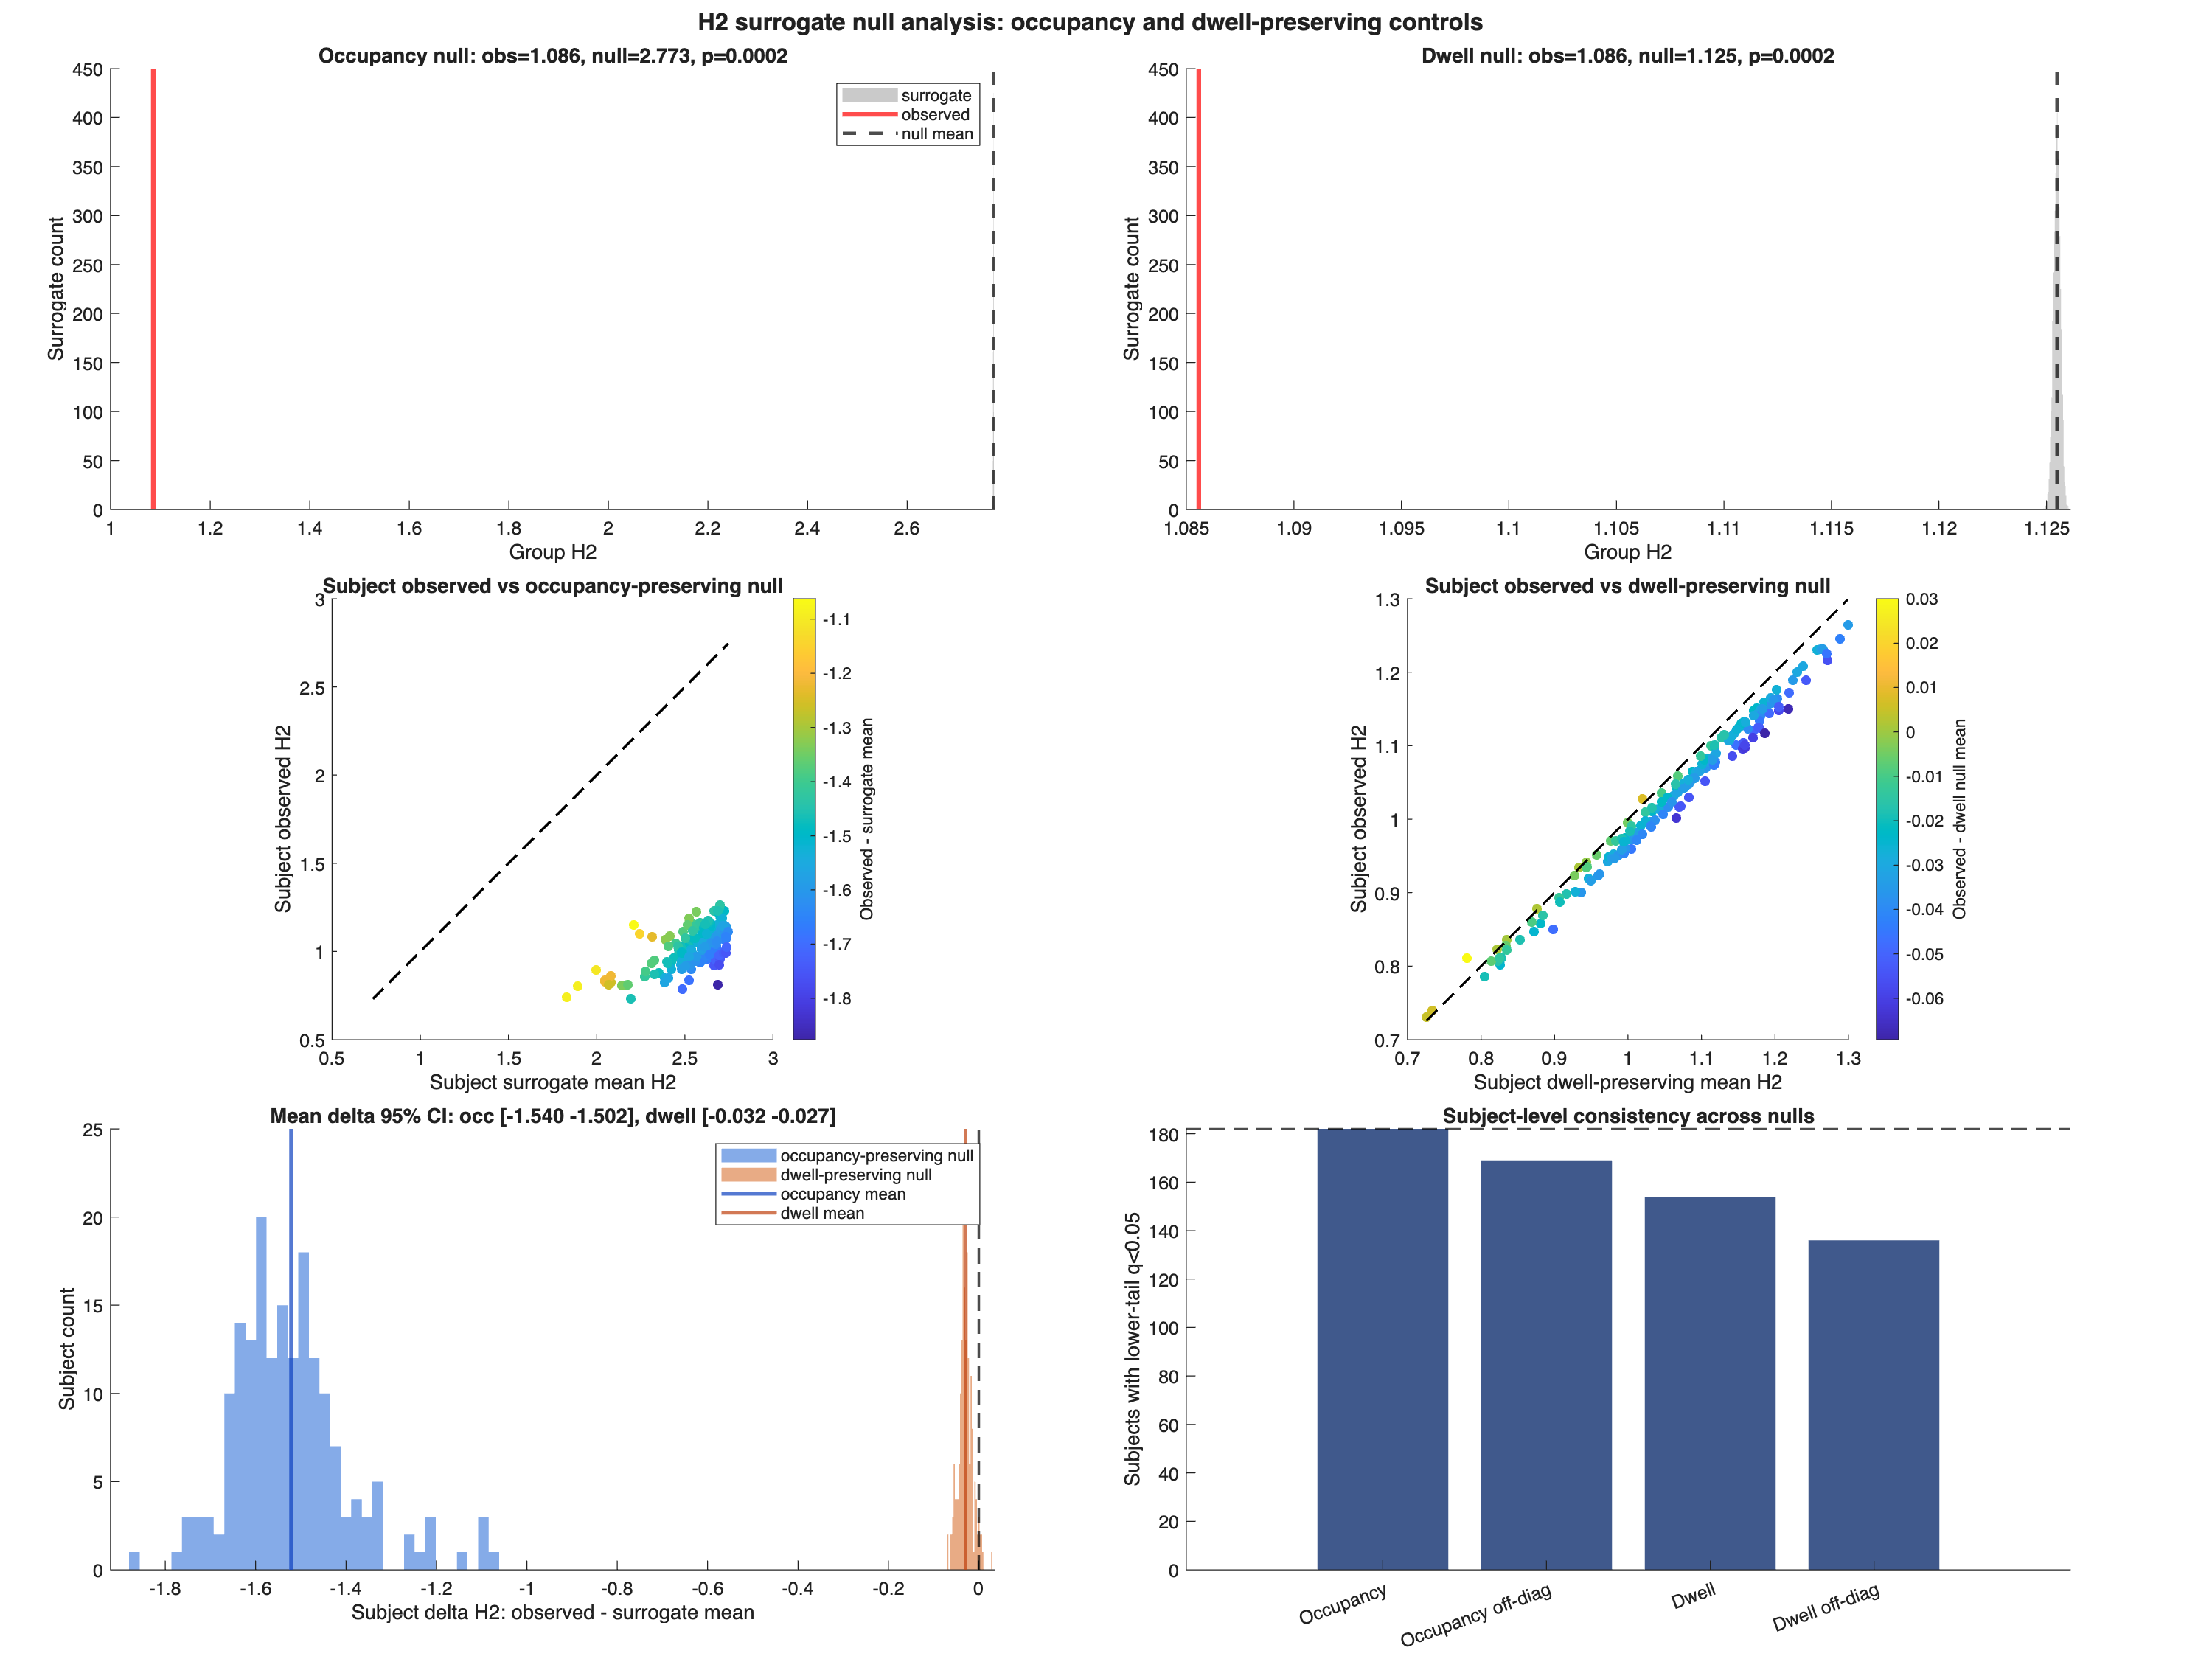
\includegraphics[width=\textwidth]{figures/appendix/a05_surrogate_nulls.png}};
\begin{scope}[x={(image.south east)},y={(image.north west)}]
\node[panel label] at (0.01,0.98) {A};
\node[panel label] at (0.51,0.98) {B};
\node[panel label] at (0.01,0.65) {C};
\node[panel label] at (0.51,0.65) {D};
\node[panel label] at (0.01,0.32) {E};
\node[panel label] at (0.51,0.32) {F};
\end{scope}
\end{tikzpicture}
\caption{\textbf{Occupancy- and dwell-preserving surrogate-null analyses.}
\textbf{(A)} Pooled observed entropy against the occupancy-preserving null.
\textbf{(B)} Pooled observed entropy against the dwell-preserving null.
\textbf{(C)} Participant observed-versus-null values for the occupancy null.
\textbf{(D)} Participant observed-versus-null values for the dwell null.
\textbf{(E)} Participant observed-minus-null differences.
\textbf{(F)} Number of participants with corrected lower-tail results.}
\label{fig:app-surrogate-nulls}
\end{figure}

\begin{figure}[p]
\centering
\begin{tikzpicture}
\node[anchor=south west,inner sep=0] (image) at (0,0)
  {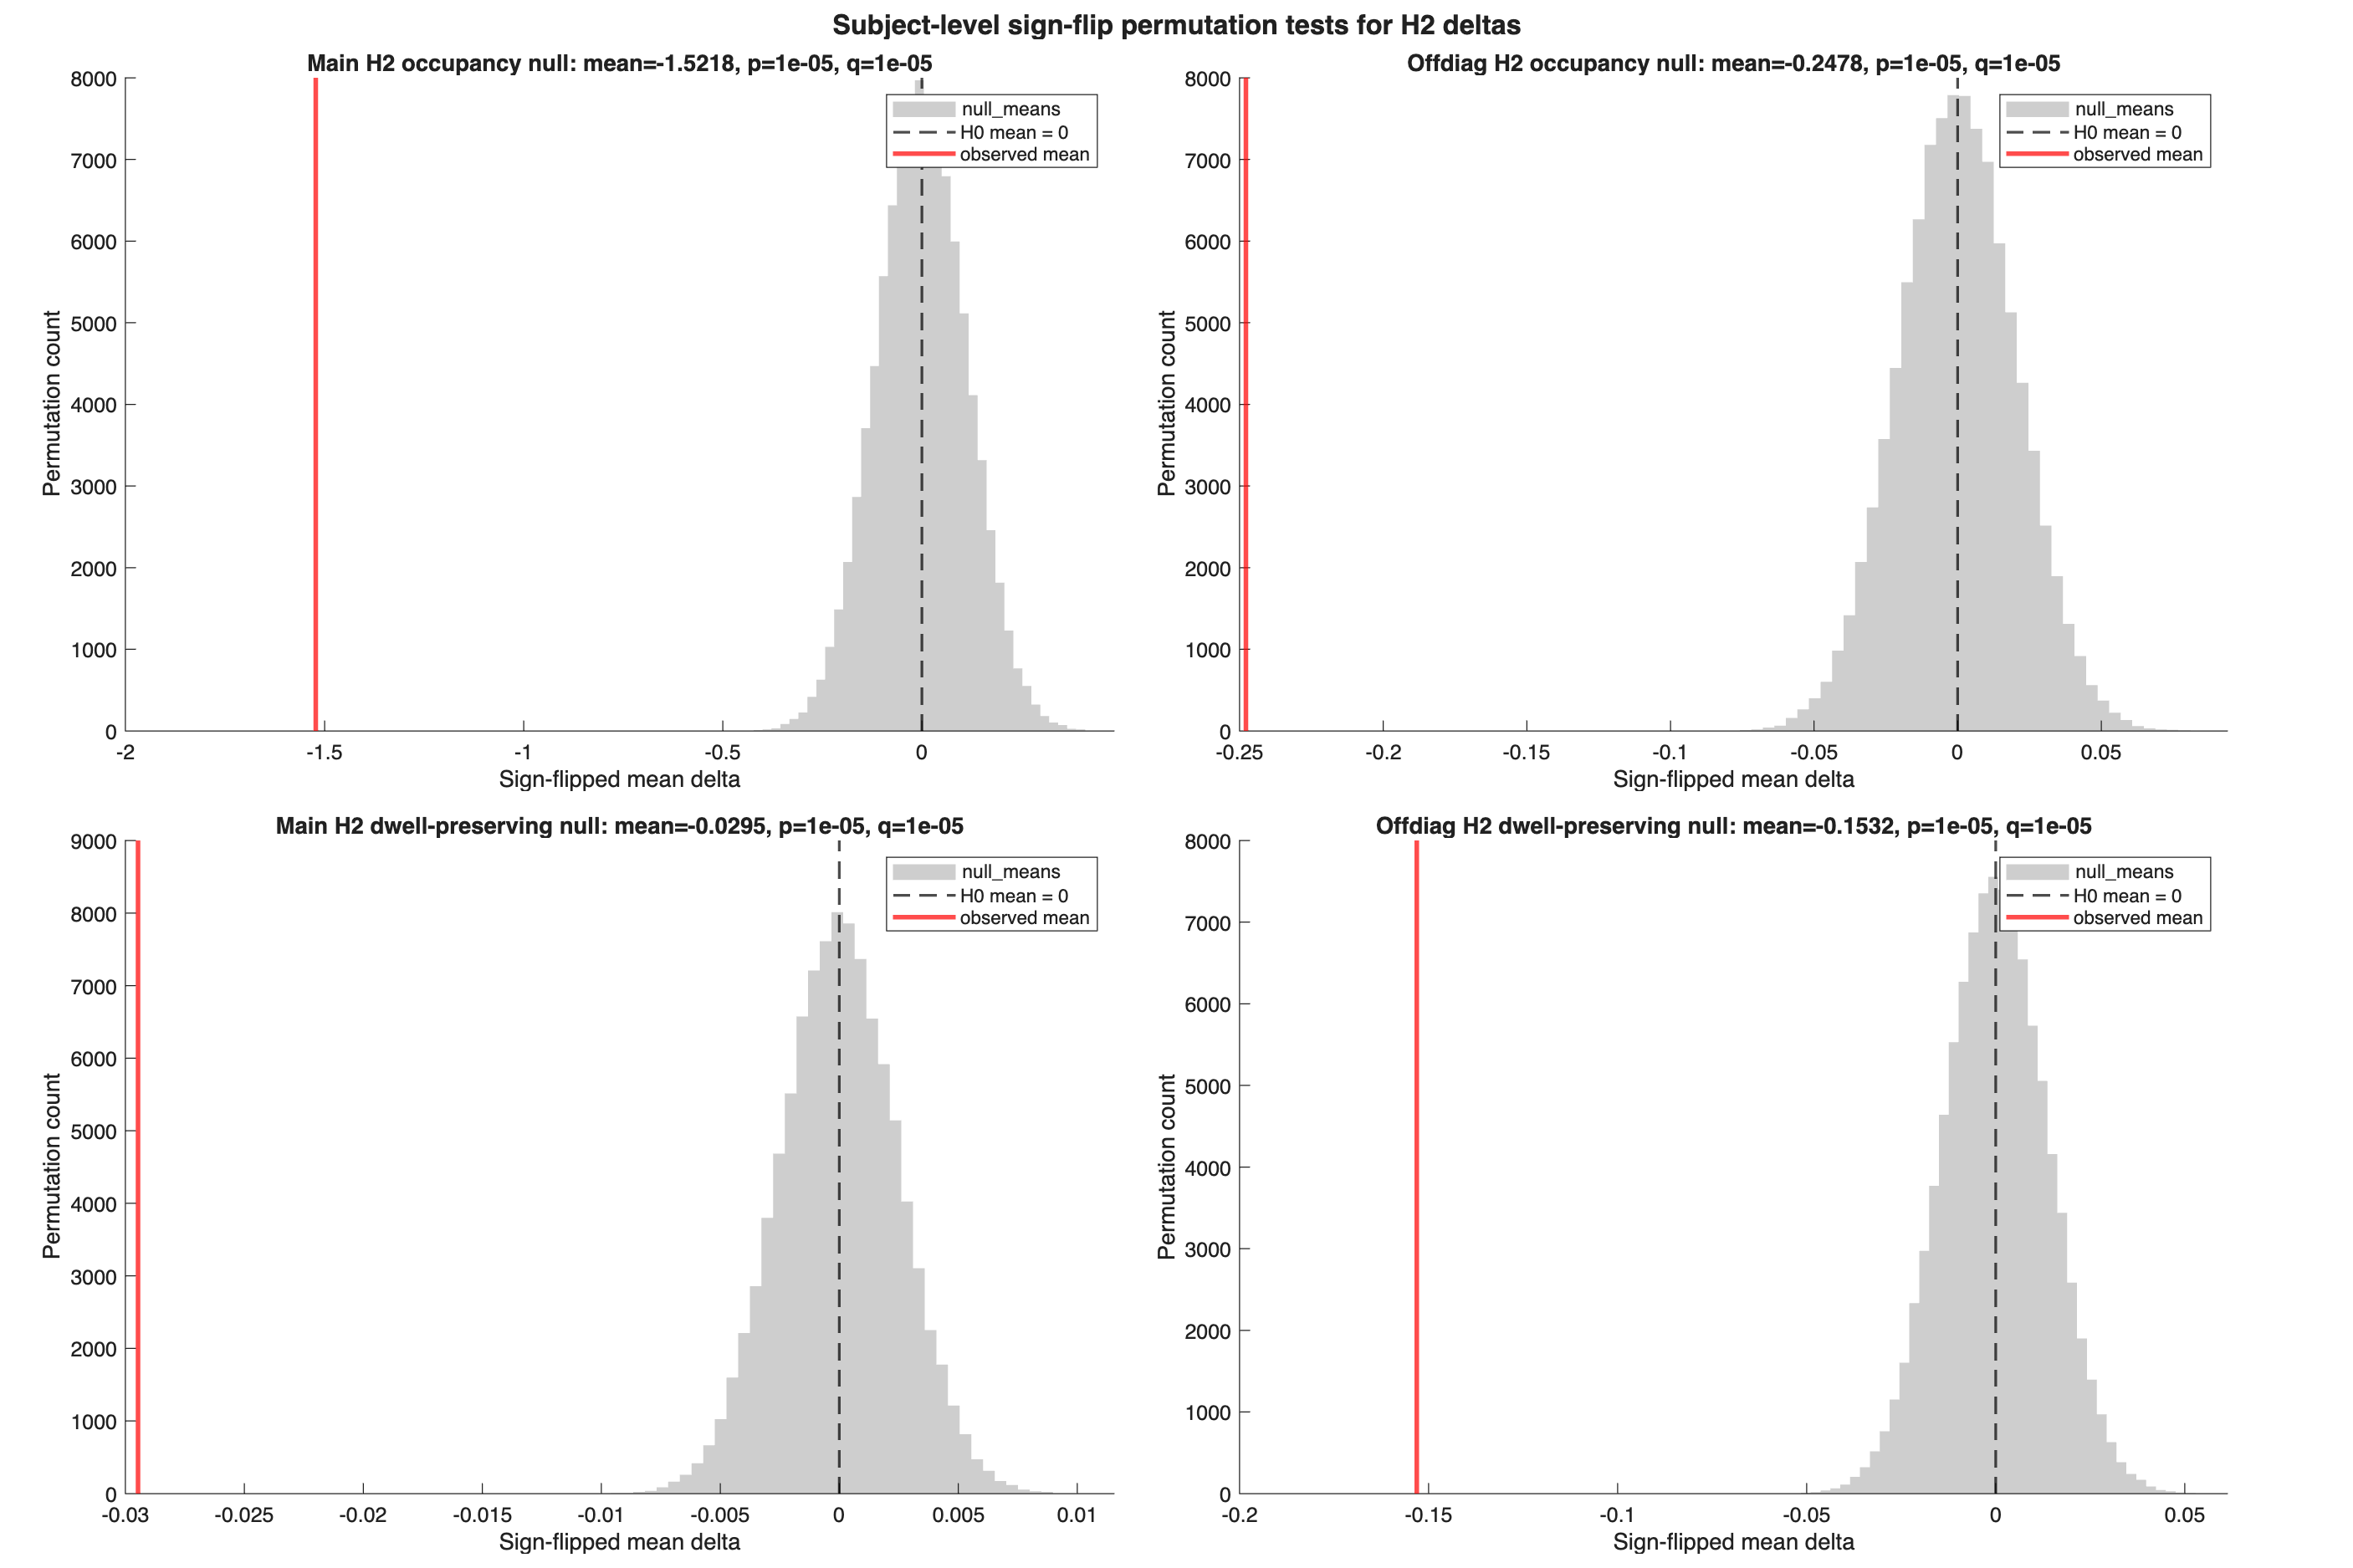
\includegraphics[width=\textwidth]{figures/appendix/a06_surrogate_signflip.png}};
\begin{scope}[x={(image.south east)},y={(image.north west)}]
\node[panel label] at (0.01,0.98) {A};
\node[panel label] at (0.51,0.98) {B};
\node[panel label] at (0.01,0.49) {C};
\node[panel label] at (0.51,0.49) {D};
\end{scope}
\end{tikzpicture}
\caption{\textbf{Participant-level sign-flip tests of transition-entropy differences.}
\textbf{(A)} Full transition entropy under the occupancy-preserving null.
\textbf{(B)} Off-diagonal entropy under the occupancy-preserving null.
\textbf{(C)} Full transition entropy under the dwell-preserving null.
\textbf{(D)} Off-diagonal entropy under the dwell-preserving null.
Red lines mark observed mean differences; negative values indicate lower observed entropy.}
\label{fig:app-surrogate-signflip}
\end{figure}

\begin{figure}[p]
\centering
\begin{tikzpicture}
\node[anchor=south west,inner sep=0] (image) at (0,0)
  {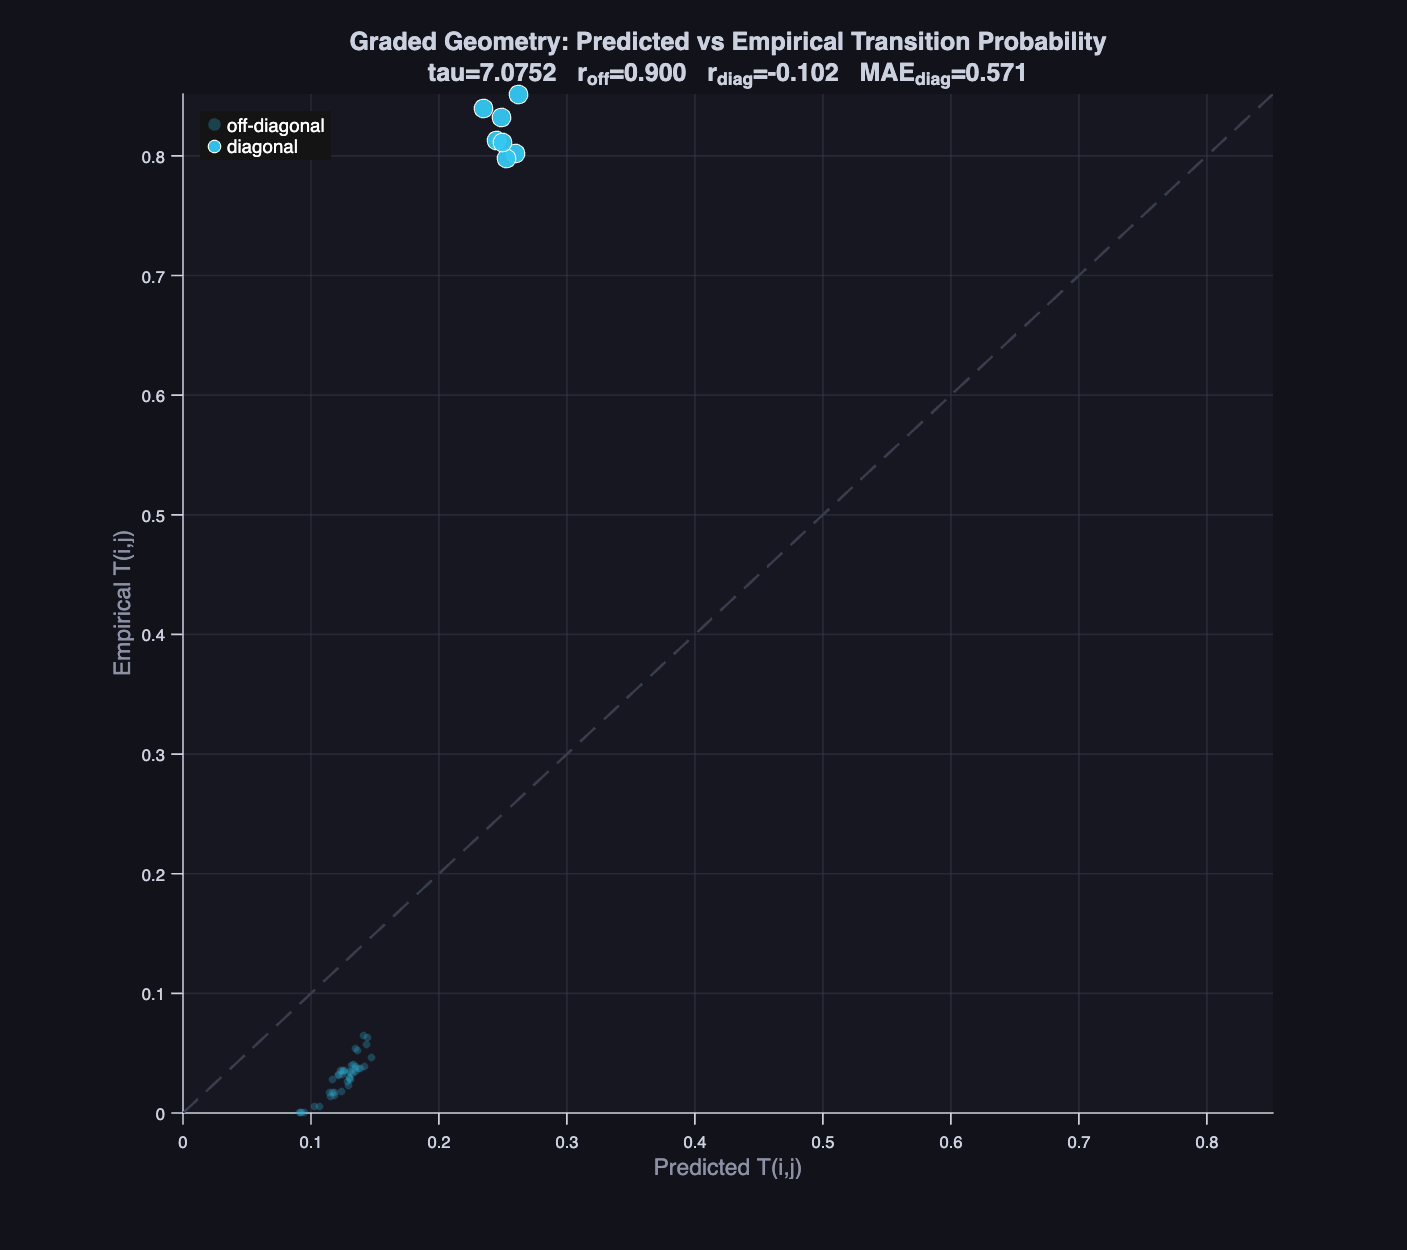
\includegraphics[width=\textwidth]{figures/appendix/a07_geometry_group_fit.png}};
\begin{scope}[x={(image.south east)},y={(image.north west)}]
\node[panel label] at (0.01,0.98) {A};
\end{scope}
\end{tikzpicture}
\caption{\textbf{Full-sample graded-geometry fit.}
\textbf{(A)} Model-predicted versus empirical transition probabilities, distinguishing diagonal persistence from off-diagonal switching. The exponential distance law captures off-diagonal ordering but not the self-transition pattern.}
\label{fig:app-geometry-group}
\end{figure}

\begin{figure}[p]
\centering
\begin{tikzpicture}
\node[anchor=south west,inner sep=0] (image) at (0,0)
  {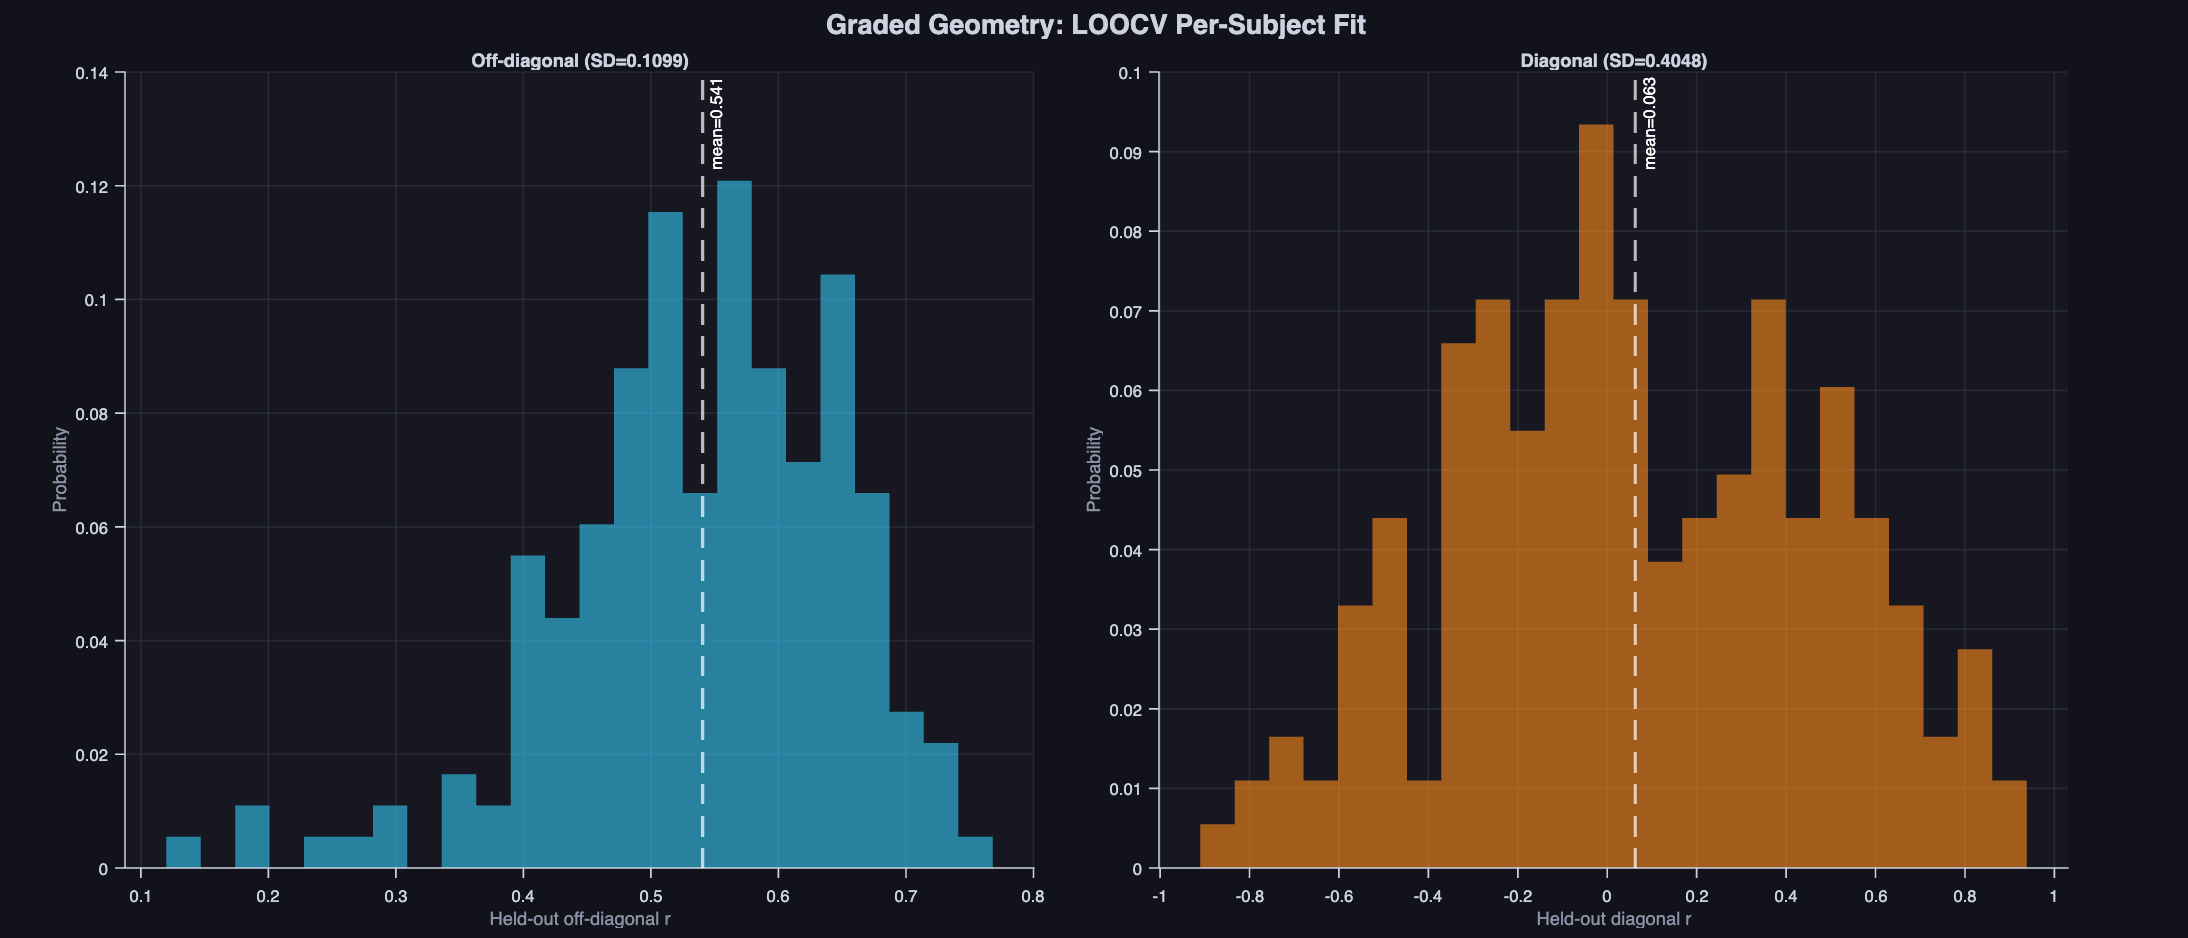
\includegraphics[width=\textwidth]{figures/appendix/a08_geometry_loocv.png}};
\begin{scope}[x={(image.south east)},y={(image.north west)}]
\node[panel label] at (0.01,0.98) {A};
\node[panel label] at (0.51,0.98) {B};
\end{scope}
\end{tikzpicture}
\caption{\textbf{Held-out graded-geometry fit across participants.}
\textbf{(A)} Leave-one-participant-out correlations for off-diagonal switch routing.
\textbf{(B)} Corresponding correlations for diagonal persistence.
Off-diagonal correlations are consistently positive, whereas diagonal correlations are broad and centred near zero.}
\label{fig:app-geometry-loocv}
\end{figure}

\begin{figure}[p]
\centering
\begin{tikzpicture}
\node[anchor=south west,inner sep=0] (image) at (0,0)
  {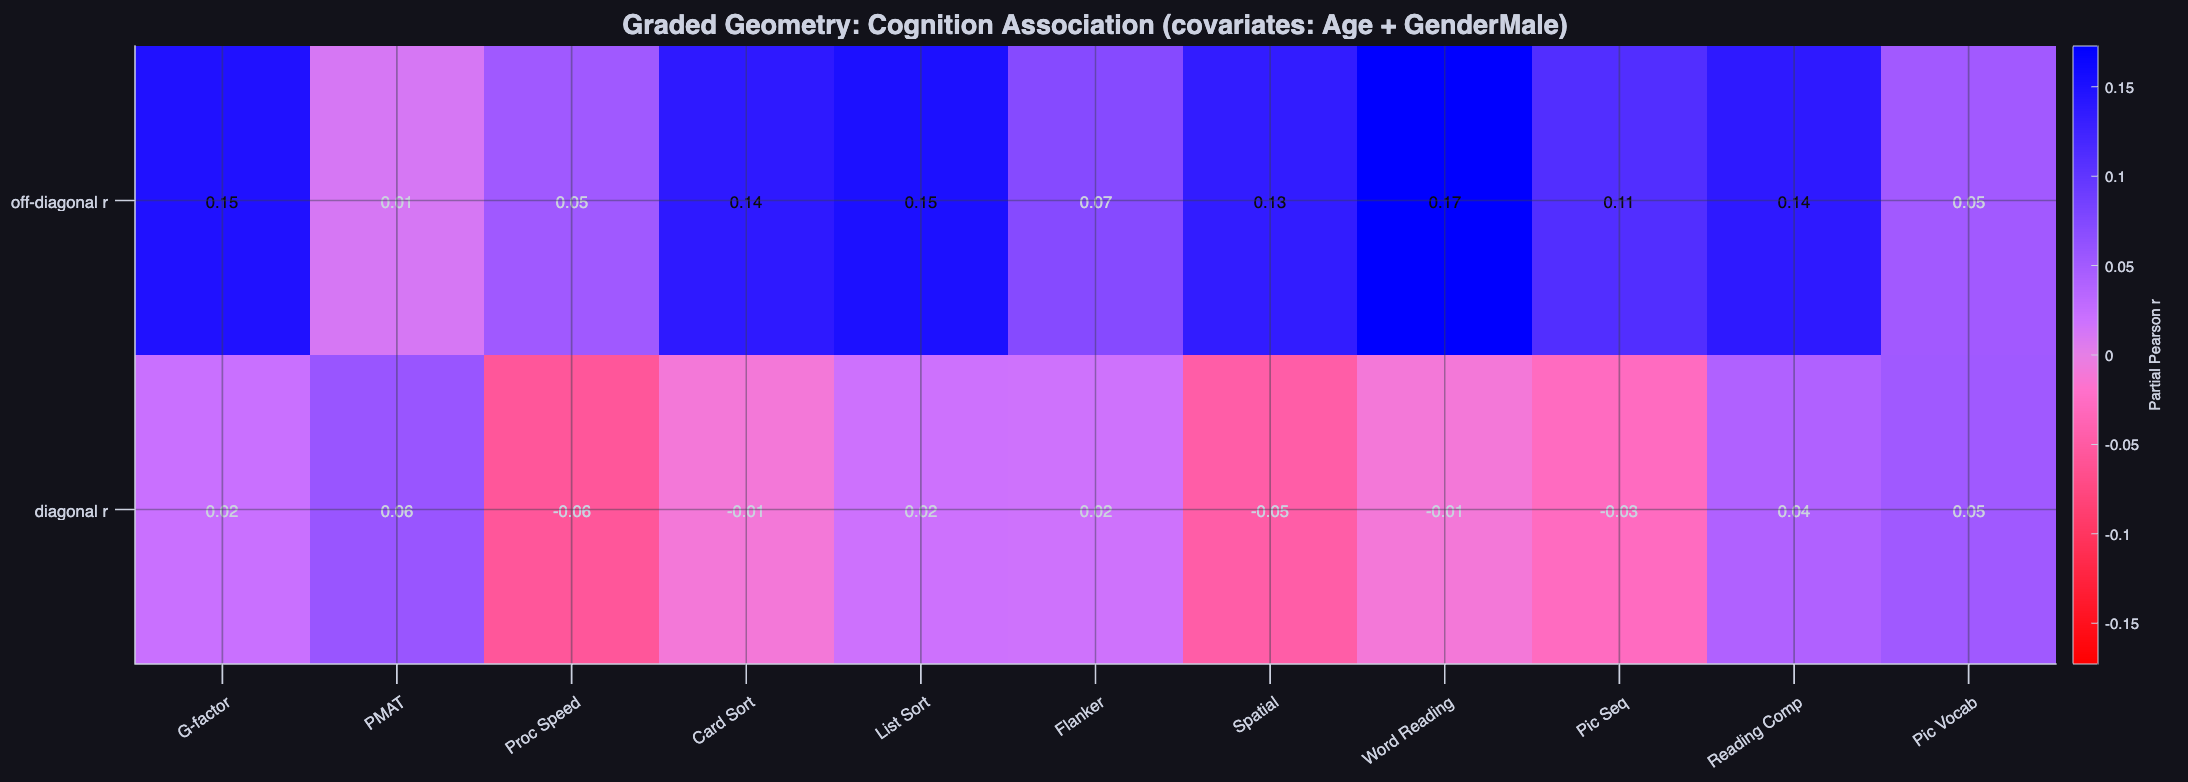
\includegraphics[width=\textwidth]{figures/appendix/a09_geometry_cognition.png}};
\begin{scope}[x={(image.south east)},y={(image.north west)}]
\node[panel label] at (0.01,0.98) {A};
\end{scope}
\end{tikzpicture}
\caption{\textbf{Associations between graded-geometry fit and cognition.}
\textbf{(A)} Heatmap of age- and sex-adjusted partial Pearson correlations between participant-level held-out geometry fit and cognitive measures. Effects were weak and none survived false-discovery-rate correction.}
\label{fig:app-geometry-cognition}
\end{figure}

\begin{figure}[p]
\centering
\begin{tikzpicture}
\node[anchor=south west,inner sep=0] (image) at (0,0)
  {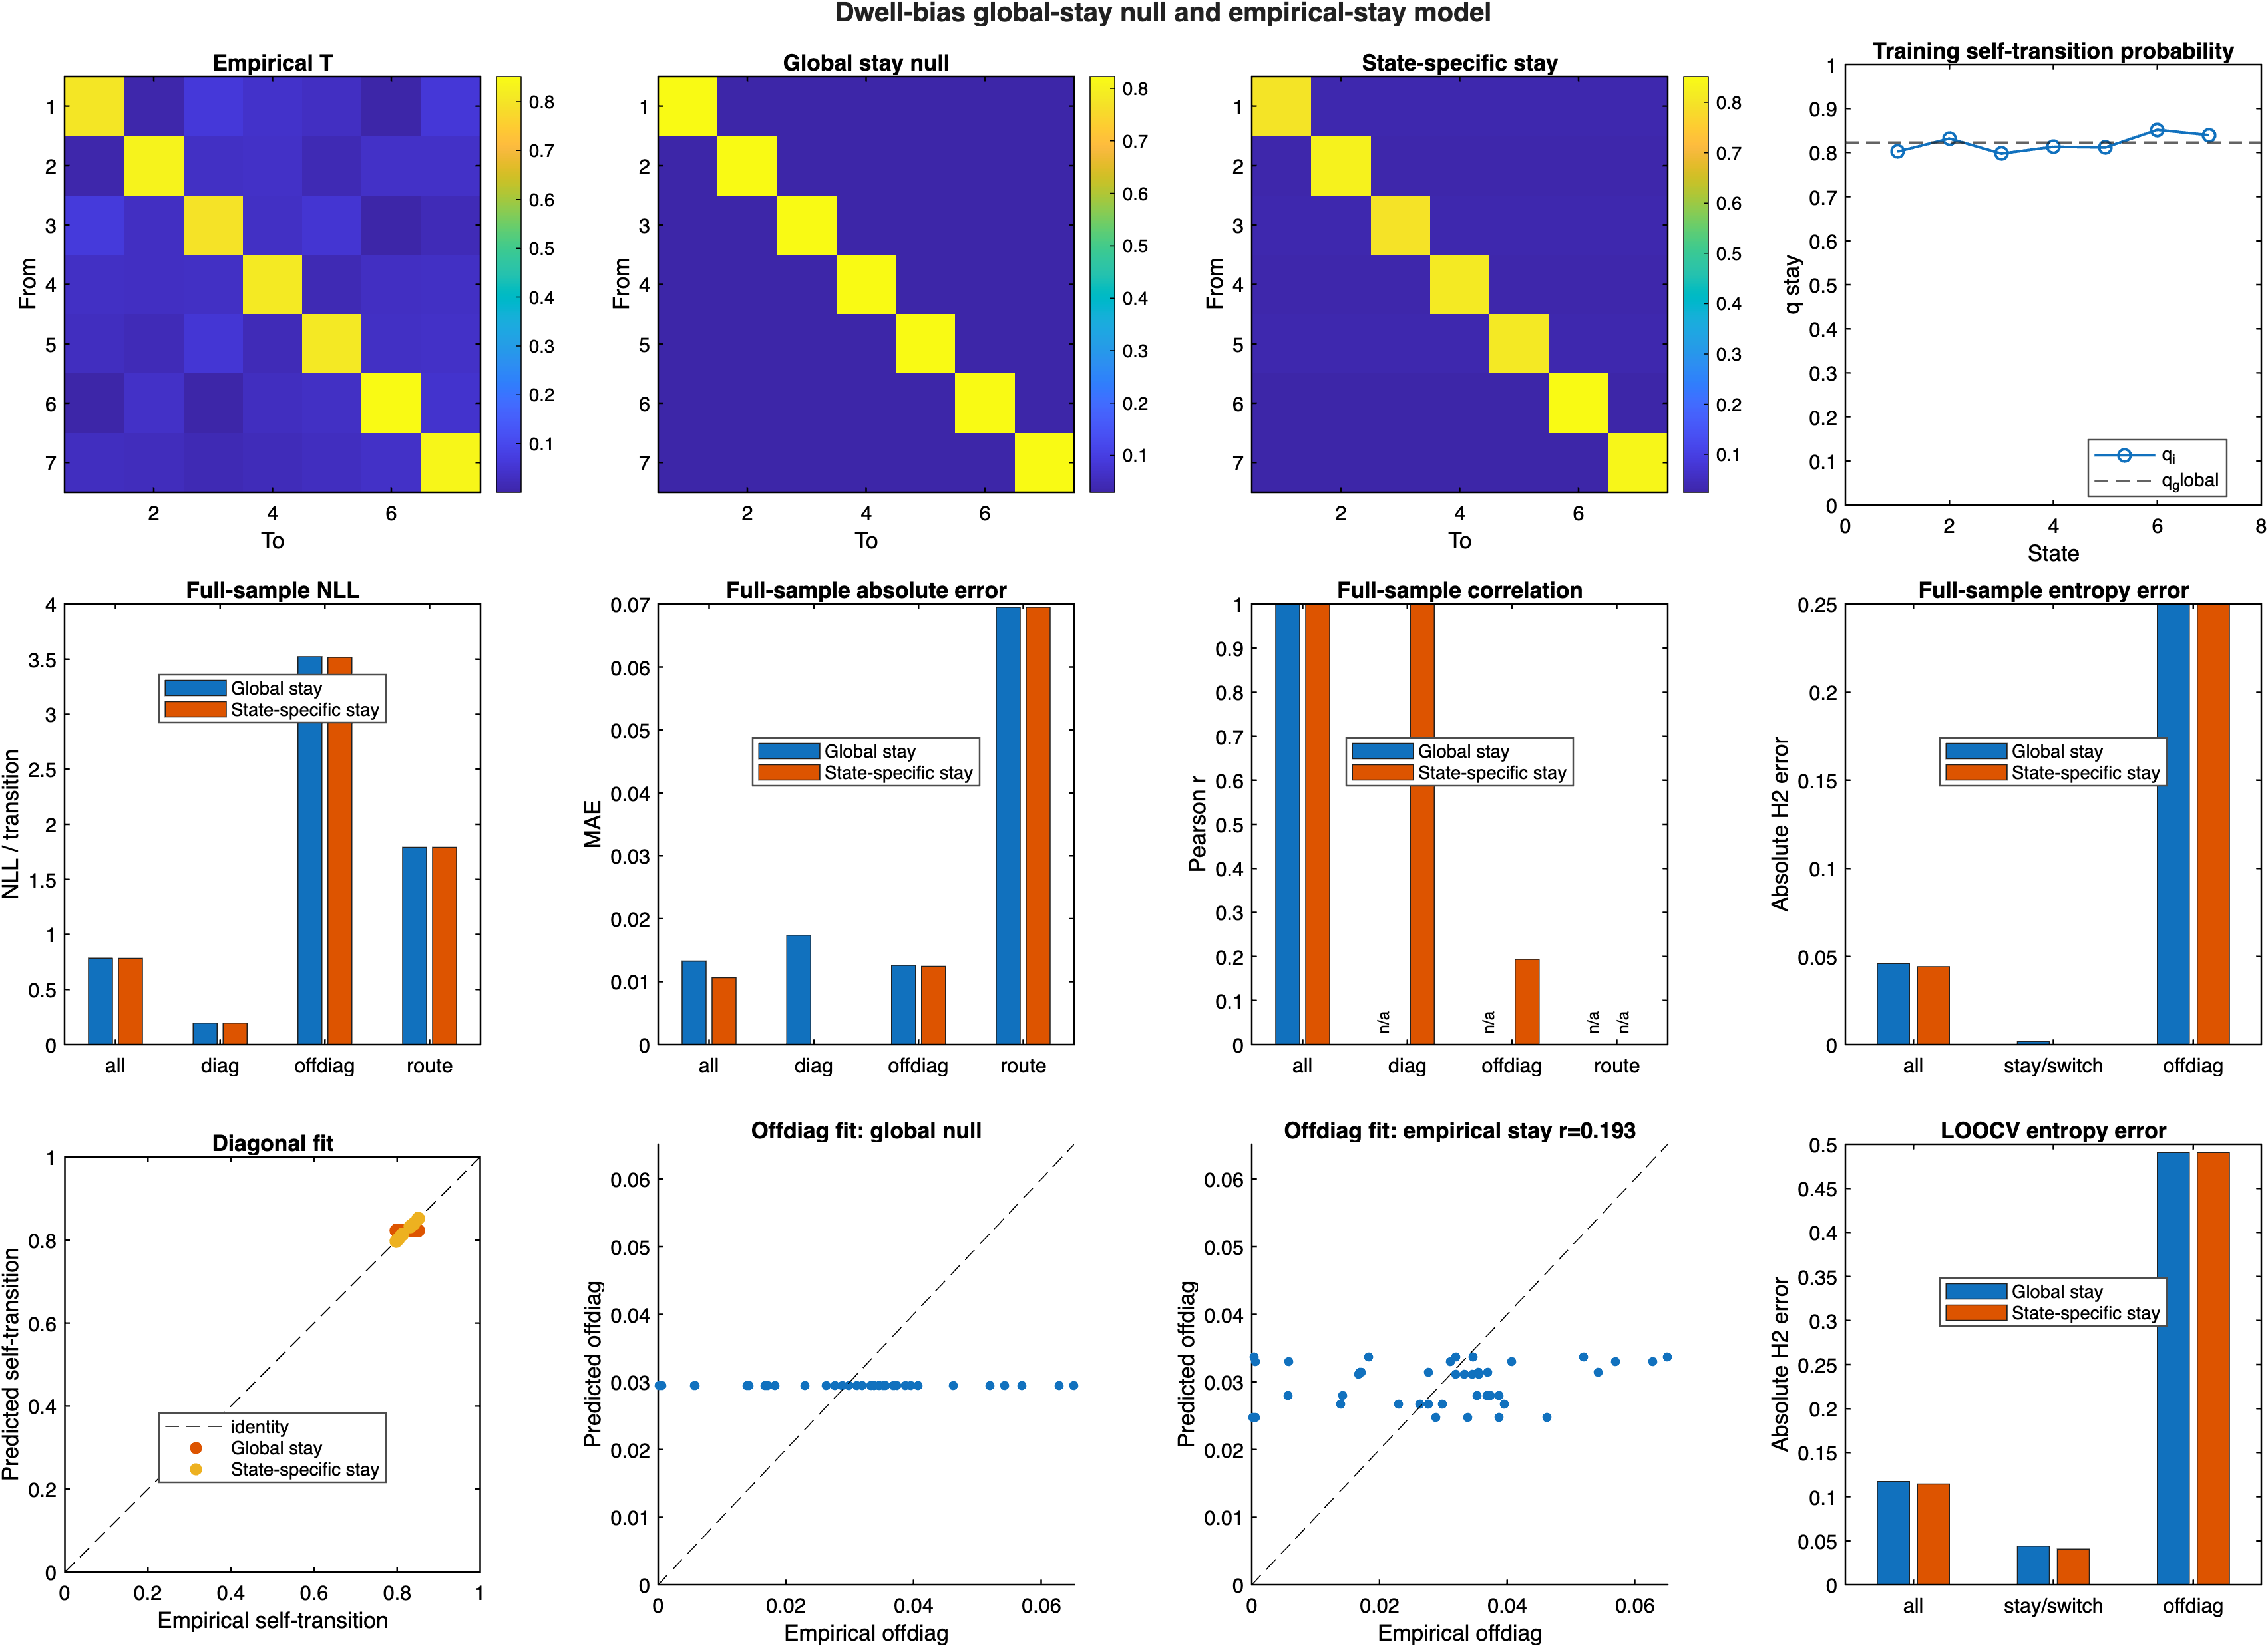
\includegraphics[width=\textwidth]{figures/appendix/a10_dwell_bias.png}};
\begin{scope}[x={(image.south east)},y={(image.north west)}]
\node[panel label] at (0.01,0.98) {A};
\node[panel label] at (0.26,0.98) {B};
\node[panel label] at (0.51,0.98) {C};
\node[panel label] at (0.76,0.98) {D};
\node[panel label] at (0.01,0.65) {E};
\node[panel label] at (0.26,0.65) {F};
\node[panel label] at (0.51,0.65) {G};
\node[panel label] at (0.76,0.65) {H};
\node[panel label] at (0.01,0.32) {I};
\node[panel label] at (0.26,0.32) {J};
\node[panel label] at (0.51,0.32) {K};
\node[panel label] at (0.76,0.32) {L};
\end{scope}
\end{tikzpicture}
\caption{\textbf{Global-stay and state-specific stay models.}
\textbf{(A)} Empirical transition matrix.
\textbf{(B)} Global-stay null.
\textbf{(C)} State-specific stay model.
\textbf{(D)} Training self-transition probabilities.
\textbf{(E)} Full-sample NLL.
\textbf{(F)} Absolute probability error.
\textbf{(G)} Predicted--empirical correlation.
\textbf{(H)} Entropy error.
\textbf{(I)} Diagonal fit.
\textbf{(J)} Off-diagonal fit under the global null.
\textbf{(K)} Off-diagonal fit with empirical stay rates.
\textbf{(L)} Held-out entropy error.}
\label{fig:app-dwell-bias}
\end{figure}

\begin{figure}[p]
\centering
\begin{tikzpicture}
\node[anchor=south west,inner sep=0] (image) at (0,0)
  {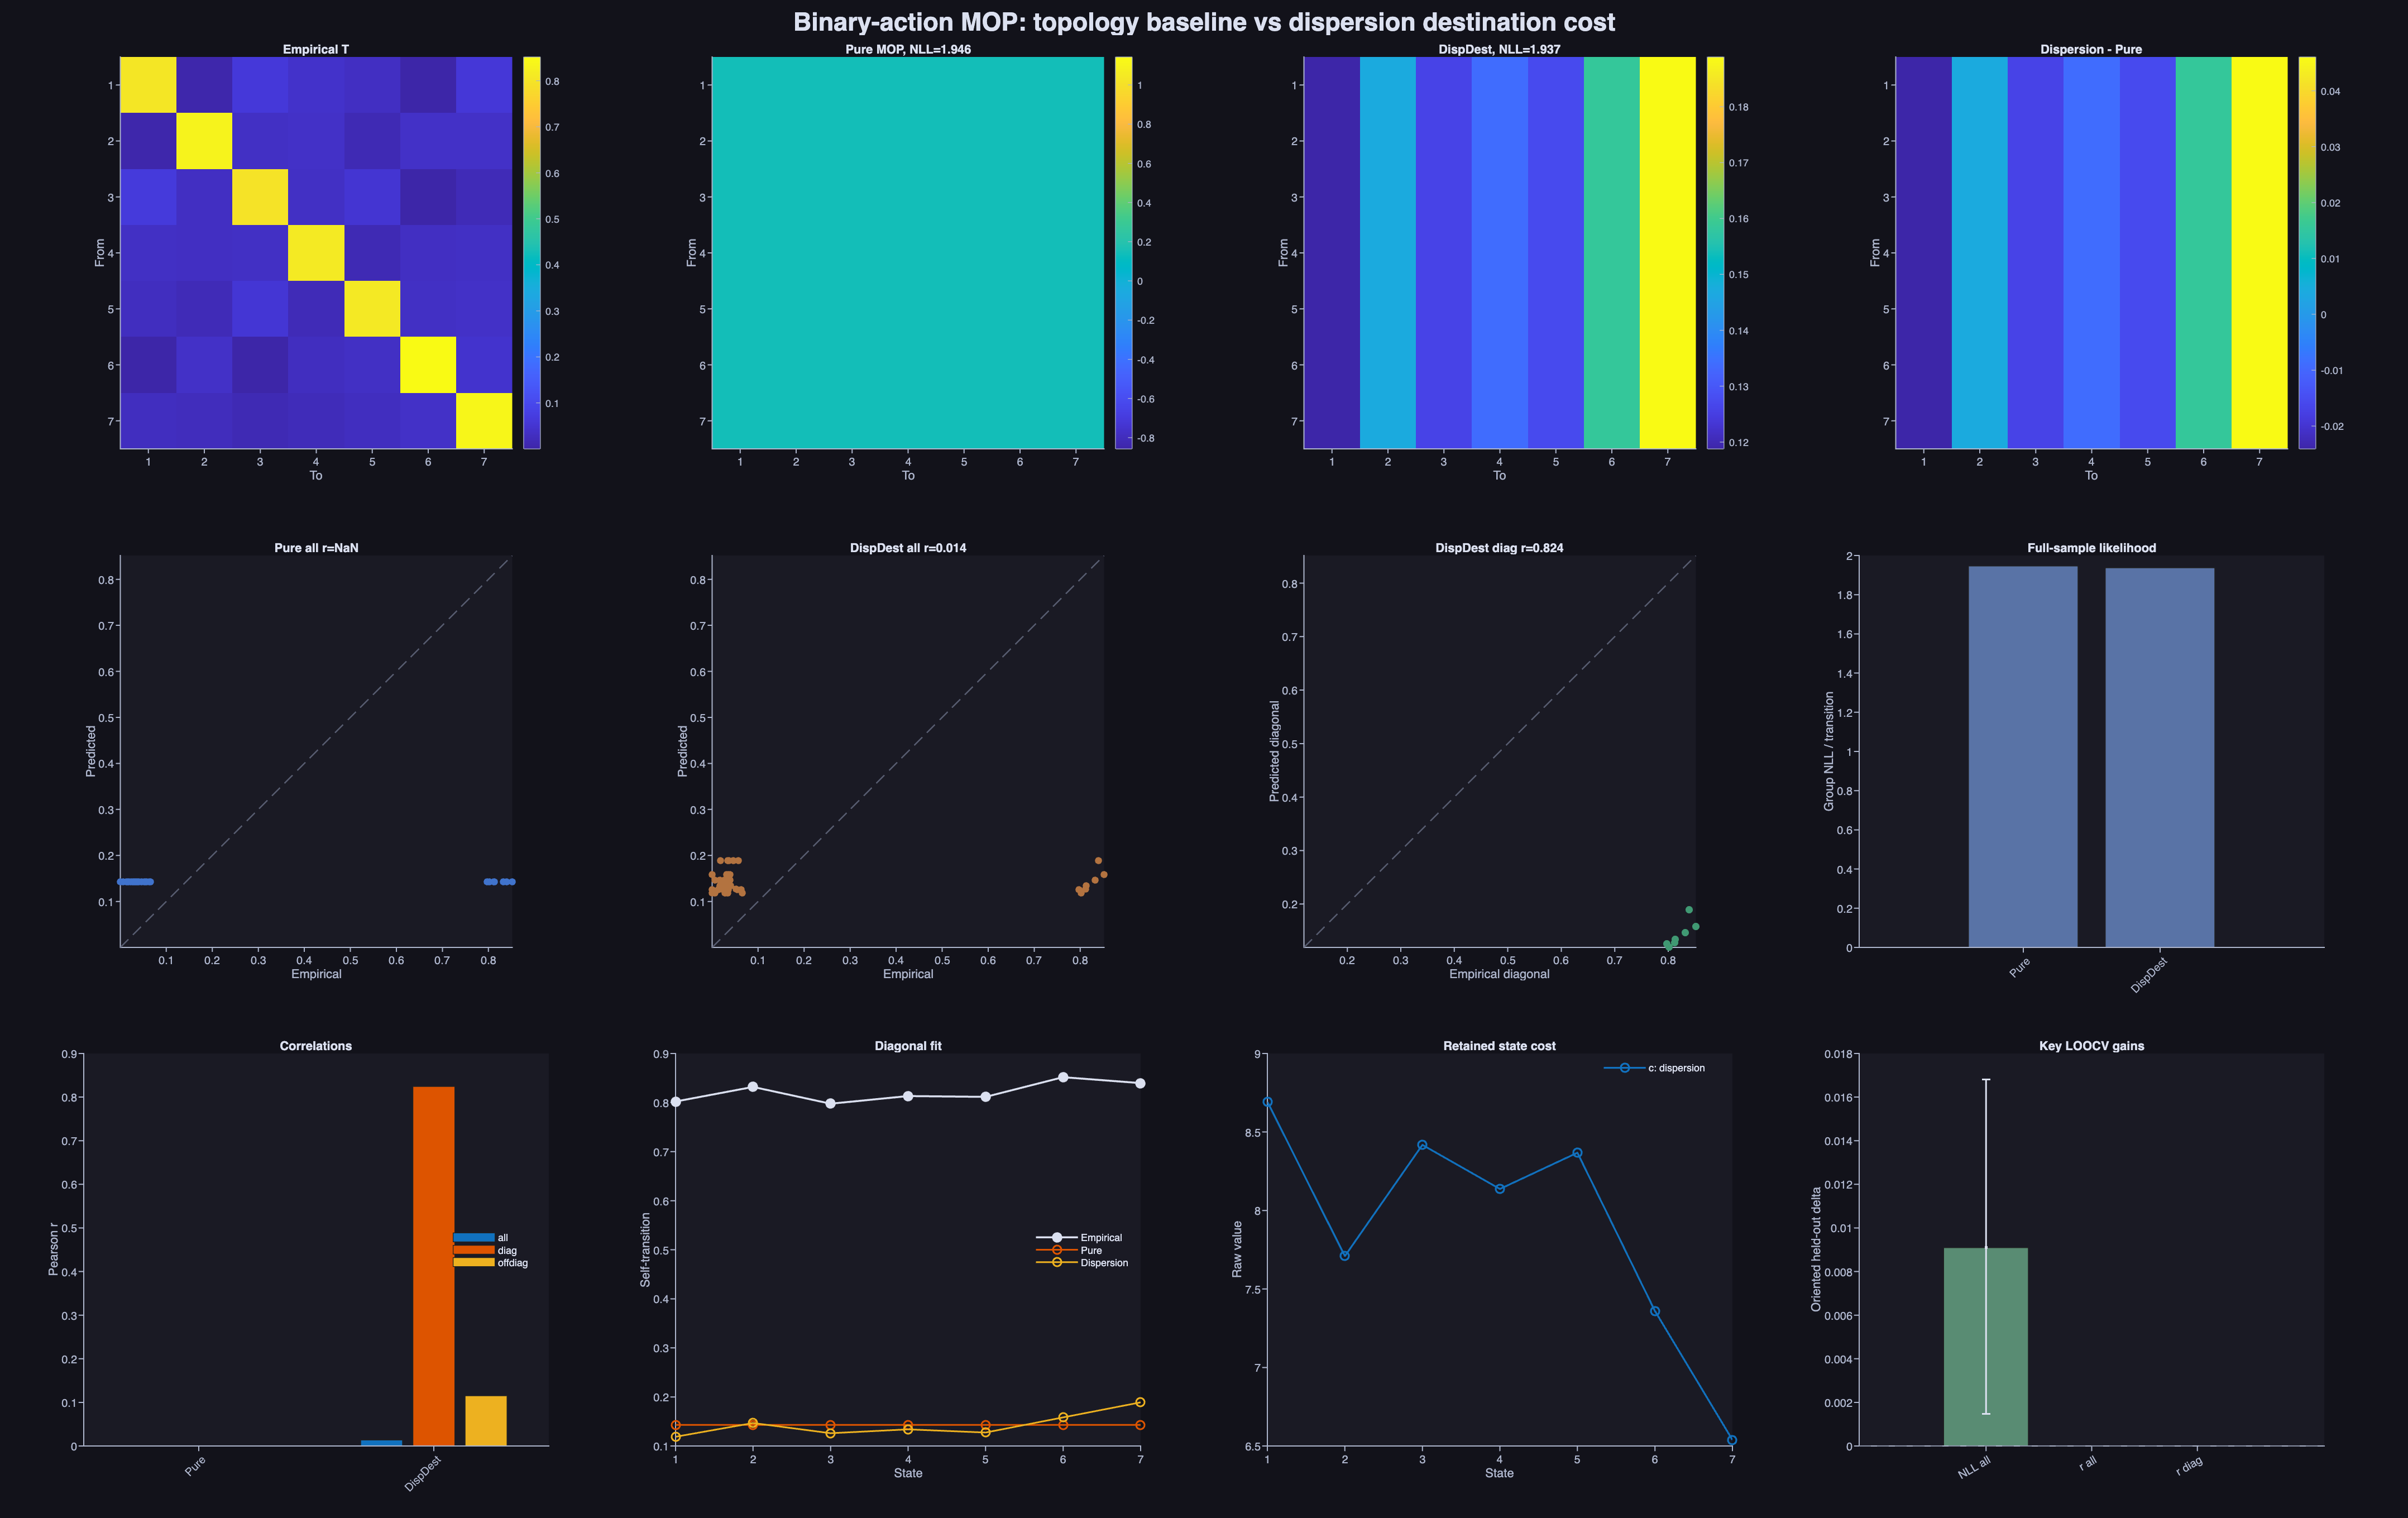
\includegraphics[width=\textwidth]{figures/appendix/a11_binary_mop.png}};
\begin{scope}[x={(image.south east)},y={(image.north west)}]
\node[panel label] at (0.01,0.98) {A};
\node[panel label] at (0.26,0.98) {B};
\node[panel label] at (0.51,0.98) {C};
\node[panel label] at (0.76,0.98) {D};
\node[panel label] at (0.01,0.65) {E};
\node[panel label] at (0.26,0.65) {F};
\node[panel label] at (0.51,0.65) {G};
\node[panel label] at (0.76,0.65) {H};
\node[panel label] at (0.01,0.32) {I};
\node[panel label] at (0.26,0.32) {J};
\node[panel label] at (0.51,0.32) {K};
\node[panel label] at (0.76,0.32) {L};
\end{scope}
\end{tikzpicture}
\caption{\textbf{Binary-action maximum-occupancy comparison.}
\textbf{(A)} Empirical transition matrix.
\textbf{(B)} Pure MOP prediction.
\textbf{(C)} Dispersion-cost prediction.
\textbf{(D)} Difference between fitted matrices.
\textbf{(E)} Pure-MOP predicted versus empirical probabilities.
\textbf{(F)} Dispersion-model fit for all entries.
\textbf{(G)} Dispersion-model diagonal fit.
\textbf{(H)} Full-sample likelihood.
\textbf{(I)} Predicted--empirical correlations.
\textbf{(J)} Diagonal performance.
\textbf{(K)} Retained destination-cost estimate.
\textbf{(L)} Key held-out improvements.}
\label{fig:app-binary-mop}
\end{figure}

\begin{figure}[p]
\centering
\begin{tikzpicture}
\node[anchor=south west,inner sep=0] (image) at (0,0)
  {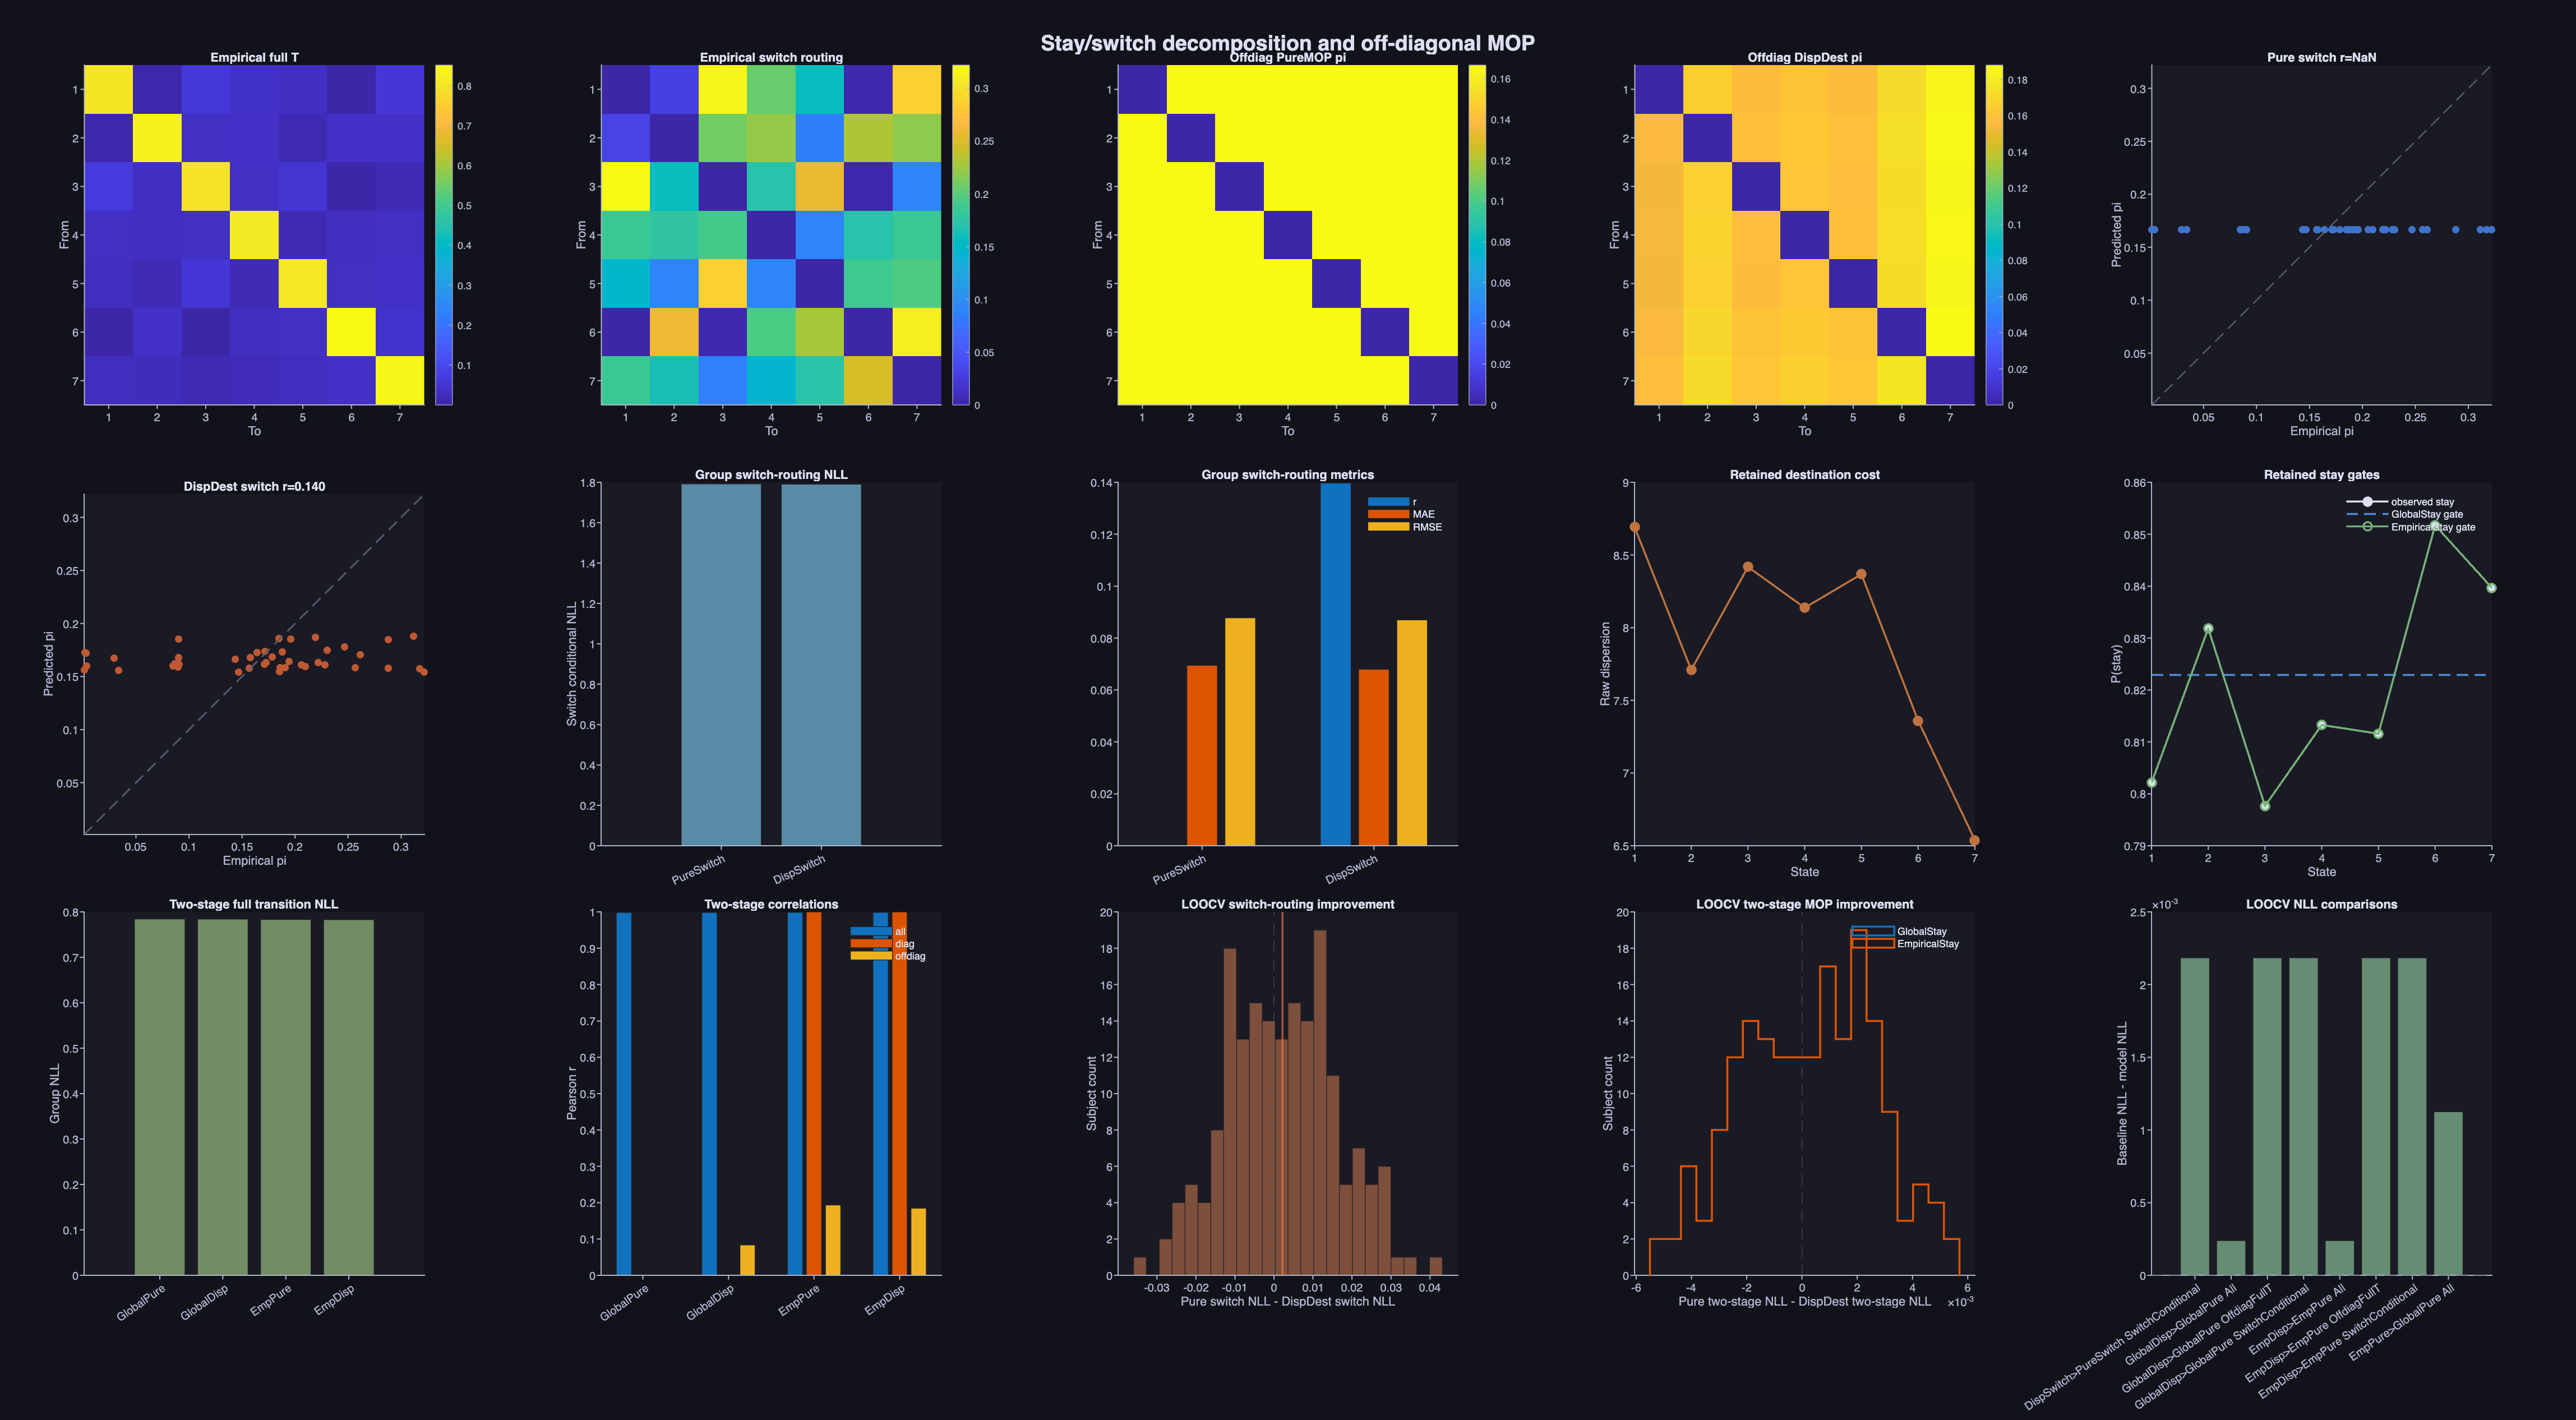
\includegraphics[width=\textwidth]{figures/appendix/a12_stay_switch_mop.png}};
\begin{scope}[x={(image.south east)},y={(image.north west)}]
\node[panel label] at (0.01,0.98) {A};
\node[panel label] at (0.21,0.98) {B};
\node[panel label] at (0.41,0.98) {C};
\node[panel label] at (0.61,0.98) {D};
\node[panel label] at (0.81,0.98) {E};
\node[panel label] at (0.01,0.65) {F};
\node[panel label] at (0.21,0.65) {G};
\node[panel label] at (0.41,0.65) {H};
\node[panel label] at (0.61,0.65) {I};
\node[panel label] at (0.81,0.65) {J};
\node[panel label] at (0.01,0.32) {K};
\node[panel label] at (0.21,0.32) {L};
\node[panel label] at (0.41,0.32) {M};
\node[panel label] at (0.61,0.32) {N};
\node[panel label] at (0.81,0.32) {O};
\end{scope}
\end{tikzpicture}
\caption{\textbf{Stay/switch decomposition and off-diagonal MOP comparison.}
\textbf{(A)} Empirical full transition matrix.
\textbf{(B)} Empirical switch-routing matrix.
\textbf{(C)} Topology-only switch policy.
\textbf{(D)} Dispersion-cost switch policy.
\textbf{(E--F)} Predicted versus empirical routing for the two policies.
\textbf{(G)} Group switch-routing NLL.
\textbf{(H)} Group routing metrics.
\textbf{(I)} Retained destination cost.
\textbf{(J)} Retained stay gates.
\textbf{(K)} Two-stage full-transition NLL.
\textbf{(L)} Two-stage correlations.
\textbf{(M)} Held-out switch-routing improvement.
\textbf{(N)} Held-out two-stage MOP improvement.
\textbf{(O)} Held-out NLL comparison.}
\label{fig:app-stay-switch-mop}
\end{figure}

\clearpage
\section{Entropy and cognition}

\begin{figure}[htbp]
\centering
\begin{tikzpicture}
\node[anchor=south west,inner sep=0] (image) at (0,0)
  {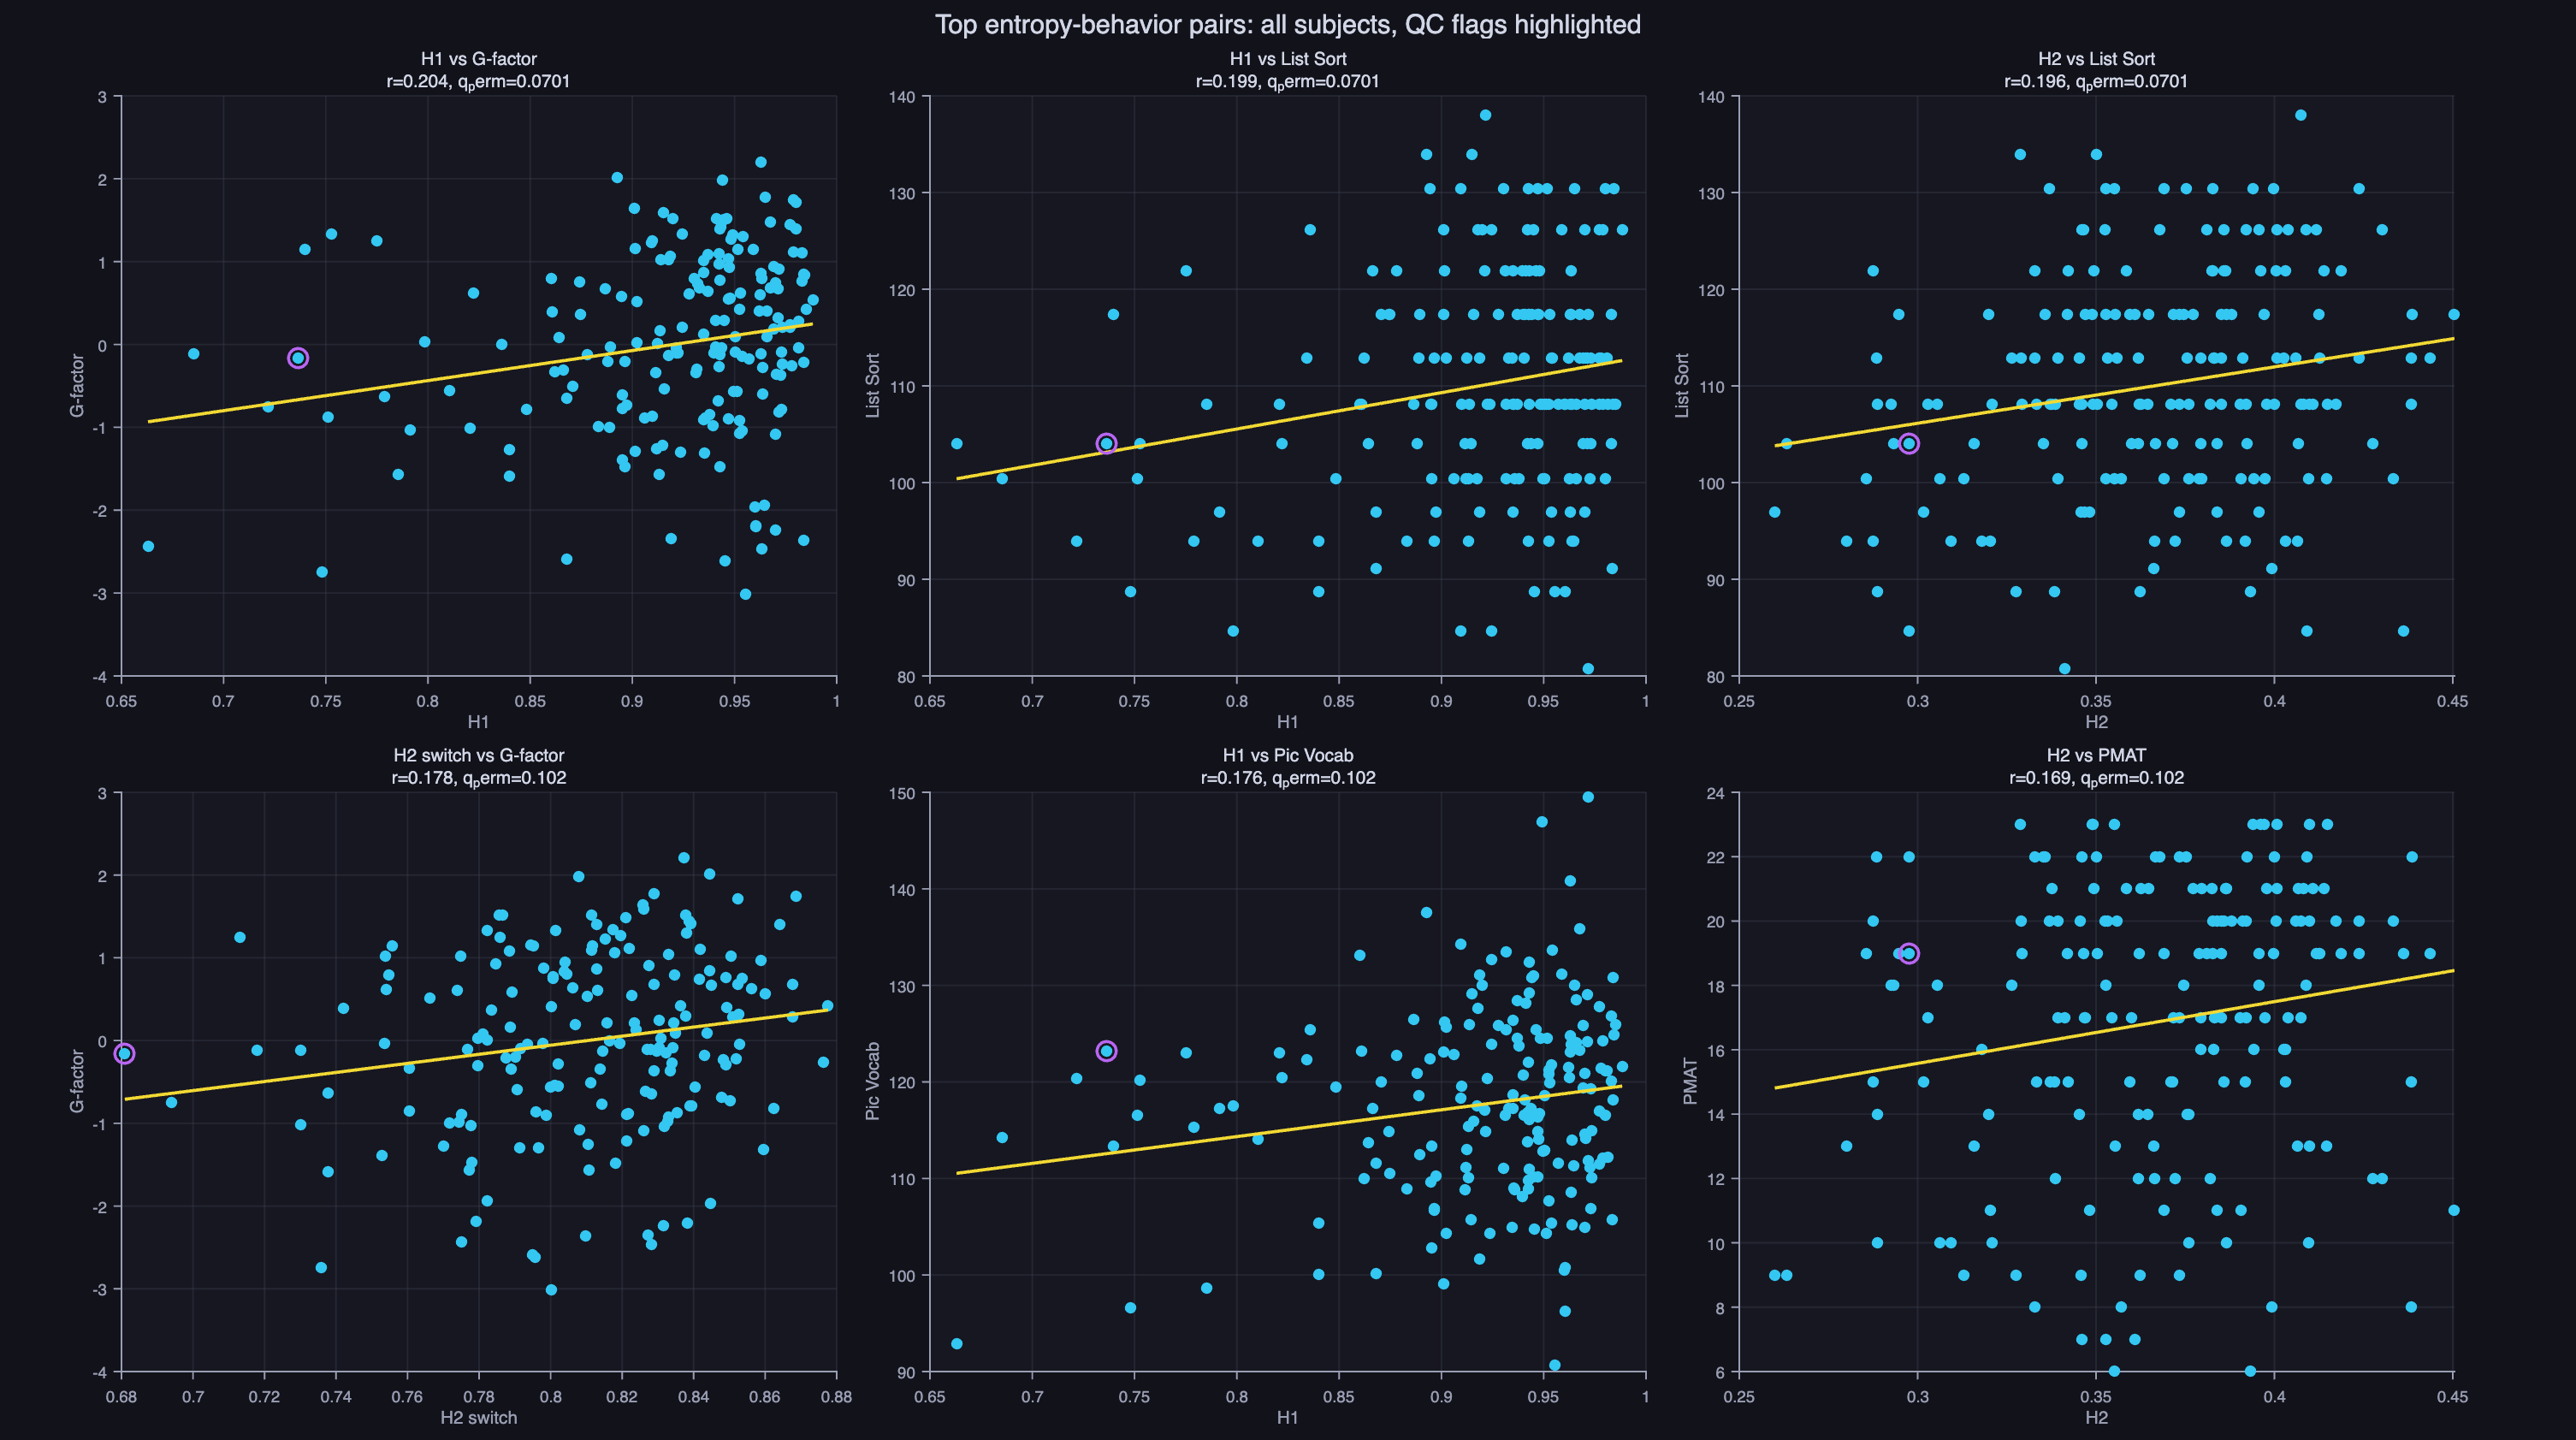
\includegraphics[width=\textwidth]{figures/appendix/a13_entropy_scatterplots.png}};
\begin{scope}[x={(image.south east)},y={(image.north west)}]
\node[panel label] at (0.01,0.98) {A};
\node[panel label] at (0.34,0.98) {B};
\node[panel label] at (0.67,0.98) {C};
\node[panel label] at (0.01,0.49) {D};
\node[panel label] at (0.34,0.49) {E};
\node[panel label] at (0.67,0.49) {F};
\end{scope}
\end{tikzpicture}
\caption{\textbf{Leading normalized entropy--cognition associations.}
\textbf{(A)} $H_1$ versus general cognitive factor.
\textbf{(B)} $H_1$ versus List Sorting.
\textbf{(C)} $H_2$ versus List Sorting.
\textbf{(D)} $H_{2,\mathrm{switch}}$ versus general cognitive factor.
\textbf{(E)} $H_1$ versus Picture Vocabulary.
\textbf{(F)} $H_2$ versus Penn Matrix Reasoning.
Lines are ordinary least-squares fits; the highlighted point is the prespecified sensitivity case.}
\label{fig:app-entropy-scatters}
\end{figure}

\begin{figure}[p]
\centering
\begin{tikzpicture}
\node[anchor=south west,inner sep=0] (image) at (0,0)
  {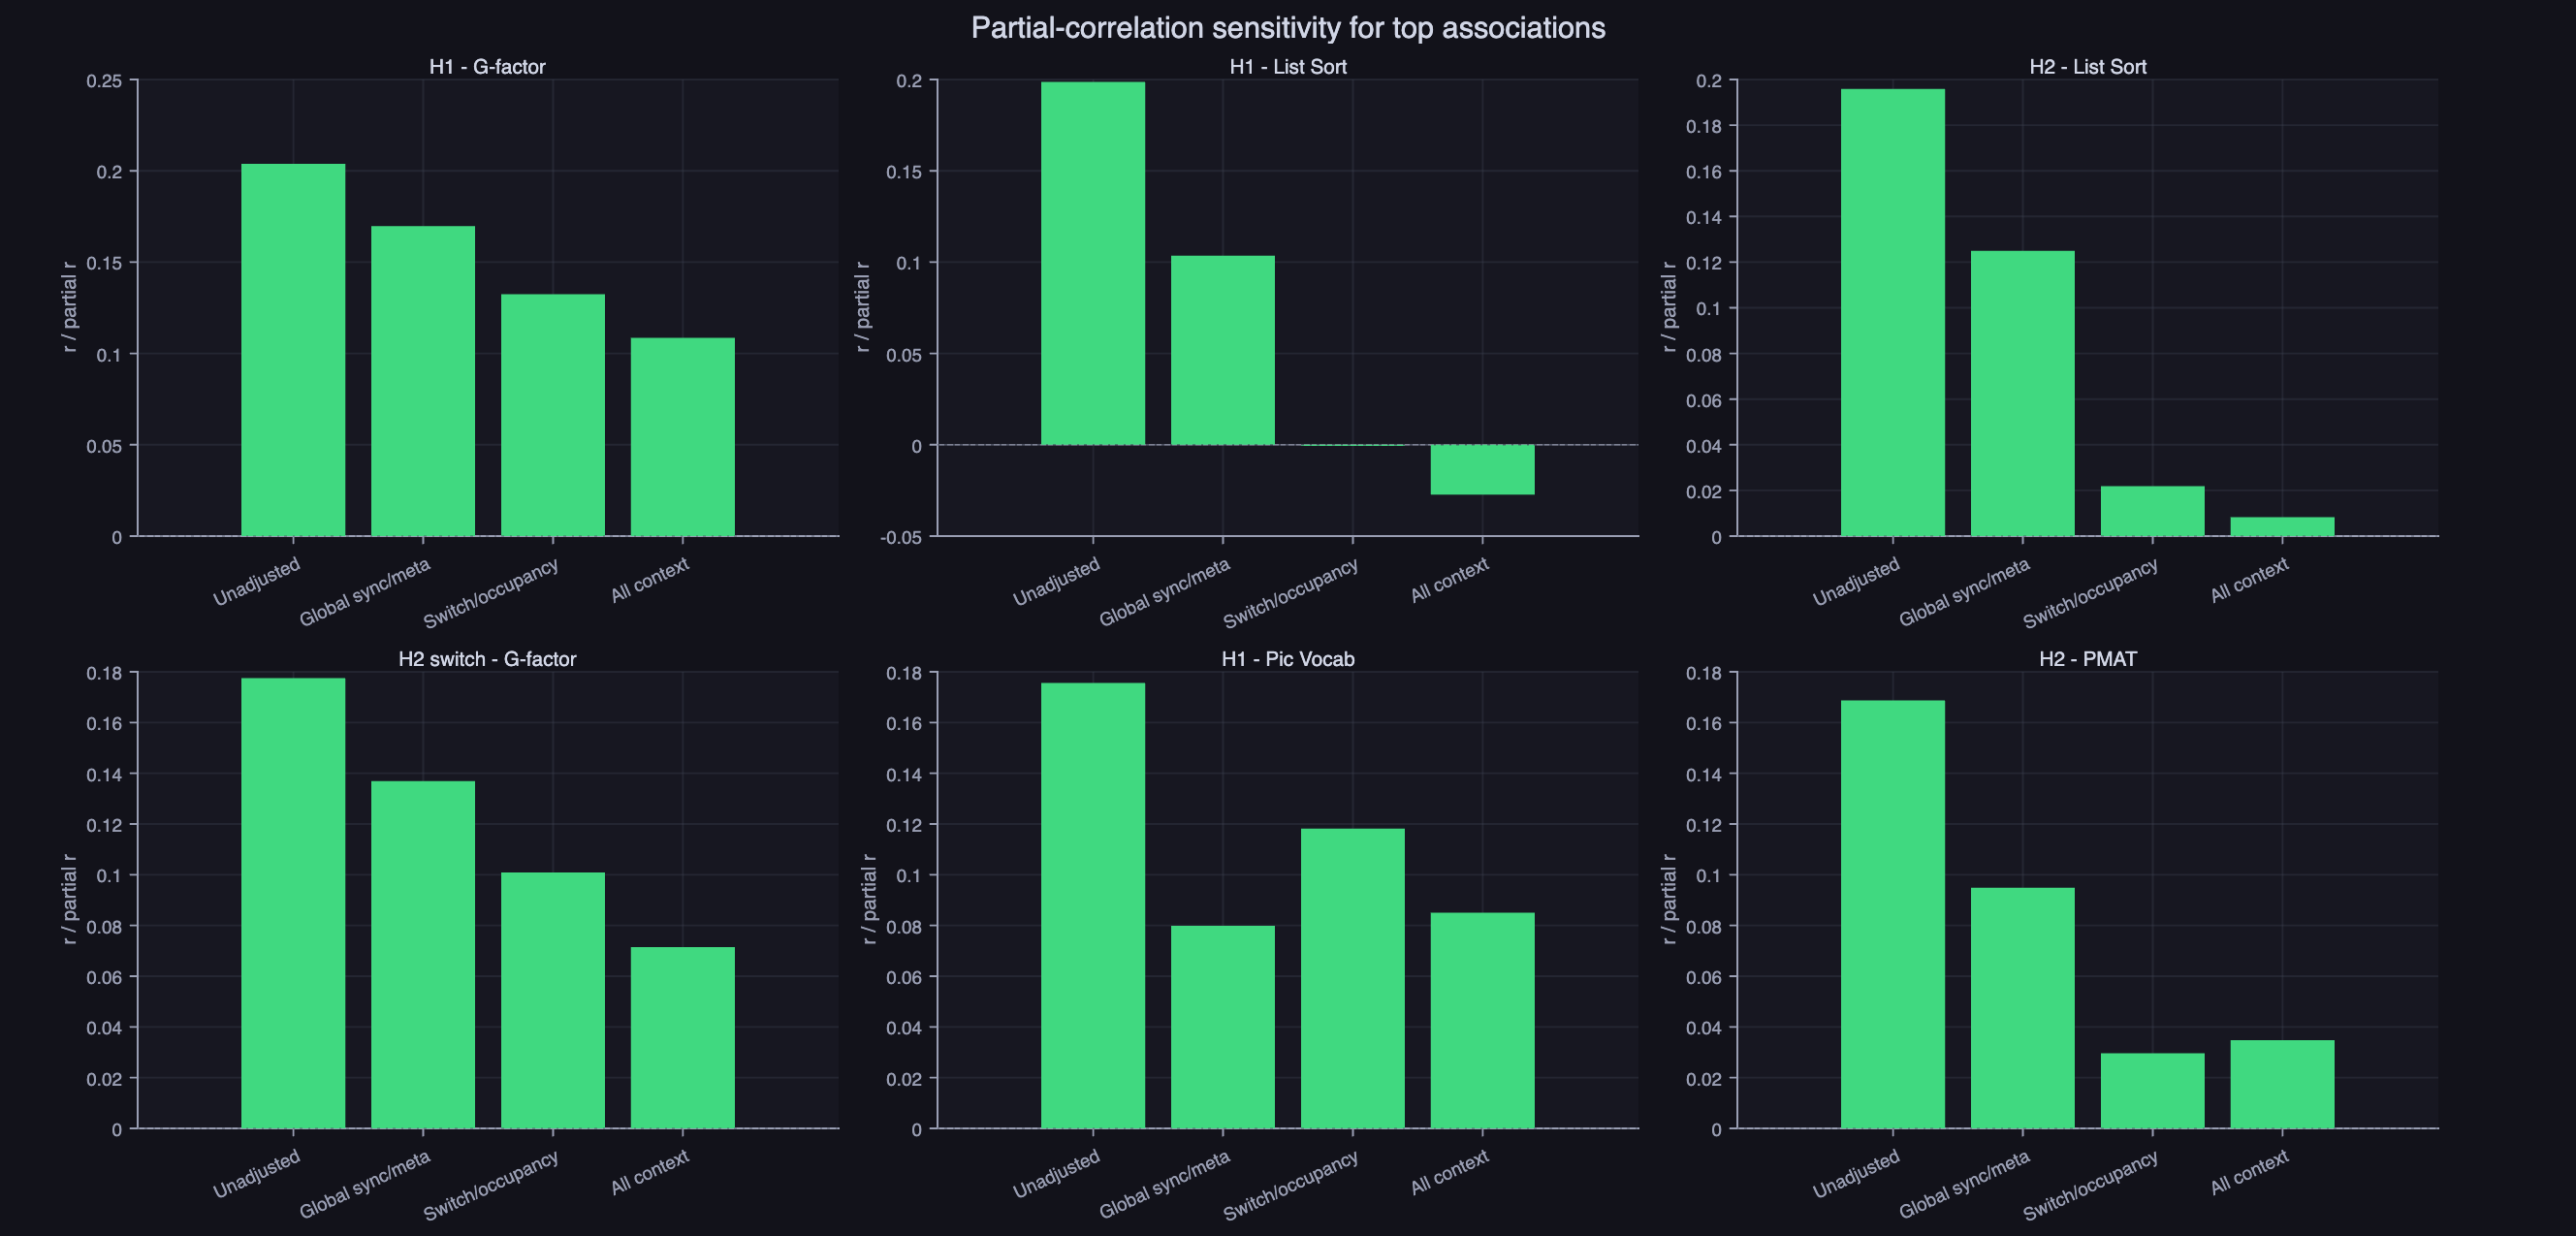
\includegraphics[width=\textwidth]{figures/appendix/a14_entropy_partial_sensitivity.png}};
\begin{scope}[x={(image.south east)},y={(image.north west)}]
\node[panel label] at (0.01,0.98) {A};
\node[panel label] at (0.34,0.98) {B};
\node[panel label] at (0.67,0.98) {C};
\node[panel label] at (0.01,0.49) {D};
\node[panel label] at (0.34,0.49) {E};
\node[panel label] at (0.67,0.49) {F};
\end{scope}
\end{tikzpicture}
\caption{\textbf{Contextual sensitivity of entropy--cognition associations.}
\textbf{(A)} $H_1$--general-factor association.
\textbf{(B)} $H_1$--List-Sorting association.
\textbf{(C)} $H_2$--List-Sorting association.
\textbf{(D)} $H_{2,\mathrm{switch}}$--general-factor association.
\textbf{(E)} $H_1$--Picture-Vocabulary association.
\textbf{(F)} $H_2$--Penn-Matrix association.
Each panel compares the unadjusted correlation with correlations adjusted for synchronization context, switching and occupancy, or all contextual measures.}
\label{fig:app-entropy-partial}
\end{figure}

\begin{figure}[p]
\centering
\begin{tikzpicture}
\node[anchor=south west,inner sep=0] (image) at (0,0)
  {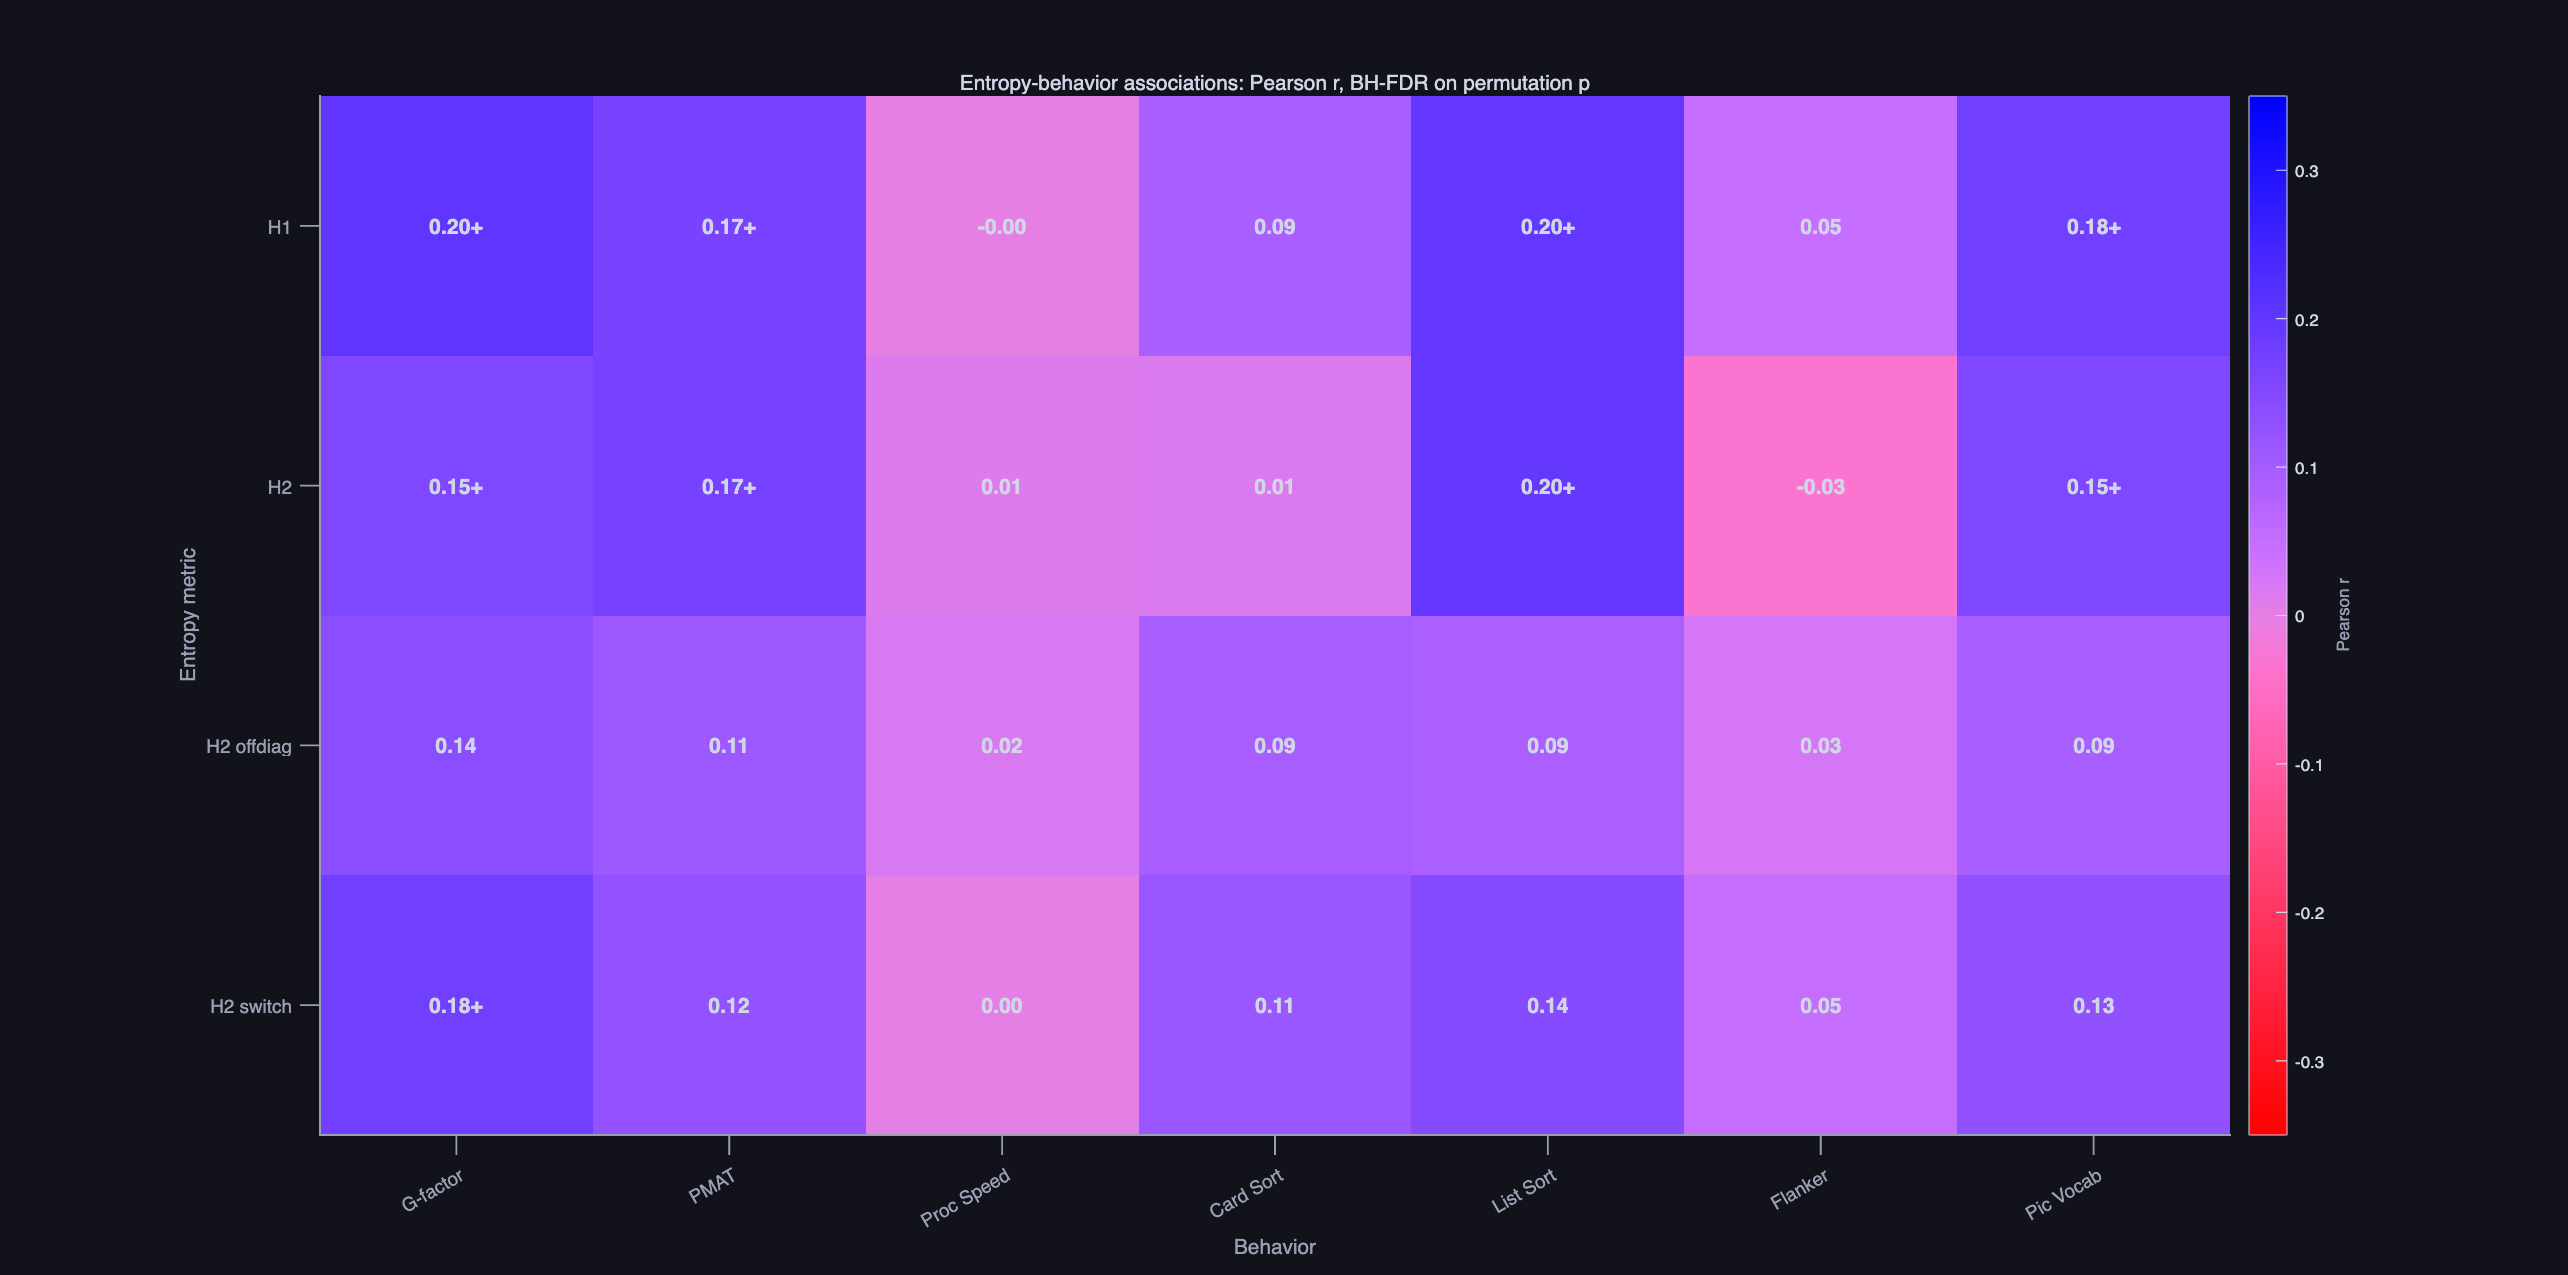
\includegraphics[width=\textwidth]{figures/appendix/a15_entropy_cognition_heatmap.png}};
\begin{scope}[x={(image.south east)},y={(image.north west)}]
\node[panel label] at (0.01,0.98) {A};
\end{scope}
\end{tikzpicture}
\caption{\textbf{Normalized entropy--cognition association matrix.}
\textbf{(A)} Pearson correlations between four normalized entropy measures and seven cognitive outcomes. A plus sign denotes an uncorrected permutation result below 0.05; no cell survived false-discovery-rate correction across the full family.}
\label{fig:app-entropy-cognition}
\end{figure}

\clearpage
\end{document}
